\documentclass[]{report}

\usepackage[utf8]{inputenc}

\usepackage{eurosym}
\usepackage[
  margin=1.8cm,
  includefoot,
  footskip=10pt,
]{geometry}
\usepackage{graphicx}
\graphicspath{{figures/}}
\usepackage[french]{babel}
\usepackage{url}
\usepackage[colorlinks=true, linkcolor=black, urlcolor=blue]{hyperref}
\usepackage{color}
\usepackage[dvipsnames]{xcolor}
\usepackage{titling}
\usepackage{subfig}
\usepackage[bottom]{footmisc}
\usepackage{amsmath}
\usepackage{enumitem}

\usepackage{algorithm}
\usepackage{algpseudocode}
\floatname{algorithm}{Procédure}
\renewcommand{\algorithmicreturn}{\textbf{retourne}}
\renewcommand{\algorithmicprocedure}{\textbf{procédure}}
\renewcommand{\algorithmicrequire}{\textbf{Entrée:}}
\renewcommand{\algorithmicensure}{\textbf{Sortie:}}
%\renewcommand{\algorithmiccomment}[1]{\{#1\}}
\renewcommand{\algorithmicend}{\textbf{fin}}
\renewcommand{\algorithmicif}{\textbf{si}}
\renewcommand{\algorithmicthen}{\textbf{alors}}
\renewcommand{\algorithmicelse}{\textbf{sinon}}
\renewcommand{\algorithmicfor}{\textbf{pour}}
\renewcommand{\algorithmicforall}{\textbf{pour tout}}
\renewcommand{\algorithmicdo}{\textbf{faire}}
\renewcommand{\algorithmicwhile}{\textbf{tant que}}
\newcommand{\algorithmicelsif}{\algorithmicelse\ \algorithmicif}
\newcommand{\algorithmicendif}{\algorithmicend\ \algorithmicif}
\newcommand{\algorithmicendfor}{\algorithmicend\ \algorithmicfor}

\newcommand{\minit}[1]{\noindent{\small\textbf{ \underline{#1}}}~\\}
\newcommand{\todo}[1]{\par{\color{red} /---| A faire : #1 |---\textbackslash\\}}
\newcommand{\todoIL}[1]{{\color{red}[todo: #1]}}
\newcommand{\wordlink}[2]{\hyperref[#2]{#1~\ref{#2}}}
\newcommand{\floor}[1]{\left\lfloor #1 \right\rfloor}

\setcounter{secnumdepth}{3}

%-- Logos PDG --
\pretitle{
\vspace{-5cm}
\vfill
~\\
~\\
~\\
~\\
\begin{center}
\begin{figure}[!ht]
	\centering
	\begin{minipage}{0.5\textwidth}
		\centering
		\LARGE
		\hspace{1.5cm}
		\textbf{Université de Mons}
		\normalsize
	\end{minipage}\hfill
	\begin{minipage}{0.5\textwidth}
		\centering
		
\includegraphics[width=0.4\textwidth]{UMons_logo}
	\end{minipage}	
\end{figure}

\begin{center}
\begin{figure}[!ht]
	\centering
	\begin{minipage}{0.5\textwidth}
		\centering
		\LARGE
		\hspace{1.5cm}
		\textbf{Faculté des Sciences}
		\normalsize
	\end{minipage}\hfill
	\begin{minipage}{0.5\textwidth}
		\centering
		
\includegraphics[width=0.35\textwidth]{sciences_logo}
	\end{minipage}	
\end{figure}
\end{center}
\vfill
%
%\begin{figure}[!tbp]
%  \centering
%  \subfloat{
\includegraphics[width=0.25\textwidth]{UMons_logo.png}}
%  \hfill
%  \subfloat{
\includegraphics[width=0.25\textwidth]{sciences_logo.png}}\\
%\end{figure}
%~\newline

}

\posttitle{\end{center}}

\begin{document}

\title{
\vspace{2cm}
\noindent\fbox{\parbox{\textwidth}
{
\centering
~\\
{\huge Performance des mécanismes de sécurité\\ \vspace{0.2cm} du framework 6TiSCH}\\
~\\
}}
}



\author{
\LARGE{Mémoire de fin d'études}\\
\LARGE{par}\\
~\vspace{0.4cm}
\LARGE{Rémy DECOCQ}\\
~\\
~\\
\Large
Directeur : M$^{\text{r}}$ Bruno QUOITIN\\
Service des Réseaux et Télécommunications
\normalsize
}

\date{
\vspace{10cm}
\Large
Année Académique 2019-2020}

\maketitle          

\thispagestyle{empty}   

\newpage
~
\newpage

\begin{center}
\textbf{\LARGE Remerciements}\\
\end{center}
~\\
~\\
~\\
\Large
\par Au terme de la rédaction de ce travail de fin d'études, je souhaite exprimer toute ma gratitude au personnel encadrant et à mes proches qui m'ont soutenu, contribuant de près ou de loin à ce mémoire.\\

Ma plus profonde reconnaissance à mon professeur et encadrant principal M$^{\text{r}}$ Bruno Quoitin, dont le suivi actif et les relectures attentives ont permis de mener ce travail a bien. Mes remerciements à David Hauweele dont l'implication volontaire a permis de concrétiser l'obtention de résultats.\\

Enfin, mes remerciements aux rapporteurs et au jury pour l'attention portée à l'évaluation de ce travail.
\normalsize

\newpage
~
\newpage

\vspace{5cm}
~\\

\begin{center}
\textbf{\Large Performance des mécanismes de sécurité du framework 6TiSCH}\\
~\\
{\Large Rémy DECOCQ}\\
~\\
\textbf{\Large RÉSUMÉ}
\end{center}
\vspace{2cm}

\large
Les réseaux de capteurs sans-fils sont au cœur des applications industrielles de l'Internet des Objets (\textit{Industrial IoT}). Ces réseaux présentent la particularité d'être composés de noeuds restreints en ressources et d'être déployés dans des environnements où les communic	tions radios sont rendues difficiles. Dans de telles conditions, l'utilisation d'une pile réseau classique telle que \textit{TCP/IP} n'est pas envisageable. Depuis 2013, le groupe de travail 6TiSCH à l'IETF travaille à la standardisation d'une pile adaptée à de tels réseaux. Cette pile 6TiSCH, bien que différente de la pile TCP/IP, permet des communications IP et donc une interconnectivité du réseau de capteur avec Internet.\\

Ce travail établit la structure typique d'un réseau dans lequel peut être déployée la pile. Une analyse de la pile 6TiSCH dans sa globalité est menée, dépeignant chaque couche qui la compose et les concepts qui y sont définis, ainsi que l'interaction entre ces couches. Ayant introduit ces différentes couches essentielles à sa compréhension, une attention particulière est portée au mécanisme qui permet à un nouveau noeud de rejoindre un réseau 6TiSCH actif. Cette \textit{joining phase} est analysée en détails du point de vue de la sécurité. Effectivement, la joining phase est un procédé critique en terme de performances et sécurité.  Après avoir introduit les solutions proposées par les standards, un nouveau schéma désigné par ``méthode NPEB" est proposé pour améliorer les performances de la joining phase. Une série d'expérimentations en simulateur sont alors menées pour d'une part évaluer la joining phase standard avec et sans mécanisme de sécurité et d'autre part mesurer les gains de performances la méthode NPEB proposée.\\

\vspace{2cm}

\textbf{Mot-clés :} WSN, Industrial IoT, TSCH, pile 6TiSCH, joining phase 

\normalsize

\newpage
~
\newpage

\tableofcontents

\newpage

\newgeometry{margin=2.3cm,
  includefoot,
  footskip=8pt,}

\section*{Introduction}


Les réseaux de capteurs sont devenus monnaie courante dans l'industrie, on estime en 2020 que plusieurs dizaines de milliers de réseaux ont été déployés, comptabilisant plus de 18 milliards d'heures de fonctionnement. Originellement, ces réseaux fonctionnaient sur des standards propriétaires tels que WirelessHART et ISA100.1a \cite{stack-IoT}. Bien que capables de performances acceptables en pratique grâce à l'emplois du principe TSCH (\textit{Time Slotted Channel Hopping}) \cite{decentralized}, ces piles réseaux n'offrent pas un connectivité IP et ne s'inscrivent donc pas dans la tendance générale de l'IoT, dont l'interconnectivité avec Internet est une ligne directrice \cite{stack-IoT}. Le groupe de travail 6TiSCH est créé à l'IETF en 2013 avec pour double objectif de standardiser l'adoption de TSCH dans les réseaux de capteurs 802.15.4 et d'élaborer un pile réseau supportant les communications IP pour ces réseaux restreints. L'ensemble de spécifications produites constitue ce que l'on appelle la pile 6TiSCH.\\

Ce travail caractérise ces réseaux sans-fil restreints, leur architecture typique et les contraintes qui justifient l'élaboration d'une pile réseau adaptée. L'intégralité des différentes couches qui composent la pile 6TiSCH sont passées en revue, ainsi que la façon dont elles interagissent entre elles pour constituer une pile déployable et efficace dans un réseau sans-fil restreint. Une attention particulière est portée à la \textit{joining phase 6TiSCH}, qui dénote la façon dont un nouveau noeud rejoint un réseau 6TiSCH déjà actif. Plus particulièrement, la sécurisation de cette procédure, qui est une phase critique, est analysée en détail. Des expérimentations sont menées en simulateur pour illustrer l'impact de la sécurité sur la joining phase, et une méthode est proposée pour améliorer les performances de la joining phase.\\

Ce document est divisée en deux parties principales. La première partie constitue un état de l'art de la pile 6TiSCH dans sa globalité et des caractéristiques des réseaux dans lesquels elle est destinée à être déployée. Le \wordlink{Chapitre}{chap_intro} introduit les réseaux sans-fil restreints, l'évolution des standards et groupes de travail y contribuant et la technologie TSCH qui est le fondement de la pile 6TiSCH. Le \wordlink{Chapitre}{chap_6TiSCH} précise l'architecture typique des réseaux considérés et établit une analyse couche par couche de la pile 6TiSCH et des principes qui lui sont propres. Finalement, le \wordlink{Chapitre}{joining_analysis} se concentre sur la joining phase qui fait intervenir les différentes couches présentées précédemment, en mettant l'accent sur les mécanismes de sécurité qui la protègent. La seconde partie fait l'état d'un travail expérimental sur la joining phase. Le \wordlink{Chapitre}{chap_NPEB} présente la méthode NPEB, qui est une proposition de nouveau schéma pour l'amélioration des performances de la joining phase. Le \wordlink{Chapter}{chap_exp} concentre les expérimentations effectuées sur la joining phase en simulateur : des métriques pertinentes sont sélectionnées pour d'une part illustrer l'impact de la sécurité sur celle-ci et d'autre part démontrer les gains de performance apportés par la méthode NPEB.



\chapter{Présentation du standard IEEE802.15.4 et TSCH}
\label{chap_intro}
\newpage

\section{L'IoT, les réseaux sans fils et leurs contraintes}
\label{WSNs}

L'Internet de Objets (\textit{Internet of Things }- IoT) couvre de nombreux domaines d'applications tels que les \textit{smart}-\textit{homes}/\textit{buildings}/\textit{cities}, les soins de santé et les transports entre autres. Les équipements que l'on regroupe généralement derrière cette dénomination sont de nature variée : capteurs et actionneurs, périphériques de communication/multimédias, domotique, etc. mais s'accordent sur un point : ils sont connectés et tendent à l'être avec le réseau Internet. Également, comme ce sont généralement des équipements embarqués, ils sont restreints en ressources telles que l'énergie (alimentation par batterie), la puissance d'émission radio, la capacité mémoire et les performances CPU. Ces limitations ont conduit à la conception et la standardisation de nombreux protocoles qui y sont adaptés afin de rendre possible et efficace la communication en réseau de ces objets.\\

\par Cela est particulièrement vrai pour l'IIoT (\textit{Industrial IoT}) qui regroupe des secteurs tels que l'industrie agricole, l'automatisation des usines, la gestion des stocks, etc. Effectivement, l'optimisation apportée par ces protocoles adaptés est un facteur clé pour augmenter la rentabilité du déploiement de tels réseaux. Ils permettent également de déployer de façon plus efficace des réseaux de capteurs sans fils, dits WSNs (\textit{Wireless Sensors Networks}), qui sont a priori peu adaptés aux contraintes des systèmes embarqués, notamment au niveau de la consommation énergétique imputée aux transmissions radios qui sont coûteuses. Les protocoles de communication qui orchestrent les WSNs sont donc conçus dans une optique de compromis entre la minimisation de la consommation énergétique des nœuds qui les composent et la fiabilité désirée de ces communications (délais, bande passante et déterminisme). La pile réseau 6TiSCH étudiée dans ce document est un ensemble de protocoles et principes qui apportent une réponse concrète à ces besoins.\\

\par Les WSNs étant des systèmes de communication restreints, ils font partie de ce qu'on appelle les LLNs (\textit{Low-power and Lossy Networks}). L'implémentation d'une pile réseau pour les LLNs doit tenir compte de leurs caractéristiques qui sont principalement les suivantes :\\

\begin{itemize}
\item[$\bullet$] Présence du phénomène de \textit{multipath fading} lié à la réflexion d'ondes surtout en environnement clos et métallique (usine) illustré par la \wordlink{Figure}{fig:multipath} et interférences extérieures/d'autres nœuds proches
\vspace{0.2cm}
\item[$\bullet$] Forte densité de nœuds entraînant des interférences et possiblement déployés de façon imprécise à des endroits non déterminés
\vspace{0.2cm}
\item[$\bullet$] Nœuds limités en ressources énergétiques, pour lesquels il est donc très coûteux de laisser leur radio allumée
\vspace{0.2cm}
\item[$\bullet$] Radios peu puissantes, taux de transmission et portée faibles entraînant parfois le besoin de transmissions \textit{multi-hop}
\vspace{0.2cm}
\item[$\bullet$] Nœuds limités en ressources CPU, mémoire et stockage
\vspace{0.2cm}
\item[$\bullet$] Changements réguliers dans la topologie, mobilité des nœuds et décalages entre leur horloges respectives
\end{itemize}
~\\


À titre d'exemple, un nœud TelosB (illustré par la \wordlink{Figure}{fig:telosb}) typiquement utilisable dans un WSN mais considéré comme peu performant, présente les caractéristiques suivantes : microcontrôleur 16-bit et processeur cadencé à 8 MHz, disposant de 10 kB de RAM et 48 kB de mémoire flash. Il est couplable avec une radio CC2420 supportant le standard 802.15.4, opérant dans la bande de fréquence 2.4-2.485 GHz. Cette radio draine 25.8 mA en transmettant et 18.8 mA en recevant. Si la source d'alimentation du nœud est comparable à celle d'une paire de piles AA (3000 mAh de charge), et que la radio reste allumée en écoutant le canal sans arrêt alors le nœud vivra $\frac{3000\: mAh}{18.8\: mA} \approx 159\: h$. Cette hypothèse revient à considérer un \textit{duty cycle} (portion de temps pendant laquelle la radio est allumée) de 100\%. Selon \cite{stack-IoT}, une pile de communication efficace devrait aboutir à un duty cycle bien en dessous de 1\%. On porterait alors la durée de vie du nœud à $\frac{3000\:mAh}{18.8\: mAh \times 1\%} \approx 160000\:h \approx 22 $ mois.\\

\newpage

\begin{figure}[!ht]
	\centering
	\begin{minipage}{0.43\textwidth}
		\centering
		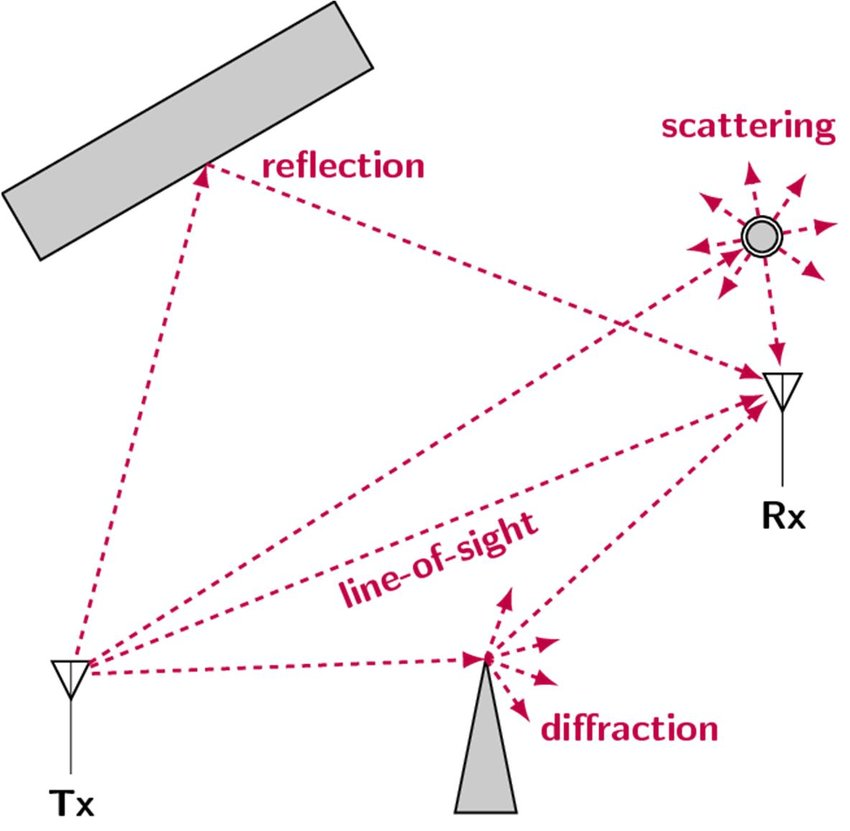
\includegraphics[width=\textwidth]{multipath}
		\caption{Phénomène de multipath fading\cite{multipath}}
		\label{fig:multipath}
	\end{minipage}\hfill
	\begin{minipage}{0.43\textwidth}
		\centering
		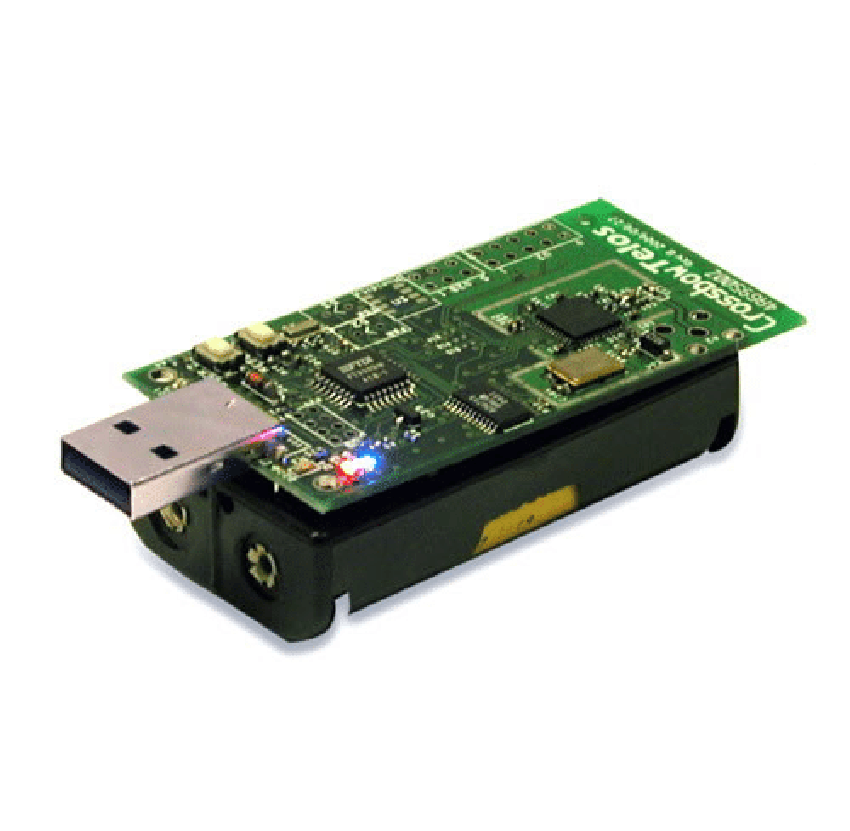
\includegraphics[width=\textwidth]{TelosB}
		\caption{Microcontrôleur TelosB, Texas Instruments \cite{telosb}}
		\label{fig:telosb}
	\end{minipage}	
\end{figure}


\par La technologie TSCH (détaillée dans la \wordlink{section}{tschfond}) apporte une réponse efficace aux problématiques des WSNs induites par leurs caractéristiques évoquées plus haut. Les optimisations apportées par TSCH aux WSNs permettent d'envisager des grandeurs de durée de vie du réseau de l'ordre de la décennie \cite{SODA}, se traduisant donc par des gains conséquents pour les industries. Ainsi, de nombreux standards et piles réseaux (propriétaires ou non) ont été développés en se basant sur la pierre d'angle TSCH. 6TiSCH en fait partie intégrante. De façon plus généralisée, un pile réseau qui est destinée à faire communiquer des équipements restreints dans la vision actuelle de l'(I)IoT devrait présenter les qualités suivantes \cite{stack-IoT} :\\
\begin{itemize}
\vspace{0.2cm}
\item[$\bullet$] Une consommation minimale de l'énergie et des communications limitées au strict nécessaire
\vspace{0.2cm}
\item[$\bullet$] Une fiabilité maximale des transmissions par rapport aux besoins et à la qualité de service attendue
\vspace{0.2cm}
\item[$\bullet$] Une transparence des communications vers les réseaux extérieurs, sous-entendu l'Internet \cite{6TiSCH-industrial-perf}
\end{itemize}

\newpage

\section{L'évolution des standards - amendement 802.15.4e et 6TiSCH}

En 2013, l'IEEE Standards Association sort un standard de communication définissant des couches physique et lien (PHY et MAC) adaptées aux communications radios dans les LLNs. Le standard IEEE802.15.4 devient alors le standard \textit{de facto} utilisé dans ces environnements restreints \cite{6top-perf}, prodiguant une base solide par dessus laquelle de nombreuses piles réseaux complètes (majoritairement propriétaires) se développent. Ainsi, en 2004 la ZigBee Alliance distribue la pile Zigbee 1.0, qui est l'implémentation d'une spécification propriétaire calquant les plus bas niveaux de sa pile sur le standard IEEE802.15.4 PHY/MAC. Elle se base sur une topologie en étoile capable de \textit{multi-hop}, utilisant les notions de coordination entre PANs (Personal Area Network) et de différenciation des types de nœuds en fonction de leur (in)capacité à servir de coordinateur entre PANs ou entre nœuds \cite{stack-IoT}.\\

\par Cependant, cette conception liée au standard 802.15.4 souffre de certaines limitations parmi lesquelles :\\

\begin{itemize}
\item[$\bullet$] le canal de transmission ne varie pas dans le temps, exposant les communications à des interférences sans pouvoir y réagir si elles restent constantes dans ce canal
\vspace{0.2cm}
\item[$\bullet$] la synchronisation temporelle partielle : il est possible à un nœud de réserver un moment dans le temps où il pourra émettre sans risque de collision, mais dans tous les cas il devra faire usage de CSMA/CA, ce qui est coûteux en terme d'énergie
\vspace{0.2cm}
\item[$\bullet$] les nœuds faisant office de coordinateur sont actifs tout du long de la période d'activité prévue pour qu'un nœud normal entame une communication
\vspace{0.2cm}
\item[$\bullet$] les communications avec un réseau IP (donc Internet) ne sont pas gérées
\end{itemize}
~\\
\par Pour passer au dessus de certaines de ces limitations, un nouveau standard baptisé TSMP (\textit{Time Synchronized Mesh Protocol}) est commercialisé en 2004 par la société Dust Networks. Ce dernier apporte une révolution dans la conception des paradigmes de communication propres aux LLNs : la combinaison des principes de TDMA (\textit{Time Division Multiple Access}) et FDMA (\textit{Frequence Division Multiple Access}). Cela permet de combattre les phénomènes de multipath fading et les interférences tout en synchronisant les nœuds sur une base temporelle commune, maximisant l'utilisation de leurs périodes de réveil. Le concept désigné par la combinaison de ces deux principes est appelé TSCH (\textit{Time Slotted Channel Hopping}) et est discuté dans la \wordlink{section}{tschfond}.\\

\par Plusieurs piles réseaux ont alors vu le jour, se reposant sur la fiabilité que TSCH apporte aux communications dans les LLNs. En 2007, le standard WirelessHART est publié, suivi par ISA100.11a en 2008. Ils deviennent des standards utilisés \textit{de facto} dans l'IIoT, malgré le fait qu'ils soient propriétaires \cite{link-layer-sec-impact}. Cependant, en 2008 le groupe de travail (WG - \textit{Working Group}) IEEE802.15.4e est fondé avec pour mission de redéfinir la couche MAC de la spécification 802.15.4 pour y intégrer les principes de TSCH, de façon transparente du point de vue de la couche PHY (aucun changement hardware requis). Ainsi, l'amendement 802.15.4e est publié en 2011.\\

\par Bien que l'amendement 802.15.4e définisse les concepts de TSCH et décrive la façon dont ils peuvent co-exister avec le standard IEEE802.15.4 classique, il ne donne pas toutes les réponses nécessaires pour déployer une pile réseau opérationnelle qui réponde aux 3 exigences dégagées en fin de la \wordlink{Section}{WSNs}. Par exemple, aucun mécanisme n'est décrit pour satisfaire des communications avec un réseau extérieur non restreint (Internet), la façon dont les nœuds apprennent leurs périodes de réveil n'est pas spécifiée non plus. Plusieurs groupes de travail ont vu le jour à ces fins, résultant de la collaboration entre l'IEEE et l'IETF pour aboutir à une pile réseau s'inscrivant dans la vision idéale de l'IIoT décrite plus haut.\\

\newpage

\par Le WG 6LoWPAN (\textit{IETF IPv6 over Low power WPAN}) a commencé son travail en 2007 (donc en se basant sur IEEE802.15.4), définissant une couche d'adaptation d'IPv6 aux réseaux restreints, afin d'établir un pont entre le réseau Internet et les LLNs. Le but étant de permettre des communications IPv6 transparentes au-dessus de la couche réseau entre un nœud restreint d'un WSN et une machine quelconque connectée à Internet. Cela revient entre autres à définir (voir la \wordlink{Section}{6LoWPAN}) :\\
\begin{itemize}
\item[$\bullet$] un schéma de fragmentation et compression des paquets IPv6 trop lourds et contenant des informations redondantes, déductibles ou inutiles
\vspace{0.1cm}
\item[$\bullet$] l'autoconfiguration des adresses IPv6 des interfaces du nœud
\vspace{0.1cm}
\item[$\bullet$] des mécanismes de sécurité adaptés
\end{itemize}
~\\
\par Au niveau du routage, le groupe ROLL (\textit{Routing Over Low power and Lossy Networks}) fondé en 2008 est chargé de conceptualiser un modèle de routage adapté aux LLNs adressés en IPv6 (se reposant sur 6LoWPAN). Le protocole de routage standardisé qui met en application ces principes s'appelle RPL. Il s'agit de définir entre autres (voir la \wordlink{section}{RPL}) :\\
\begin{itemize}
\item[$\bullet$] une topologie multihop capable de s'adapter rapidement aux changements (liens non fiables, nœuds mobiles ou défaillants) selon différentes métriques
\vspace{0.1cm}
\item[$\bullet$] différents types de trafic envisageables dans l'architecture typique d'un WSN (\wordlink{Section}{archWSN}) : MP2P (Multi-Point to Point), P2P et P2MP
\vspace{0.1cm}
\item[$\bullet$] l'utilisation des facilités apportées par 6LoWPAN (messages de signalement portés par ICMPv6)
\end{itemize}
~\\

Le groupe de travail CORE (\textit{Constrained RESTful Environments}) établi en 2010 a la charge des couches supérieures : dans l'optique de communications avec Internet où les applications tournent sans les contraintes d'équipements restreints, il est nécessaire d'adapter celles-ci pour permettre l'interopérabilité. Il en va de même pour les protocoles de transport utilisés traditionnellement : là où TCP permet d'assurer une fiabilité des transmissions, un contrôle de flux et de congestion, il est aussi coûteux en ressources. Dés lors, CORE travaille à l'élaboration du protocole CoAP (\textit{Constrained Application Protocol}), destiné à supplanter HTTP pour les équipements restreints, tout en restant interopérable avec et se reposant sur un transport par UDP. La \wordlink{section}{CoAP} détaille le fonctionnement de CoAP.\\

\par Finalement, le groupe 6TiSCH (\textit{IPv6 over the TSCH mode of IEEE802.15.4e}) est fondé en 2013 avec pour objectif de rassembler toutes les pièces du puzzle, standardisant les mécanismes manquant à la pile issue de l'agrégation du travail des différents groupes. Ainsi, la pile 6TiSCH est standardisée avec les objectifs suivants :\\
\begin{itemize}
\item[$\bullet$] intégrer IEEE802.15.4e en mode TSCH au framework IPv6 dans les LLNs, constitué par RPL au dessus de 6LoWPAN
\vspace{0.1cm}
\item[$\bullet$] apporter une réponse au besoin de dissémination de l'information relative aux périodes de réveil des nœuds (distribution de la synchronisation temporelle) et la consistance de cette information entre les nœuds du réseau souhaitant communiquer
\vspace{0.1cm}
\item[$\bullet$] spécifier comment construire de façon efficace l'ordonnancement et l'agencement de ces périodes de réveil pour chaque nœud du réseau, de façon centralisée ou distribuée
\vspace{0.1cm}
\item[$\bullet$] décrire les différentes étapes qu'un nouveau nœud doit suivre pour rejoindre un réseau 6TiSCH déjà opérationnel et y planifier ses périodes de réveil
\vspace{0.1cm}
\item[$\bullet$] encadrer la sécurité dans le réseau 6TiSCH à différents niveaux :
	\begin{enumerate}
	\item distinguer quelles sont les clés nécessaires pour chiffrer/authentifier le trafic et les façons dont un nœud peut rejoindre un réseau en toute sécurité, vis-à-vis de lui-même et du réseau
	\item sécuriser les communications relatives au trafic applicatif traversant le WSN
	\item sécuriser les communications propres aux mécanismes mis en place dans 6TiSCH d'un nœud à l'autre du WSN
	\end{enumerate}
\end{itemize} 

Le groupe 6TiSCH est encore actif et continue de publier des documents pour standardiser les notions propres à la pile réseau 6TiSCH. Une grande différences avec les piles propriétaires WirelessHART et ISA100.11a réside dans la façon dont est construit l'ordonnancement des périodes de réveil \cite{SODA}. Là où ces derniers ont fait le choix de le construire de façon centralisée par une entité dédiée, 6TiSCH met en place des mécanismes pour le construire de façon distribuée (définition d'une nouvelle couche intermédiaire appelée 6top, détaillée à la \wordlink{Section}{scheduling}). L'avantage de la première solution réside dans son approche plus déterministe permettant un meilleur contrôle sur la qualité de service et l'aspect déterministe des transmissions, mais nécessite un NME (Network Management Entity) capable de gérer ce travail pour tout le réseau \cite{ietf-6tisch-architecture-28}. L'avantage de l'approche distribuée réside dans l'autonomie du déploiement et la capacité du réseau à s'adapter dynamiquement, mais peut impacter la fiabilité des communications si l'ordonnancement local est mal géré. À noter que 6TiSCH n'exclut pas la possibilité d'utiliser l'approche centralisée, et définit déjà des concepts permettant de correspondre au modèle d'architecture DetNet \cite{ietf-6tisch-architecture-28} qui se repose sur le concept de \textit{Software Defined Networking}. Cependant, la standardisation n'étant pas encore complétée, il ne sera question que d'approche distribuée dans le reste de ce document.

\newpage

\section{Les principes fondamentaux de TSCH}
\label{tschfond}

Le concept de TSCH (\textit{Time Slotted Channel Hopping}) se repose sur la combinaison de deux technologies qui étaient déjà utilisées indépendamment :\\

\begin{itemize}
\item[$\bullet$] \textbf{TDMA} (\textit{Time Division Multiple Access}) : permet de transmettre plusieurs flux de trafic sur un même support de transmission en établissant une division temporelle de son utilisation. Une synchronisation temporelle entre les parties communicantes doit donc être partagée afin que chacune puisse émettre dans les périodes de temps qui lui sont assignées. Cela permet donc de \cite{ietf-6tisch-architecture-28} :
\begin{enumerate}
\item synchroniser les communications entre nœuds et donc optimiser les dépenses d'énergie liées aux réveils
\item envisager des propriétés déterministes pour les communications dans le réseau
\end{enumerate}
\vspace{0.2cm}
\item[$\bullet$] \textbf{FDMA} (\textit{Frequency Division Multiple Access}) : utilisation d'un découpage en bandes de fréquences afin de multiplexer l'usage du spectre pour plusieurs flux de trafic simultanés. L'information de quelle bande est attribuée à quel flux à un moment donné doit être partagée entre les parties communiquant pour ce flux. Cela permet donc de :
\begin{enumerate}
\item augmenter la capacité du réseau par des transmissions simultanées sur des fréquences distinctes
\item augmenter la fiabilité du lien en minimisant les interférences et le multi-path fading \cite{rfc7554} 
\end{enumerate}
\end{itemize}

\vspace{0.1cm}

\par En pratique, dans TSCH, les nœuds se synchronisent temporellement sur une structure de \textbf{\textit{slotframe}} répétée continuellement qui est composée d'unités de temps de même durée appelées \textbf{\textit{(time)slots}}. Une slotframe est caractérisée par sa taille, un identificateur unique et une valeur de priorité, plusieurs slotframes pouvant co-exister pour un même nœud (pour gérer plusieurs types de trafic par exemple). Pour un moment donné dans le temps (un timeslot), une slotframe ne référence qu'une seule action parmi les trois suivantes :
\vspace{0.1cm}
\begin{enumerate}
\item Dormir (\textit{Sleep}) c'est à dire ne rien faire et laisser la radio éteinte pour la durée du slot
\item Transmettre (\textit{Tx}) par radio une frame s'il y en a une valide en attente
\item Recevoir (\textit{Rx}) par radio une frame prévue pour être transmise durant le slot par un autre nœud
\end{enumerate}
\vspace{0.1cm}

\par Pour savoir quoi faire à chaque slot de temps venu, un nœud suit le \textbf{\textit{schedule}} calculé à partir des actions référencées pour ce slot parmi ses slotframes actives, les règles de priorité permettant la sélection d'une seule action s'il y a un conflit. Ainsi, le schedule définit l'agenda de réveil du nœud et l'ordonnancement des transmissions. En plus du timeslot courant \textbf{\textit{t}} relatif à chaque slotframe, le schedule dispose également un temps ``absolu" relatif au début de son exécution appelé \textit{\textbf{ASN}} (\textit{Absolute Slot Number}) exprimé en nombre de timeslots écoulés (incrémenté de 1 à chaque timeslot). L'ASN sert de base temporelle pour la synchronisation des nœuds d'un même réseau, il a une valeur identique pour tous les nœuds à un moment donné. Une slotframe S active étant répétée continuellement, on note \textit{\textbf{k}} le nombre de cycles qu'elle a effectué. Si \textbf{\textit{len(S)}} dénote la longueur le S (le nombre de timeslots qu'elle contient) et que S est active depuis l'initialisation du réseau, alors on a :
\begin{equation}\label{ASNeq}
\text{ASN} = k \times len(S) + t \qquad \quad \text{où} \quad 0 \leq k, \: 1 \leq len(S), \: 0 \leq t < len(S)
\end{equation}


\vspace{0.3cm}

\par Une transmission dans un slot donné doit se faire à une fréquence donnée dont les deux parties communiquant doivent avoir la connaissance avant le début du slot. Cette information est maintenue en utilisant la \textbf{matrice CDU} (\textit{Channel/Distribution Usage matrix}) connue par chaque nœud et faisant état de la distribution du spectre de fréquences entre les nœuds pour chaque timeslot considérable. Un élément de cette matrice est désigné par le terme \textbf{\textit{cell}} et y est indexé en utilisant un couple (\textbf{\textit{slotOffset}}, \textbf{\textit{channelOffset}}). Une cell représente donc une unité de ressource de transmission à allouer à un nœud du réseau, qui pourra alors planifier une transmission au temps et à la fréquence correspondants. Cette transmission est installée par le nœud dans une de ses slotframes, où il pourra la paramétrer en fonction des besoins car c'est lui qui dispose de la ressource, en choisissant par exemple d'en faire une cell de transmission (Rx) vers un nœud voisin connu. Si chaque cell de la matrice CDU n'est possédée que par au plus un nœud à travers le réseau, alors on observe qu'à aucun moment (aucun timeslot), la même bande de fréquence n'est utilisée par deux nœuds pour deux transmissions différentes. À moins que les nœuds ne soient désynchronisés, il n'y aura donc pas de collision. 

\newpage

\par La \wordlink{Figure}{fig:matCDU} représente un exemple minimaliste de matrice CDU où le spectre de fréquences a été divisé en 4 : on ne considère pas les valeurs des fréquences obtenues directement, mais plutôt des indices dans une liste de taille 4 (ajout d'un niveau d'abstraction). Le temps est divisé en 3 slots, également indicés depuis 0. Certaines cells dans cette matrice sont possédées par des nœuds du réseau représenté par la \wordlink{Figure}{fig:topograph}. L'utilisation qu'ils en font est propre à chaque nœud, mais ici dans la \wordlink{Figure}{fig:schedule} on considère que chaque nœud maintient une slotframe de taille 3 dans laquelle il installe toutes ses cells pour émettre en broadcast ou vers un voisin. Par exemple, le nœud A assigne sa cell donnée par (slotOffset, channelOffset) = (1, 0) à une transmission (Tx) vers le nœud B, qui lui devra installer la cell Rx correspondante, aux même coordonnées.\\

\par Une cell active peut ainsi être paramétrée en fonction des besoins, notamment le type de transmission (Tx/Rx) et le fait qu'elle soit partagée (\textit{shared}). À noter que par un mécanisme extérieur, si une cell Tx est installée pour transmettre vers un voisin, ce voisin devrait installer une cell Rx aux même coordonnées (et vice-versa). Si l'option shared est activée, l'accès au média est obtenu à l'aide du mécanisme CSMA/CA car cela indique qu'il est possible que d'autres nœuds possèdent la cell et l'utilisent, entraînant un risque de collision. Dans la \wordlink{Figure}{fig:matCDU}, la cell (2, 1) sera considérée comme shared par A et D.\\

\begin{figure}[!ht]
	\centering
	\hfill
	\begin{minipage}{0.34\textwidth}
		\centering
		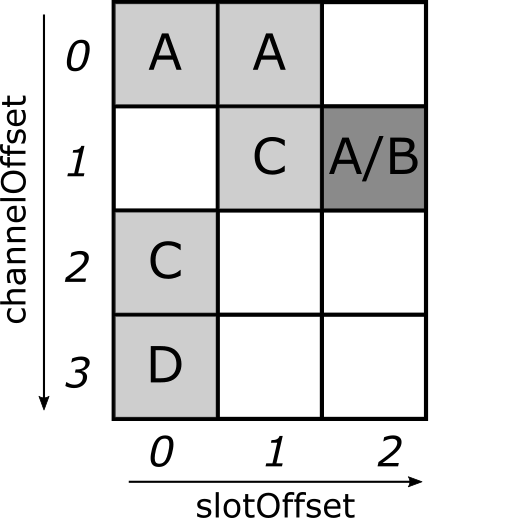
\includegraphics[width=\textwidth]{TSCH_basics_matrix}
		\caption{Exemle de matrice CDU}
		\label{fig:matCDU}
	\end{minipage}\hfill
	\begin{minipage}{0.45\textwidth}
		\centering
		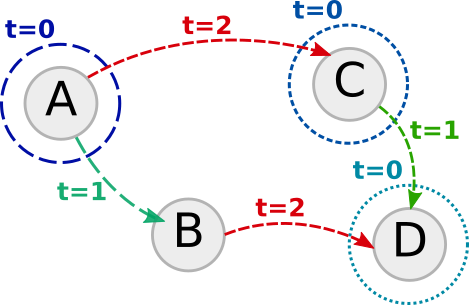
\includegraphics[width=\textwidth]{TSCH_basics_graph}
		\caption{Topolgie d'exemple avec 4 nœuds et leurs transmissions en un cycle de slotframe, détaillées par la \wordlink{Figure}{fig:schedule}}
		\label{fig:topograph}
	\end{minipage}
	\hfill
\end{figure}

\begin{figure}[!h]
	\noindent\makebox[\textwidth]{
		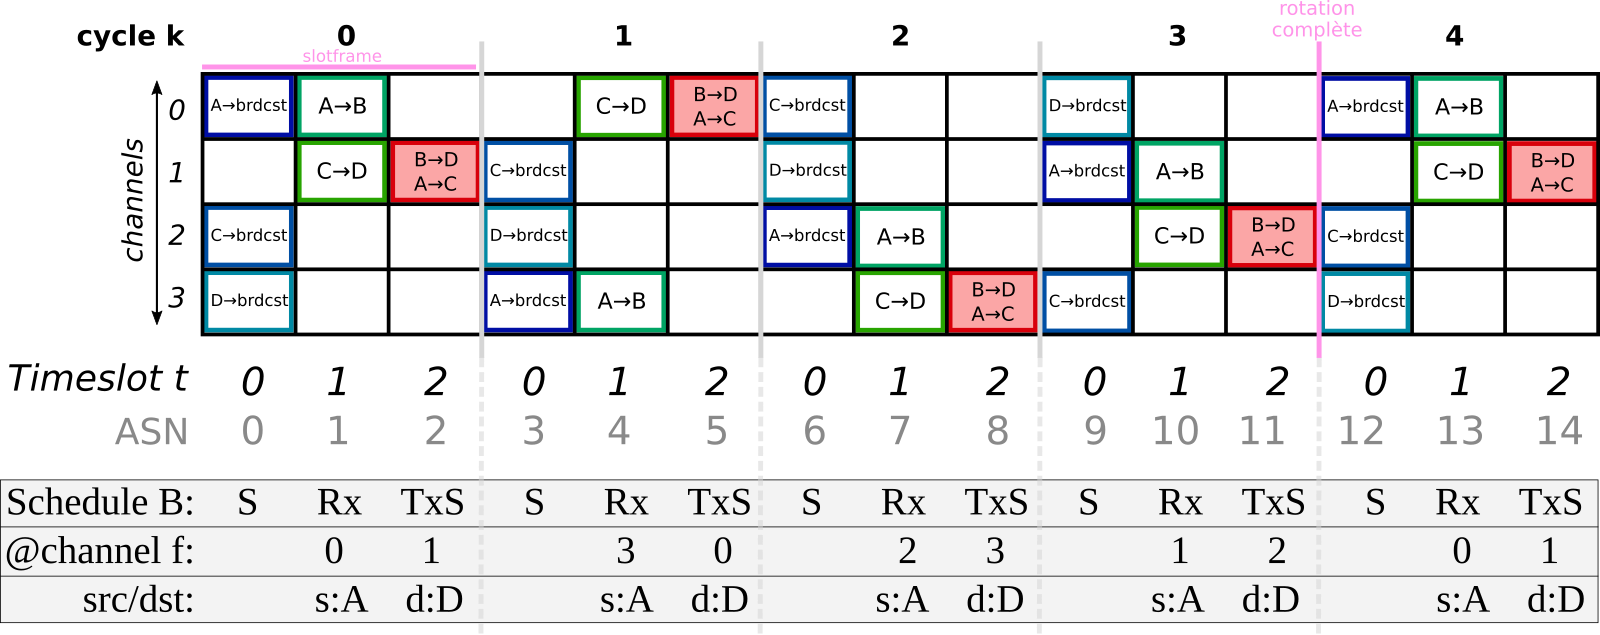
\includegraphics[width=1.1\textwidth]{TSCH_basics_schedule}
	}
		\caption{\textit{Hopping sequences} des transmissions et schedule effectif résultant pour B (slotframes de taille 3)}
		\label{fig:schedule}
\end{figure}

\newpage

Pour exploiter au maximum FDMA et combattre les effets d'interférence/multi-path fading, TSCH utilise un mécanisme de \textit{channel hopping} \cite{rfc7554}. Cela permet d'éviter le fait qu'à chaque cycle d'une slotframe S, une cell qui y est installée (et donc se répète) ne résulte en une transmission ayant lieu à une fréquence identique. Considérant une cell dans le schedule (donc dont on connaît la valeur de channelOffset \textit{chOffset}) et le timeslot courant, cela peut être obtenu simplement avec l'équation suivante :

\begin{align}
f &= F[\: (ASN + chOffset) \quad \text{mod} \ n_{ch} \: ] \\
  &= F[\: ((k \times len(\text{S}) + t) + chOffset) \quad \text{mod} \ n_{ch} \: ] \qquad \text{par \wordlink{l'équation}{ASNeq}}\label{freqeq}
\end{align}

\par Où $n_{ch}$ est le nombre de fréquences considérées pour les transmissions (donc $0 \leq chOffset < n_{ch}$) et $F$ est une fonction bijective qui fait correspondre à un indice de fréquence une valeur réelle parmi celles disponibles (ce qui correspond à utiliser une table de conversion à $n_{ch}$ entrées). En utilisant cette technique, on induit de la variation dans l'usage des fréquences pour une même cell pour des cycles successifs d'une slotframe, et ce malgré le fait que la cell soit statique et dédiée à une transmission de même type. Cependant, le nombre de fréquences disponibles étant borné, ces variations formeront un motif sur plusieurs cycles qui finira par se répéter. Une rotation complète de la \textit{hopping sequence} désigne une itération de ce motif. En analysant \wordlink{l'expression}{freqeq}, on peut facilement déduire que pour maximiser la longueur de ce motif et donc la diversité des fréquences utilisées, on doit avoir que $len(\text{S})$ et $n_{ch}$ sont premiers relatifs \cite{stack-IoT} \cite{rfc7554}. On peut alors considérer qu'il suffit d'utiliser des slotframes de longueur première, le nombre de fréquences $n_{ch}$ n'étant pas un paramètre facilement manipulable. On aura alors une rotation complète après $n_{ch}$ cycles de la slotframe S et la hopping sequence utilisant chacune des $n_{ch}$ fréquences.\\

\par La \wordlink{Figure}{fig:schedule} illustre les hopping sequences des cells installées par chacun des nœuds, c'est-à-dire pour chacune la fréquence à laquelle la transmission aura lieu dans chaque cycle consécutif de la slotframe du nœud. À noter que pour rester concis, on considère ici que $F$ ne renvoie pas des valeurs de fréquence, mais simplement l'identité. On a $len(\text{S}) = 3$ qui est bien premier relatif avec $n_{ch} = 4$, et ce pour la slotframe de chacun des nœuds. Dès lors, on observe bien le phénomène de rotation complétée au cycle 4 qui reprend les même transmissions que le cycle 0. Effectivement, pour chaque cell on observe une hopping sequence couvrant les 4 différentes fréquences disponibles en 4 cycles de slotframe. Le nœud B est choisi arbitrairement pour exhiber un exemple de schedule : durant les 3 timeslots consécutifs de sa slotframe, B va :

\begin{enumerate}
\item Sleep : laisser sa radio éteinte durant la durée du slot
\item Rx : allumer sa radio (sur la fréquence f) et attendre de recevoir une frame de A, et s'il en recoit une valide renvoyer un ACK avant la fin du slot
\item TxS : s'il a une frame destinée à D, allumer sa radio (sur la fréquence f) et utiliser le mécanisme de CSMA/CA pour détecter si le lien est occupé. S'il est libre, il transmet la frame et attend un ACK de D avant la fin du slot
\end{enumerate}

\vspace{0.7cm}

La consommation d'énergie dans un réseau TSCH peut varier en fonction de plusieurs facteurs. La taille des slotframes est le fruit d'un compromis : la diminuer implique qu'un timeslot est davantage répété et donc augmente la bande passante de la transmission associée à la cell qui y est installée, mais entraîne une augmentation de la consommation d'énergie. Un schedule n'est pas forcément statique au cours du temps, des cells peuvent être (dés)installées des slotframes dynamiquement pour correspondre aux besoins d'une application. Cela résulte en une variation de la ``densité" du schedule calculé à partir de ces slotframes : moins il est dense et moins une application dispose de bande passante pour son trafic, mais cela fait également diminuer la consommation énergétique.\\

\newpage

\par TSCH est une collection de concepts permettant des communications efficaces, mais il laisse en suspens plusieurs problèmes que l'implémentation d'une pile réseau basée sur ces concepts devra gérer, notamment :

\vspace{0.2cm}

\begin{itemize}
\item[$\bullet$] la construction, distribution et le maintient (peut-être dynamique) cohérent du schedule des nœuds à travers le réseau pour éviter les inconsistances (voir \wordlink{Section}{scheduling})
\vspace{0.2cm}
\item[$\bullet$] la synchronisation temporelle : les nœuds doivent avoir une notion du temps identique pour commencer leur timeslot au même moment, et ce malgré le phénomène de \textit{clock drifting}. L'ASN maintenu localement par chaque nœud doit également être identique à tout instant pour tous les nœuds d'un même réseau (voir \wordlink{Section}{synchrotemp})
\vspace{0.2cm}
\item[$\bullet$] la formation du réseau : un nouveau nœud le rejoignant n'a aucune connaissance des schedules des autres nœuds, mais doit pouvoir obtenir des cells à hauteur de ses besoins et \textit{in fine} avoir établi son propre schedule et servir à son tour de point d'attache au réseau pour un autre nouveau nœud (voir \wordlink{Section}{joinphase})
\vspace{0.2cm}
\item[$\bullet$] la sécurité à différents niveaux : les hopping sequences (déterministes) restent sujettes aux attaques dites de jamming \cite{R-TSCH} \cite{tiloca-6tisch-robust-scheduling-02}, les opérations d'authentification/chiffrement prennent un temps non négligeable mais doivent tenir intégralement dans un timeslot \cite{link-layer-sec-impact}, la distribution de clés est un problème dans les réseaux restreints \cite{ietf-6tisch-minimal-security-15} \cite{ietf-6tisch-dtsecurity-zerotouch-join-04}, etc.
\end{itemize}

\vspace{0.5cm}

\par La pile 6TiSCH basée sur le mode TSCH de IEEE802.15.4e a pour objectif de standardiser des mécanismes pour apporter une réponse à ces problématiques, la spécification IEEE802.15.4 apportant déjà un canevas pour certaines d'entre elles. Par exemple, le mécanisme de \textit{beacons} annoncés en broadcast pour qu'un nœud puisse rejoindre le réseau en utilisant les informations qu'ils transportent.

\newpage

\chapter{La pile réseau 6TiSCH}
\label{chap_6TiSCH}
\newpage
\section{L'architecture type des WSNs}
\label{archWSN}

	\begin{figure}[!ht]
	\centering
	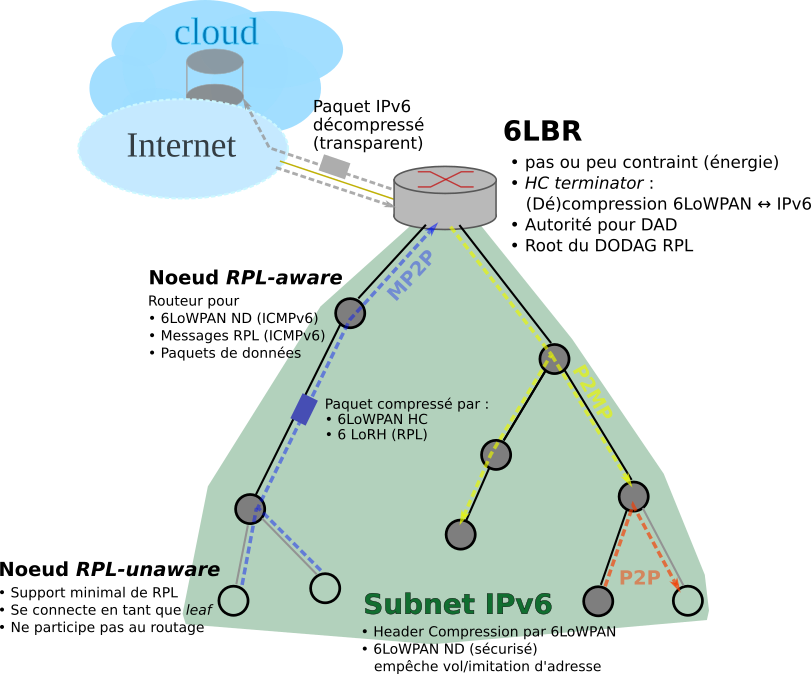
\includegraphics[width=0.9\linewidth]{6TiSCH_arch}
	\caption{Architecture d'un WSN 6TiSCH, calqué sur la configuration basique du standard \cite{ietf-6tisch-architecture-28}}
	\label{fig:archWSN}
	\end{figure}

\vspace{0.2cm}

La \wordlink{Figure}{fig:archWSN} représente un déploiement minimaliste de 6TiSCH dans un seul WSN, désigné par le terme ``sous réseau NBMA" (\textit{Non-Broadcast Multi-Access}) dans la spécification définissant les architectures réseaux 6TiSCH envisageables \cite{ietf-6tisch-architecture-28}. Il en existe des plus complexes supportant la co-existence de plusieurs LLNs le long d'un \textit{backbone} commun, permettant des communications de l'un à l'autre. Les variations dans la conception de tels réseaux reposent notamment sur quels services IPv6 sont mis en place et sur quels équipements. De façon générale, on peut distinguer deux catégories d'équipements dans ces architectures : les nœuds qui font partie intégrante du WSN tels que décrits dans la \wordlink{Section}{WSNs} (donc restreints en ressources) et les équipements qui gèrent le(s) réseau(x) au dessus de la couche lien, avec des services IPv6 ou de routage/scheduling centralisé (NME/PCE (\textit{Path Computing Element})) \cite{ietf-6tisch-architecture-28}.\\

\par Un nœud rejoignant le WSN possède généralement une seule interface radio 802.15.4 à laquelle il doit assigner plusieurs adresses IPv6. Il utilise le mécanisme de \textit{Neighbor Discovery} adapté au réseaux restreints défini par 6LoWPAN ND \cite{rfc6775} \cite{rfc8505}. Le traitement de cette requête de ND diffère en fonction du déploiement des services IPv6, mais elle peut être soit traitée localement par le routeur en bordure du WSN, soit se faire proxy par celui-ci qui la répercutera vers l'ensemble du backbone avec lequel il fait la liaison. Ce routeur porte alors le rôle de 6BBR (\textit{6LoWPAN Backbone Router}) \cite{ietf-6lo-backbone-router-13}. Grâce au mécanisme de 6LoWPAN ND, l'acquisition d'adresse peut se faire de façon sécurisée et garantir l'unicité dans le réseau.

\newpage

\par L'équipement désigné par 6LBR (\textit{6LoWPAN Border Router}) sert de passerelle entre le réseau 6TiSCH et les réseaux extérieurs non restreints, effectuant la traduction entre IPv6 et la couche d'adaptation d'IPv6 aux LLNs, 6LoWPAN (détaillée dans la \wordlink{Section}{6LoWPAN}). Du côté du WSN, le 6LBR est le point d'ancrage de la topologie créée, à savoir le nœud racine du DODAG (\textit{Destination-Oriented Acyclic Graph}) qui est une topologie arborescente maintenue par le protocole RPL (voir \wordlink{Section}{RPL}). Cette structure est donc directement liée à l'utilisation du multi-hop, chaque nœud pouvant communiquer directement (au niveau de la couche lien) avec son parent ou un de ses enfants. Le modèle ainsi défini par RPL permet d'envisager trois types de trafic qui ont des applications typiques \cite{rfc7554} \cite{rfc6550} :\\

\begin{enumerate}
\item MP2P (\textit{Multi-Point to Point}) : un ensemble de nœuds participe à un flux convergeant vers un unique nœud. Par exemple, plusieurs senseurs du WSN effectuent une mesure et transmettent la donnée vers une unité centrale de stockage/traitement située à la bordure ou à l'extérieur du WSN, dans un cloud par exemple (point de collecte généralement désigné par le terme \textit{sink}). Il s'agit d'un flux ascendant vers la racine du DODAG.
\vspace{0.2cm}
\item P2MP (\textit{Point to Multi-Point}) : un nœud génère un flux vers plusieurs autres nœuds. Par exemple, cela peut correspondre à une commande d'action émise depuis la racine du DODAG et destinée à plusieurs actionneurs dans le WSN. Il s'agit d'un flux descendant.
\vspace{0.2cm}
\item P2P (\textit{Point to Point}) : deux nœuds du WSN communiquent point à point. Par exemple, un senseur envoie une mesure à un actionneur qui agit en fonction. Le flux peut emprunter des routes ascendantes et descendantes, mais passera toujours par le plus proche ancêtre commun des deux nœuds.
\end{enumerate}

\newpage

\section{Technologies et protocoles de la pile 6TiSCH}
	\subsection{La pile dans son ensemble}
	\label{6TiSCH_stack}
	
	\begin{figure}[!ht]
	\centering
	\includegraphics[width=0.55\linewidth]{6TiSCH_stack}
	\caption{Pile réseau 6TiSCH proposée par le standard \cite{ietf-6tisch-architecture-28}}
	\label{fig:6TiSCH_stack}
	\end{figure}

\vspace{0.4cm}

La pile illustrée par la \wordlink{Figure}{fig:6TiSCH_stack} reprend les protocoles/concepts considérés comme standards pour la pile 6TiSCH, décrits dans les spécifications écrites par le WG 6TiSCH. Ils sont groupés par correspondance aux couches en utilisant un code couleur, depuis le bas de la pile on a :

\vspace{0.3cm}
\begin{itemize}
\item[$\bullet$] La couche physique (PHY) définie par le standard IEEE802.15.4 réutilisée telle quelle, aucune adaptation n'étant nécessaire pour déployer TSCH par dessus. Voir \wordlink{Section}{802.15.4PHY}.
\vspace{0.2cm}
\item[$\bullet$] La couche lien (MAC) suivant les spécifications du mode TSCH du standard IEEE802.15.4e, qui définit comment \textbf{exécuter} un schedule donné mais pas comment le \textbf{construire}, ni le \textbf{distribuer}. Voir \wordlink{Section}{802.15.4e}.
\vspace{0.2cm}
\item[$\bullet$] La couche d'abstraction de lien et de scheduling qui permet de palier à la problématique de distribution et construction du schedule, tout en définissant une utilisation transparente de celui-ci par la couche réseau (partie du LLC - \textit{Logical Link Control}). Voir \wordlink{Section}{6top}.
\vspace{0.2cm}
\item[$\bullet$] La couche réseau basée sur IPv6 adapté aux réseaux restreints par la couche d'adaptation 6LoWPAN, où RPL est utilisé pour construire la topologie et la maintenir en tenant compte de la nature du réseau. Voir \wordlink{Section}{6LoWPAN} et \wordlink{Section}{RPL}.
\vspace{0.2cm}
\item[$\bullet$] La couche transport, UDP étant utilisé \textit{de facto} préférablement à TCP qui est trop lourd pour des réseaux restreints. Voir \wordlink{Section}{CoAP}.
\vspace{0.2cm}
\item[$\bullet$] La couche application où CoAP est considéré comme un standard adapté à l’interopérabilité avec les réseaux non restreints et servant de base à CoJP (\textit{Constrained Join Protocol}) qui gère le raccord d'un nouveau nœud au WSN, sécurisé à l'aide d'OSCORE (\textit{Object Security for Constrained RESTful Environments}). Voir \wordlink{Section}{CoAP}.
\vspace{0.1cm}
\end{itemize}

\newpage	
	
	\subsection{Couche physique - IEEE802.15.4 PHY}
	\label{802.15.4PHY}

\par La couche PHY sur laquelle 6TiSCH base ses transmissions radios reste inchangée par rapport à celle proposée par la révision du standard IEEE802.15.4 en 2006. Il s'agit d'une technologie radio qui a fait ses preuves, apportant un bon compromis entre la consommation énergétique, la portée et les taux de transmissions possibles à l'échelle de réseaux couvrant la taille d'un immeuble \cite{stack-IoT}. Le standard définit plusieurs PHY, celle adoptée dans le cadre de 6TiSCH opère dans la bande de fréquences 2,4 - 2,485 GHz qui est non licenciée. Cette bande est découpée par le standard en 16 canaux (\textit{channels}) larges de 2 MHz chacun, laissant 5 MHz libres entre deux. Les canaux choisis sont donc orthogonaux, c'est-à-dire ne se recouvrent pas et peuvent donc être utilisés simultanément pour des transmissions différentes. Pour une radio, le changement de canal prend un temps estimé à 192 $\mu s$.\\

\par La technologie de DSSS(\textit{Direct Sequence Spread Spectrum}) est utilisée pour étaler le signal (technique de \textit{spread spectrum}), convertissant un bit de donnée en une séquence de 8 \textit{chips}. Cela permet de réduire les risques d'interférences et d'apporter de la confidentialité si la séquence à la base de l'encodage n'est pas divulguée. Le taux de transmission physique du média étant de 2 Mbps, après étalement le fait de transmettre à 2 Mcps revient à transmettre les données initiales à un débit effectif de 250 kbps. La technique de modulation employée est le O-QPSK (\textit{Offset Quadrature Phase-Shift Keying}), qui utilise des décalages de phases pour encoder l'information.\\

\par Une radio éteinte ne consomme pas de courant, contrairement à une radio allumée qui attend de recevoir, reçoit ou transmets. La consommation est identique, que le nœud soit en attente de réception ou activement en train de recevoir un signal. Comparativement, transmettre coûte généralement un peu plus cher considérant une puissance de 0 dBm (1 mW)\cite{stack-IoT}, mais reste du même ordre de grandeur. Une mesure importante dans l'évaluation de l'efficacité avec laquelle une pile réseau utilise la radio est le \textit{duty cycle}, calculé comme la proportion de temps pendant laquelle la radio reste allumée (Rx et Tx confondus) sur une durée totale. On s'attend à observer un duty cycle inférieur à 1\% dans un WSN déployé avec une pile efficace \cite{stack-IoT}.\\

\par Le standard IEEE802.15.4 définit un schéma de transmission qui est le suivant \cite{stack-IoT} \cite{app-sec-openWSN} :
\vspace{0.2cm}
\begin{itemize}
\item[$\bullet$] Du côté du nœud qui s'apprête à transmettre une frame (voir \wordlink{Figure}{fig:IEEE802.15.4-PHY}) :
	\begin{enumerate}
	\item il émet un préambule de 4 bytes durant 128 $\mu s$ permettant à la radio du receveur de se verrouiller sur le signal de la transmission
	\item le préambule est suivi du SFD (\textit{Start of Frame Delimiter}) de 1 byte indiquant que le début du payload physique vient juste après. Le premier byte de ce payload en indique la taille totale, qui est donc \textbf{limitée à 128-1=127 bytes}.
	\end{enumerate}

\vspace{0.2cm}

\item[$\bullet$] Du côté du nœud qui est maintient sa radio en écoute :
	\begin{enumerate}
	\item il démodule du ``bruit blanc" jusqu'à percevoir le préambule, le reconnaître et se verrouiller dessus
	\item il attend la fin du SFD et considère le byte suivant comme indiquant la longueur du payload physique qui va suivre, allouant donc un buffer de taille suffisante pour y stocker le reste de la frame
	\item une fois le buffer rempli, il indique la réception d'une frame au microcontrôleur en déclenchant une interruption
	\end{enumerate}

\end{itemize}

\vspace{0.8cm}

	\begin{figure}[!ht]
	\centering
	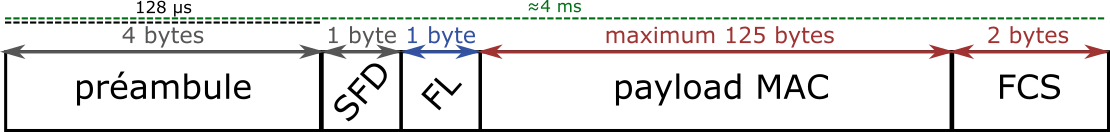
\includegraphics[width=0.9\linewidth]{IEEE802_15_4-PHY}
	\caption{Composants d'une transmission IEEE802.15.4 à la couche PHY. FL pour \textit{Frame Length} et FCS pour \textit{Frame Check Sequence} (somme de contrôle utilisant CRC)}
	\label{fig:IEEE802.15.4-PHY}
	\end{figure}
	
\newpage
	
	\subsection{Couche lien - IEEE802.15.4e en mode TSCH}
	\label{802.15.4e}	

\par Les concepts discutés dans cette section sont décrits formellement dans l'amendement du standard IEEE802. 15.4e de 2011, et maintenus dans sa version plus récente utilisée comme référence par la suite dans ce document : l'IEEE Std 802.15.4-2015 \cite{IEEE802.15.4}. Ce standard ne définit pas \cite{rfc7554} : comment opérer des communications multi-hop, construire et maintenir un schedule, réagir aux changements dans la topologie, gérer les clés de sécurité (génération, (re)distribution), de quelle façon dont un nœud peut rejoindre un réseau en toute sécurité. Ce sont entre autres des fonctionnalités gérées par les couches supérieures, présentées dans le reste de ce chapitre.
	
\subsubsection{Structure de PAN et addressage}

On considère le réseau comme un LR WPAN (\textit{Low Rate Wireless Personal Area Network}), équivalent à un WSN et où le standard distingue deux types de nœuds : les FFDs (\textit{Full Function Devices}) et les RFDs (\textit{Reduced Function Devices}). Les premiers sont des nœuds peu ou pas contraints en ressources, capables d'endosser les rôles de \textit{PAN coordinator}, \textit{simple coordinator} ou encore de simple nœud. Les seconds sont de simples nœuds limités en ressources, ils ne peuvent pas assumer les tâches d'un FFD qui sont entre autres la coordination entre PANs (pour un PAN coordinator), l'allocation d'adresse, la gestion du canal et l'émission régulière de \textit{beacons} avertissant la présence du réseau pour de nouveaux nœuds. Les topologies formées par ces nœuds peuvent être adaptées en fonction des besoins, celles utilisées communément sont illustrées par la \wordlink{Figure}{fig:PANs} (TSCH reste applicable dans tous les cas \cite{IEEE802.15.4}) :
\vspace{0.2cm}
\begin{itemize}
\item[a.] Topologie en étoile autour d'un coordinator, toute communication ayant lieu avec lui
\vspace{0.1cm}
\item[b.] Topologie \textit{peer-to-peer} où les communications ont lieu entre RFD et coordinators, ces derniers pouvant communiquer entre eux et avec le PAN coordinator faisant le lien avec d'autres PANs
\vspace{0.1cm}
\item[c.] Topologie \textit{ad-hoc} entre RFDs, sans coordinator pour gérer les communications
\end{itemize}

\vspace{0.4cm}

	\begin{figure}[!ht]
	\centering
	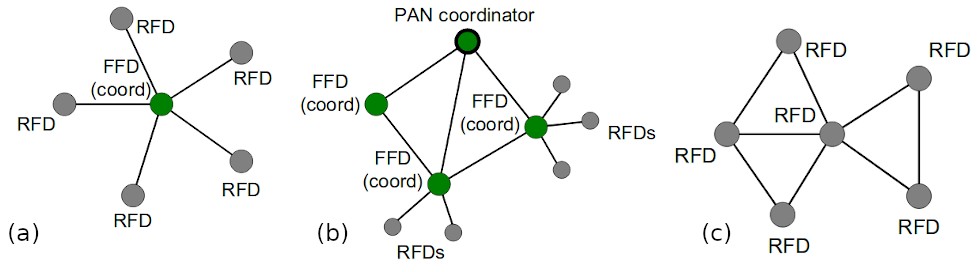
\includegraphics[width=0.9\linewidth]{PANs}
	\caption{Différentes structures envisageables et combinables pour un PAN IEEE802.15.4}
	\label{fig:PANs}
	\end{figure}

\vspace{0.2cm}

\par À un PAN créé correspond un PAN ID supposé unique parmi les PANs à portée du nœud qui l'initialise. Chaque nœud dans ce PAN peut utiliser une adresse de 64 bits (dérivée par EUI-64 \cite{IEEE802.15.4}) dite \textit{extended}, notamment avant de l'avoir totalement rejoint. Une fois accepté par un coordinator, un nœud se voit allouer par celui-ci une \textit{short address} de 16 bits dont le champ d'action est limité au PAN (si elle est utilisée seule). Un nœud dans un autre PAN peut être atteint en utilisant une combinaison de sa short address et de l'ID de ce PAN. Une frame 802.15.4 peut donc être adressée en utilisant une combinaison de modes d'adresses (champs destination et source décrits chacun par [PAN ID+short address] ou [extended address]). Un schéma récapitulant le contenu et le format d'une frame 802.15.4e, considérant également les éléments détaillés dans sections suivantes, est donné par la \wordlink{Figure}{fig:IEEE802.15.4_frame}.

\newpage

\subsubsection{IEs et \textit{Enhanced Beacons}}
\label{EBs}

L'amendement IEEE802.15.4e a amené le concept d'IE (\textit{Information Element}) dans les champs facultatifs des frames. Un IE est un conteneur composé des champs \textit{Type-Length-Value}, placé à la fin du header MAC classique. Un bit dans le header MAC indique si une frame contient des IEs. Ceux-ci sont groupés en deux types : les \textit{Headers IEs}, consommés à la couche MAC et invisibles pour les couches supérieures et les \textit{Payload IEs}, passés tels quels aux couches supérieures. Les Headers IEs sont placés à la fin du header MAC (et en font partie), les Payload IEs sont placés juste après, avant le payload MAC (et en font partie). Les Payload IEs servent donc à échanger des informations structurées entre nœuds voisins, permettant une extensibilité du standard. TSCH utilise des nouveaux IEs pour étendre le standard 802.15.4 \textit{legacy}.\\

\par Comme détaillé dans la \wordlink{Section}{joinphase}, la formation du réseau s'opère par le broadcast de frames spéciales de signalement, émises par les nœuds déjà membres du réseau. Ces frames, appelées \textit{beacons}, ont fait l'objet d'adaptations au mode TSCH afin d'annoncer les informations qu'il requiert sous la forme d'IEs. Les frames améliorées en résultant sont appelées EBs (\textit{Enhanced Beacon}), elles présentent au minimum les caractéristiques suivantes selon le standard \cite{IEEE802.15.4} :
\vspace{0.2cm}
\begin{itemize}
\item[$\bullet$] adresse destination mise à \texttt{0xFFFF} (short broadcast) et adresse source à la short address du nœud annonceur, ou extended si cette dernière n'est pas définie
\vspace{0.1cm}
\item[$\bullet$] non-ACKable, aucun ACK ne doit être renvoyé après réception d'un EB
\vspace{0.1cm}
\item[$\bullet$] IE \textit{TSCH Synchronization} : informations concernant l'ASN courant et la \textit{Join Metric}
\item[$\bullet$] IE \textit{TSCH Timeslot} : identifiant du template de timeslot qui organise les timings des actions internes effectuées durant un timeslot (\wordlink{Section}{templatetimeslot})
\item[$\bullet$] IE \textit{Channel Hopping} : identifiant de la la séquence de fréquences utilisée pour la conversion d'un channel offset vers un numéro de canal (ie. fréquence réelle utilisée)
\item[$\bullet$] IE \textit{TSCH Slotframe and Link} : renseigne au nœud rejoignant le réseau un schedule initial minimal pour y communiquer, \cite{rfc8180} recommande une seule cell, typée RxTxS (voir point suivant)
\end{itemize}


\subsubsection{Types de transmissions et retransmissions}

\par Une transmission à la couche lien peut être broadcast (EBs principalement, à l'adresse dédiée \texttt{0xFFFF}) ou unicast (paquets de données, à l'adresse short préférentiellement à l'extended). Elle peut demander le renvoi d'un ACK à la bonne réception de la frame ou un NACK si elle a bien été reçue mais que son traitement a résulté en une erreur (sécurité notamment), ou ne rien attendre en retour. Le mode TSCH associe chaque transmission à une cell, la cell étant paramétrée pour correspondre à l'action voulue.\\

\par Une cell peut être déclarée \textit{dedicated} ou \textit{shared} (S). Étant \textbf{dedicated}, un nœud considère que le lien derrière la cell n'est utilisé que par lui et n'emploie pas le CCA (\textit{Clear Channel Assessment}) pour s'assurer que le canal est libre avant de transmettre. Étant \textbf{shared}, une cell est susceptible de servir pour des transmissions simultanées, CCA est donc employé et la transmission est lancée uniquement si le canal est libre, sinon elle est différée à une prochaine cell valide pour l'envoi de la frame. Une cell active (non considérée comme \textit{Sleep}) est associée à un rôle dans la communication : réception d'une frame (\textbf{Rx}), envoi d'une frame (\textbf{Tx}) ou les deux en même temps (\textbf{RxTx}). Cela correspond aux comportements suivants :
\vspace{0.2cm}
\begin{itemize}
\item[$\bullet$] Rx : le nœud passe sa radio en écoute après un temps déterminé depuis le début du slot et attend de capter le préambule d'une frame pendant une courte période. Si rien n'est reçu, la radio est éteinte. Si une frame arrive durant cette période, qu'elle n'est pas jetée par le nœud (dst correspondante, sécurité, etc.) et qu'un ACK est demandé, alors celui-ci est construit et renvoyé avant la fin du slot.
\vspace{0.1cm}
\item[$\bullet$] Tx : le nœud regarde s'il a une frame dans sa queue correspondant au destinataire de la cell, sinon il laisse sa radio éteinte pour le reste du slot. S'il en a une, il la transmet et passe ensuite sa radio en écoute pour le reste du slot si elle demande un ACK.
\vspace{0.1cm}
\item[$\bullet$] RxTx : prend le comportement de Tx s'il y a une frame correspondante dans la queue, sinon prend le comportement de Rx. Si la cell est également Shared (S), le comportement résultant est similaire à du Slotted-Aloha \cite{rfc7554}.
\vspace{0.1cm}
\end{itemize}

\newpage

\par Les transmissions Tx peuvent utiliser le mécanisme de CCA pour éviter les collisions qui se produisent même dans TSCH (proximité d'autre réseau, schedule inconsistant), ou l'ignorer et transmettre d'office la frame, en fonction d'un paramètre booléen \textit{TschCca} \cite{IEEE802.15.4}. Le fait de différer l'envoi d'une frame suite à la détection de l'occupation du canal par CCA n'est pas considéré comme une retransmission. En revanche, lorqu'une frame requérant un ACK est effectivement transmise et que ce dernier n'est jamais reçu en retour, une retransmission devra avoir lieu dans une cell future qui soit valide pour cette frame.\\

\par Pour éviter les phénomènes de collisions successives répétées, la sélection de cette cell est basée sur l'algorithme de \textit{random backoff} CSMA-CA. Il choisira aléatoirement une cell dans d'une certaine fenêtre, celle-ci grandissant au fur et à mesure des échecs de retransmissions sur un même lien. Il s'agit donc d'un \textit{backoff} ``discret", en terme de timeslots à écouler. Le paramètre BE (\textit{backoff exponent}) régule cette taille de fenêtre et n'est incrémenté/réinitialisé que quand la (re)transmission a lieu dans une cell shared correspondant au même lien (vers le même voisin). Il est cependant réinitialisé dans le cas où une retransmission est réussie sur le même lien depuis une cell dedicated et que la queue est vide. La \wordlink{Figure}{fig:CSMA} schématise le système de (re)transmission quand on considère que CCA est utilisé avant toute (re)transmission. Passés un certain nombre d'essais, 3 retransmissions étant la valeur conseillée par le standard \cite{IEEE802.15.4}, la frame est jetée et les couches supérieures en sont notifiées.

	\begin{figure}[!ht]
	\centering
	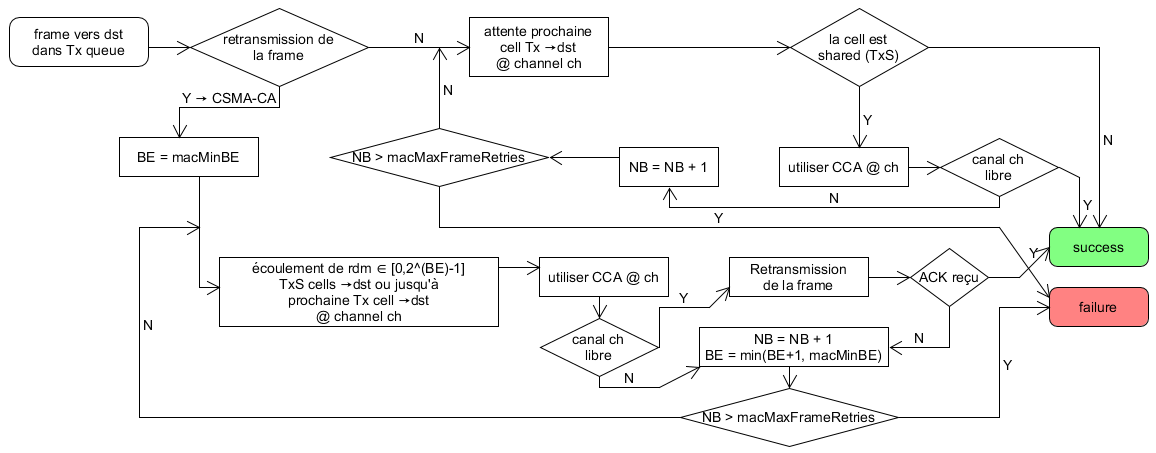
\includegraphics[width=0.9\linewidth]{CSMA-CA}
	\caption{Déroulement de la (re)transmission d'une frame destinée au nœud dst considérant \textit{TschCca=ON}}
	\label{fig:CSMA}
	\end{figure}


\subsubsection{Organisation d'une transmission dans un timeslot}
\label{templatetimeslot}

\par Une cell active se traduit en un timeslot dans lequel un nœud aura le rôle de Transmitter (Tx) et l'autre le rôle de Receiver (Rx). En un seul timeslot, si le Transmitter a une frame à destination du Receiver, elle doit être transmise intégralement et l'ACK correspondant, si demandé, doit être renvoyé avant la fin du timeslot. Selon \cite{rfc7554} et \cite{ATP}, on a au maximum 127+6 bytes pour les parties PHY et MAC de la frame envoyée, ce qui prend approximativement 4ms et l'ACK en retour prend de l'ordre de 1ms. Bien que les nœuds soient synchronisés en terme de timeslots (même ASN), ils peuvent avoir une perception légèrement différente du temps courant à cause du phénomène de \textit{clock drifting}, dû aux imperfections des cristaux et aux différences de températures \cite{vulns-time-synchro-TSCH}. Par conséquent, ils ne commencent pas leur timeslot exactement au même moment et une marge d'erreur doit être considérée. L'idée est de planifier la transmission à un instant précis du timeslot connu des deux nœuds, mais le Receiver allumera sa radio dans une fenêtre de temps autour de cet instant. Il anticipe ainsi le fait que sa perception du temps le place comme en avance ou en retard par rapport au Transmitter. La différence de perception peut être corrigée régulièrement par des mécanismes de resynchronisation décrits à la \wordlink{Section}{synchrotemp}.\\

\newpage

\par La démarche adoptée est la séquentiation d'un timeslot en périodes de temps discrètes, de longueur déterminée en fonction du rôle joué dans la communication. Ces périodes ont chacune un rôle particulier, définies par un nom et une valeur en $\mu s$. Un ensemble formé par ces périodes avec des valeurs données est appelé \textit{timeslot template}, auquel est associé un ID unique. Tous les nœuds d'un réseau TSCH doivent être alignés sur un même template, celui-ci étant communiqué aux nœuds dans l'IE \textit{TSCH Timeslot} des EBs. Le standard \cite{IEEE802.15.4} définit un template par défaut associé à l'ID \texttt{0x00}, que chaque nœud devrait connaitre (évitant la transmission des 25 bytes d'IE pour un template personnalisé). Il considère une longueur totale de slot \textit{macTsTimeslotLength} de 10 ms. La \wordlink{Figure}{fig:timeslot} en schématise l'exécution :
\vspace{0.2cm}
\begin{itemize}
\item[$\bullet$] Du côté du Transmitter :
\begin{enumerate}
\item Il débute le slot en appliquant CCA et, s'il ne doit pas différer la transmission, il passe sa radio en mode émission, commençant à transmettre la frame après exactement \textit{macTsTxOffset} $\mu s$ par rapport au début du slot.
\vspace{0.1cm}
\item Une fois la frame entièrement transmise, il attend \textit{macTsRxAckDelay} $\mu s$ (temps dédié au traitement de la frame et construction de l'ACK par le Receiver) et passe sa radio en mode écoute.
\vspace{0.1cm}
\item Il attend l'ACK \textit{macTsAckWait} $\mu s$, s'il n'arrive pas dans dans ce délai, la transmission est considérée comme un échec et le mécanisme de retransmission peut être utilisé.
\end{enumerate}
\vspace{0.1cm}
\item[$\bullet$] Du côté du Receiver :
\begin{enumerate}
\item Il allume sa radio \textit{macTsRxOffset} = $macTsTxOffset - \frac{macTsRxWait}{2} \; \mu s$ après le début du slot, laissant alors une fenêtre de temps de \textit{macTsRxWait} $\mu s$ pour commencer à recevoir la frame. Si rien n'est reçu passé ce délai, il éteint sa radio pour le reste du slot.
\vspace{0.1cm}
\item Une fois la frame reçue dans son intégralité, il laisse s'écouler un délai de \textit{macTsTxAckDelay} $\mu s$ durant lequel il traite la frame, construit l'ACK et passe sa radio en mode émission.
\vspace{0.1cm}
\item Il transmet l'ACK résultant et éteint sa radio.
\end{enumerate}
\end{itemize}
	
\vspace{0.4cm}	
	
\par La valeur de \textit{macTsRxOffset} définit la fenêtre de temps considérée pour palier à la désynchronisation des nœuds. Le fait de la fixer à \textit{macTsTxOffset} $- \frac{macTsRxWait}{2} \: \: \mu s$ permet d'absorber une différence de perception entre les horloges jusqu'à $\frac{macTsRxWait}{2} \;\mu s$ \cite{ATP}. Si les horloges étaient parfaitement synchronisées, le Receiver pourrait s'attendre à recevoir la frame exactement \textit{macTsRxOffset} $+ \frac{macTsRxWait}{2} \; \mu s$ après le début du timeslot. Le standard \cite{IEEE802.15.4} donne pour le template \texttt{0x00} les valeurs suivantes : \textit{macTsTxOffset} à 2120 $\mu s$ et \textit{macTsRxWait} à 2200 $\mu s$. Les horloges ne peuvent donc pas être désynchronisées de plus de 1100 $\mu s$, sinon la transmission échouera.

\vspace{0.4cm}

	\begin{figure}[!ht]
	\centering
	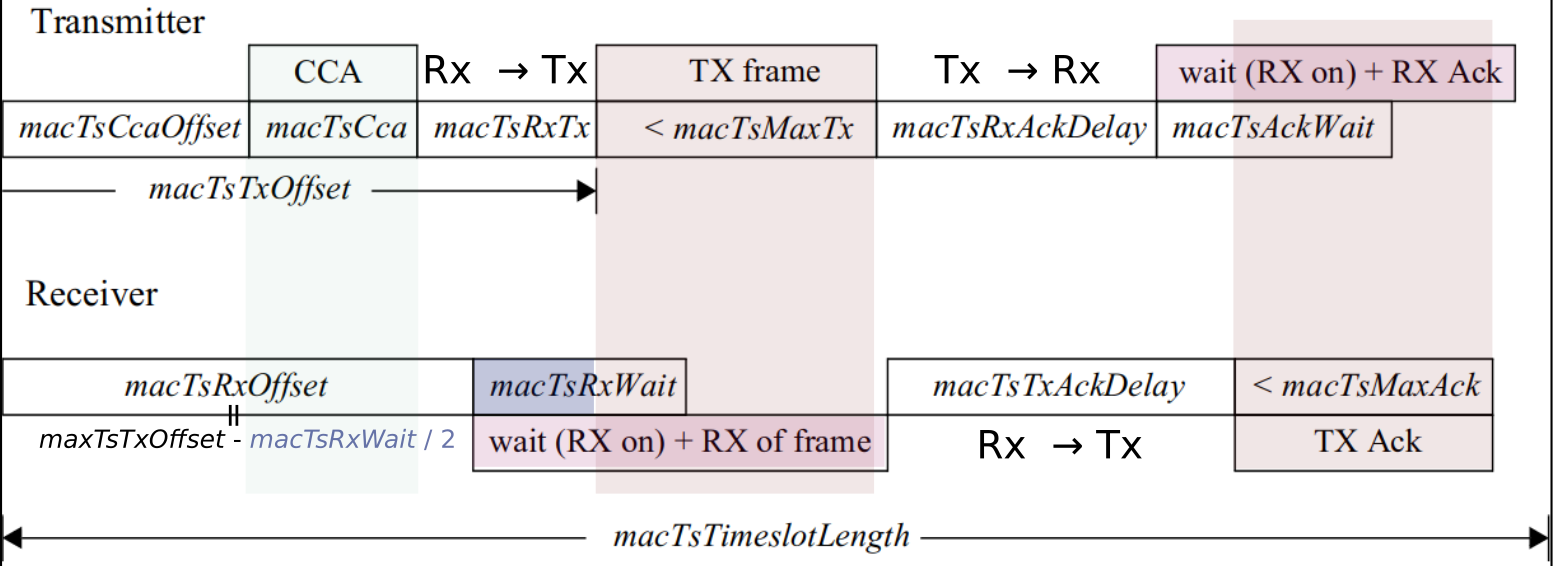
\includegraphics[width=\linewidth]{timeslot}
	\caption{Utilisation des différentes périodes délimitées dans un timeslot lors d'une transmission}
	\label{fig:timeslot}
	\end{figure}

\subsubsection{Services de sécurité}
\label{IEEE802.15.4-sec}

Des mécanismes de sécurisation des communications à la couche 2 ont été prévus dans le standard pour assurer la confidentialité, l'authentification et l'intégrité des transmissions. L'algorithme considéré est AES, généralement avec une clé de 128 bits, car il est un bon compromis entre la taille du code, les performances en temps et la solidité apportée, en plus de bénéficier d'un port hardware \cite{link-layer-sec-impact}. Il s'agit donc d'un chiffrement symétrique pour lequel les nœuds doivent posséder la même clé afin de se comprendre, ce qui implique une notion de distribution du matériel de \textit{keying} non décrite dans le standard \cite{IEEE802.15.4}.\\

\par Le schéma considéré est CCM* qui est un \textit{wrapper} autour des primitives AES pour sécuriser une frame avec une clé donnée (\wordlink{Figure}{fig:CCM}). En arrière-plan, l'authentification d'une frame entière se fait par le mode CBC-MAC (\textit{Cipher Block Chaining}-\textit{Message Authentication Code}) et le chiffrement par le mode CTR (\textit{CounTeR}). Le premier va générer un hash sur la frame entière (aussi appelé MIC - \textit{Message Integrity Code}) qui est tronqué et ajouté à la fin de la frame, recalculable par le Receiver s'il a la clé et la frame. Le second permet de chiffrer le contenu du paquet (Payload IEs et payload de la frame) à partir d'une clé et d'un compteur commun entre les parties communiquantes dit \textit{nonce}, qui est \textit{macAsn} dans le cas de TSCH.\\

\par Huit niveaux de sécurité sont distingués par le standard, en fonction de la longueur désirée du MIC et de l'usage du chiffrement. Chaque nœud maintient une table \textit{macKeyTable} dont les entrées sont des conteneurs \textit{KeyDescriptors} contenant entre autres la valeur de la clé, quels autres nœuds peuvent l'utiliser, sa source \textit{KeySource}, son index \textit{KeyIndex}. À chaque frame sécurisée, le nœud rajoute un ASH (\textit{Auxiliary Security Header}) juste après le header MAC (voir \wordlink{Figure}{fig:IEEE802.15.4_frame}), indiquant quel est le niveau de sécurité à considérer et quelle clé employer en fournissant le couple (\textit{KeySource, KeyIndex}). La taille de l'ASH varie entre 5 et 14 bytes, bien que celui-ci puisse omettre le \textit{Frame Counter} en mode TSCH (l'ASN fait en partie office de nonce).

\vspace{0.2cm}

	\begin{figure}[!ht]
	\centering
	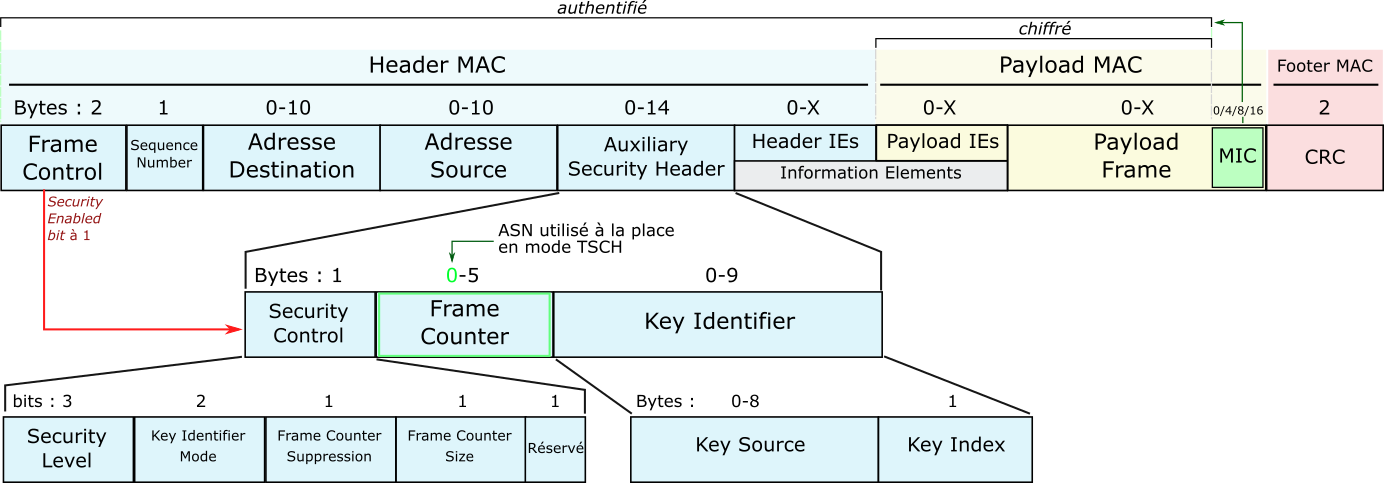
\includegraphics[width=\linewidth]{IEEE802_15_4-MAC}
	\caption{Structure d'une frame 802.15.4e selon le standard \cite{IEEE802.15.4}}
	\label{fig:IEEE802.15.4_frame}
	\end{figure}


	\begin{figure}[!ht]
	\centering
	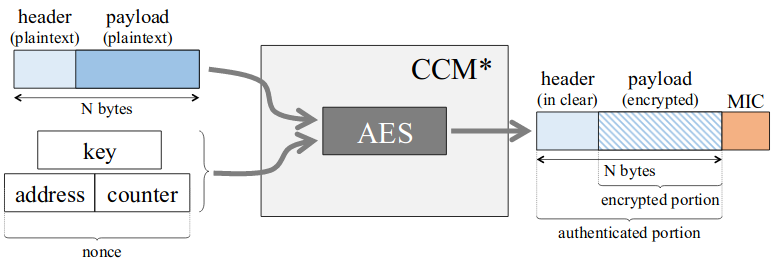
\includegraphics[width=0.7\linewidth]{CCM}
	\caption{CCM* permet de chiffrer/authentifer des frames à partir d'une clé \cite{link-layer-sec-impact}}
	\label{fig:CCM}
	\end{figure}

\newpage


\subsubsection{Structure de slotframe}

Le standard IEEE802.15.4-2015 \cite{IEEE802.15.4} reprend les notions théoriques de TSCH présentées à la \wordlink{Section}{tschfond}. Un nœud maintient une table \textit{macSlotframeTable} dont les entrées sont composées d'un identificateur de slotframe \textit{macSlotframeHandle} et de la taille \textit{macSlotframeSize} de cette dernière. Il maintient également une table \textit{macLinkTable} qui correspond à l'ensemble des cells utilisées par le nœud (terme interchangeable avec \textit{link}), chaque entrée possédant des attributs tels que l'indentificateur de la slotframe où elle est installée, son type (Rx, RxS, etc.), l'adresse du nœud à l'autre extrémité du lien et les coordonnées de la cell \textit{macTimeslot} et \textit{macChannelOffset}. Un compteur global \textit{macAsn} est incrémenté toutes les \textit{macTsTimeslotLength} $\mu s$.\\

\par La co-existence de plusieurs slotframes est donc envisagée par le standard. Comme le nœud n'a qu'une radio, il ne peut considérer qu'une seule cell par timeslot. Des règles de précedences sont donc établies pour pouvoir départager des cells concurrentes :
\vspace{0.1cm}
\begin{enumerate}
\item une transmission (Tx) est prioritaire sur une réception (Rx)
\vspace{0.1cm}
\item une slotframe avec une valeur de \textit{macSlotframeHandle} plus petite est prioritaire (et par extension les cells qui y sont installées)
\end{enumerate}


\subsubsection{Table des voisins}
\label{neighbors_table}

Chaque nœud maintient une liste \textit{secDeviceList} des voisins avec qui il peut communiquer de manière sécurisée, sous la forme de \textit{secDeviceDescriptors}, chacun stockant les attributs suivants :
\vspace{0.2cm}
\begin{itemize}
\item[$\bullet$] \textit{secPanId} : l'identificateur du PAN auquel appartient le nœud
\vspace{0.1cm}
\item[$\bullet$] \textit{secShortAddress} : la short address du nœud, ou la valeur \texttt{0xFFFE} s'il utilise uniquement son extended (\texttt{0xFFFF} pour inconnue)
\vspace{0.1cm}
\item[$\bullet$] \textit{secExtAddress} : l'extended address du nœud
\vspace{0.1cm}
\item[$\bullet$] \textit{secExempt} : booléen indiquant si le nœud peut ignorer la valeur du paramètre de niveau de sécurité minimum, c'est-à-dire que les frames originaires de ce nœud peuvent être acceptées quelque soit le niveau de sécurité considéré pour les sécuriser
\vspace{0.1cm}

\end{itemize}

\newpage

	\subsection{Couche d'abstraction de lien - 6top}
	\label{6top}

\subsubsection{Composants de la couche 6top}

\par 6top (\textit{6TiSCH Operation sublayer}, \cite{rfc8480}) est une couche intermédiaire introduite par le WG 6TiSCH pour apporter des services requis par le déploiement d'un réseau TSCH basé sur la couche MAC 802.15.4. 6top peut être considéré comme une sous-couche dans les services qui devraient être offerts par la couche intermédiaire de LLC (\textit{Link Layer Control}). La spécification \cite{rfc7554} fait l'état de tous les services que l'entité fonctionnelle LLC devrait supporter dans un réseau TSCH, parmi ceux-ci 6top contribue aux points :

\vspace{0.2cm}

\begin{itemize}
\item[$\bullet$] 3.5. \textit{Resource Management} : les cells TSCH constitue des ressources unitaires à distribuer entre les nœuds du réseau, deux voisins souhaitant communiquer le font par le biais de la même cell (installée comme Tx pour l'un et Rx pour l'autre). 6top permet la négociation distribuée et autonome des cells entre voisins à travers le protocole 6P (\textit{6top Protocol}). 6top peut également servir d'interface à une entité centralisée (PCE, ...) pour prendre la main dans la configuration des schedules.
\vspace{0.2cm}
\item[$\bullet$] 3.8 \textit{Scheduling Mechanisms} : les variations de trafic entre nœuds sont courantes, aussi un schedule efficace est un schedule capable de s'adapter dynamiquement. Un mécanisme de surveillance de l'état des communications et de régulation des schedules par (dés)allocation subséquente de cells est mis en place au travers du concept de SF (\textit{Scheduling Function}). À chaque application du réseau peut correspondre une SF, 6top gère leur exécution simultanée qui est prise en compte de façon transparente par 6P.
\end{itemize}

\vspace{0.6cm}

\par La couche 6top permet d'établir une abstraction des couches plus basses, de sorte que les couches supérieures ne doivent pas opérer avec 6top explicitement en terme de cell (couples (slotOffset, channelOffset)). À la place, les requêtes vers 6top devraient s'effectuer en terme de bande passante et QoS demandées pour un \textit{bundle} de cells, un bundle étant un ensemble de cells d'une même nature (type et autre extrémité du lien) et donc interchangeables. Une ``API" assure l'interfaçage avec ce niveau d'abstraction, la transformation en terme de cell et la négociation de leur (dés)allocation avec le voisin concerné étant invisible pour la couche supérieure qui présente sa requête \cite{ietf-6tisch-architecture-28}. Pour promouvoir l'adaptation dynamique du schedule, 6top maintient une \textit{abstract neighbor table} dont chaque entrée correspond à un voisin, stockant des mesures relatives aux communications avec ce dernier : RSSI\footnote{\url{https://fr.wikipedia.org/wiki/Received_Signal_Strength_Indication}}/LQI\footnote{\url{https://www.sciencedirect.com/topics/engineering/link-quality}} de chaque cell, timestamp du dernier paquet, nombre de paquets envoyés et reçus, etc. \cite{ietf-6tisch-architecture-28}. Ces informations peuvent également être accédées en passant par l'API de 6top, utilisées par exemple par l'\textit{Objective Function} de RPL pour calculer un rang (voir \wordlink{Section}{RPL}).\\

\par 6top permet donc la co-existence de plusieurs entités agissant sur le schedule : dispositif centralisé  de calcul des routes (PCE), SFs adaptant dynamiquement le schedule en fonction des applications et donc potentiellement aussi nombreuses et variées que ces dernières. Afin d'éviter les conflits entre ces sources, 6top différencie les \textit{hard/soft} cells :

\vspace{0.2cm}

\begin{itemize}
\item[$\bullet$] Une hard cell est une cell ``hard-codée" ou installée par une entité extérieure (PCE) pour ses besoins (\textit{forwarding} déterministe par exemple), sans passer par la couche d'abstraction. Ces cells ne devraient pas être manipulées par 6top, elles sont donc en lecture seule de son point de vue. Le standard \cite{rfc8480} préconise l'usage d'une slotframe dédiée à ces cells, d'identificateur minimal par rapport aux autres slotframes de sorte à ce qu'elles aient toujours la priorité.
\vspace{0.2cm}
\item[$\bullet$] Une soft cell est gérée localement par 6top. Une couche supérieure passant par l'API pour faire sa requête ne donne pas de cell concrète, c'est 6top qui se chargera de la sélection et manipulation de soft cells précises. Une SF qui détecte un besoin de changement dans le schedule pour s'adapter au trafic utilisera également des soft cells dans ses négociations par le protocole 6P.
\end{itemize}

\vspace{0.6cm}

\par Malgré ces dispositions, des collisions de schedule restent encore possibles \cite{ietf-6tisch-architecture-28}. Effectivement, le fait que 6top considère une négociation distribuée de voisin à voisin ne garantit pas une consistance globale de l'allocation des soft cells.

\newpage

\subsubsection{Le protocole 6P et les scheduling functions}

\par 6P permet à un nœud de communiquer avec son voisin pour négocier l'ajout/la suppression/le déplacement de cell dans leur schedule de façon consistante. Il s'agit donc d'une négociation distribuée sous la forme de \textit{Transaction} entre nœuds voisins. Une Transaction est initiée par un message formaté de type \textit{Request}, sous impulsion d'une SF qui détecte un besoin d'adaptation du schedule au trafic. Une Transaction s'opère dans une optique de négociation, aussi on a toujours un schéma calqué sur une proposition d'un nœud suivie d'une confirmation de ce qui convient à l'autre nœud qui la reçoit. Un échange 6P se fait préférentiellement en employant une cell dedicated entre deux voisins (\textit{single hop}) et est totalement encapsulé dans un Payload IE (IE 6top de format générique gérant tous les messages).\\

\par Deux types de Transactions sont envisagés par 6P en fonction de quel nœud sera celui qui fait la proposition : on différencie des Transactions \textit{2-steps} et \textit{3-steps}. Trois types de messages sont échangés lors des Transactions : \textit{REQUEST}, \textit{RESPONSE} et \textit{CONFIRMATION}. Par Transaction, un unique type de cell \textit{CellOptions} est considéré, s'appliquant en fonction de la sémantique de la commande associée (ajout/suppression/déplacement de cell entre autres). Par exemple, une commande ADD accompagnée de CellOptions indiquant ``Rx" va résulter en l'installation de cell(s) dans les schedules des deux nœuds, de type Rx pour le nœud à l'origine de la Request et Tx pour l'autre. Les principales commandes sont ADD, DELETE, RELOCATE, COUNT et LIST. À tout message 6top sont associés un SFID (\textit{SF Identificator}) et un numéro de séquence \textit{SeqNum}. Le premier permet d'identifier quelle SF doit traiter la Transaction, plusieurs SFs pouvant co-exister. Le second est utilisé pour faire correspondre les messages REQUEST/RESPONSE/CONFIRMATION et maintenir un état consistant entre les schedules impactés. Les Figures \ref{fig:2-steps} et \ref{fig:3-steps} illustrent respectivement une commande ADD orchestrée en 2 et 3-steps, avec les périodes durant lesquelles des cells sont ``verrouillées" afin de maintenir un état consistant jusqu'à la fin de la Transaction qui valide définitivement leur installation.\\

\par Pour pouvoir négocier, deux nœuds doivent faire tourner la même SF. Le traitement des messages 6P reçus est redirigé vers la bonne SF en fonction du SFID contenu dans le message. Pour permettre les communications arbitraires entre même SFs d'un nœud à l'autre, 6top inclut un champ \textit{Metadata} dans certaines commandes (16 bits) et une commande dédiée SIGNAL. Par exemple, le champ Metadata d'une commande ADD peut indiquer la slotframe dans laquelle installer les cells. La valeur est passée telle quelle à la SF, comme c'est également le cas pour les champs CellOptions (bitmap de 8 bits) et CellList (liste de cells représentées sur 4 bytes, 2/2 pour slotOffset/channelOffset). Ces derniers sont des paquets de bits opaques formatés par la SF, les contenus indiqués ici étant recommandés par le standard \cite{rfc8480}. Une SF doit également gérer la détection et le traitement d'inconsistances, les erreurs renvoyées lors d'une Transaction et les valeurs de timeouts.

\begin{figure}[!ht]
	\centering
	\begin{minipage}{0.5\textwidth}

		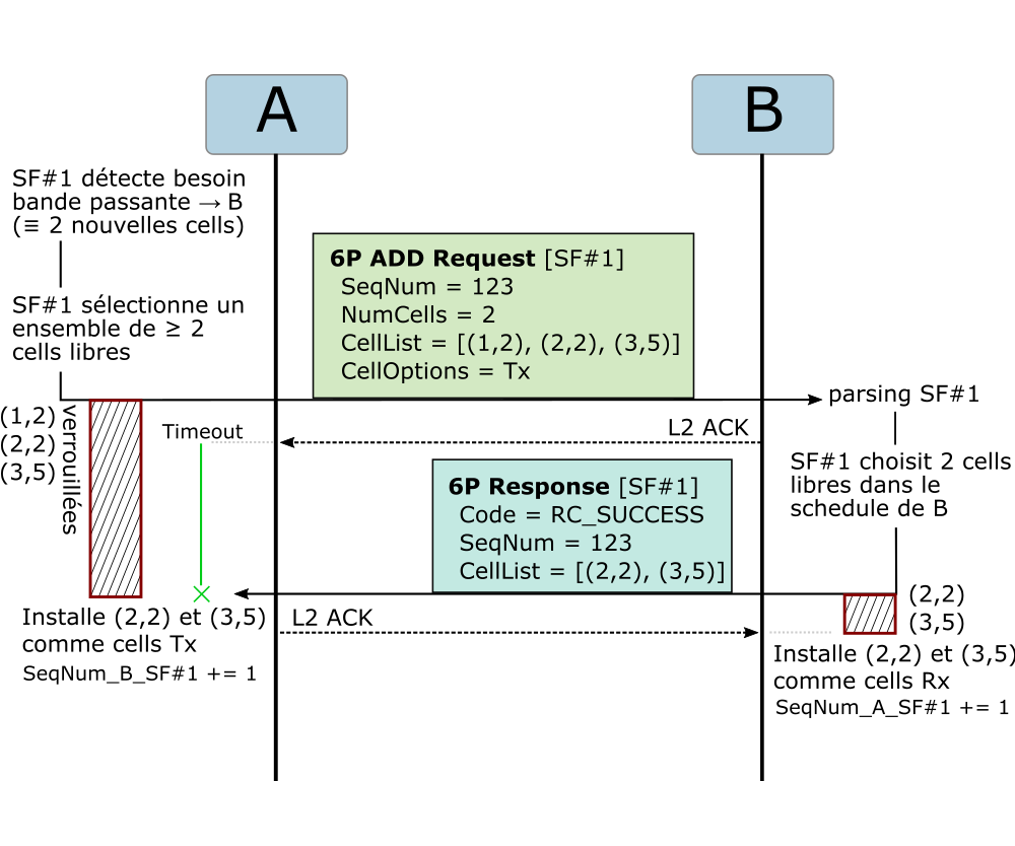
\includegraphics[width=0.99\textwidth]{6P_2-steps}
		\caption{Transaction 2-steps (commande ADD)}
		\label{fig:2-steps}
	\end{minipage}\hfill
	\begin{minipage}{0.5\textwidth}
        \centering
        \hfill
		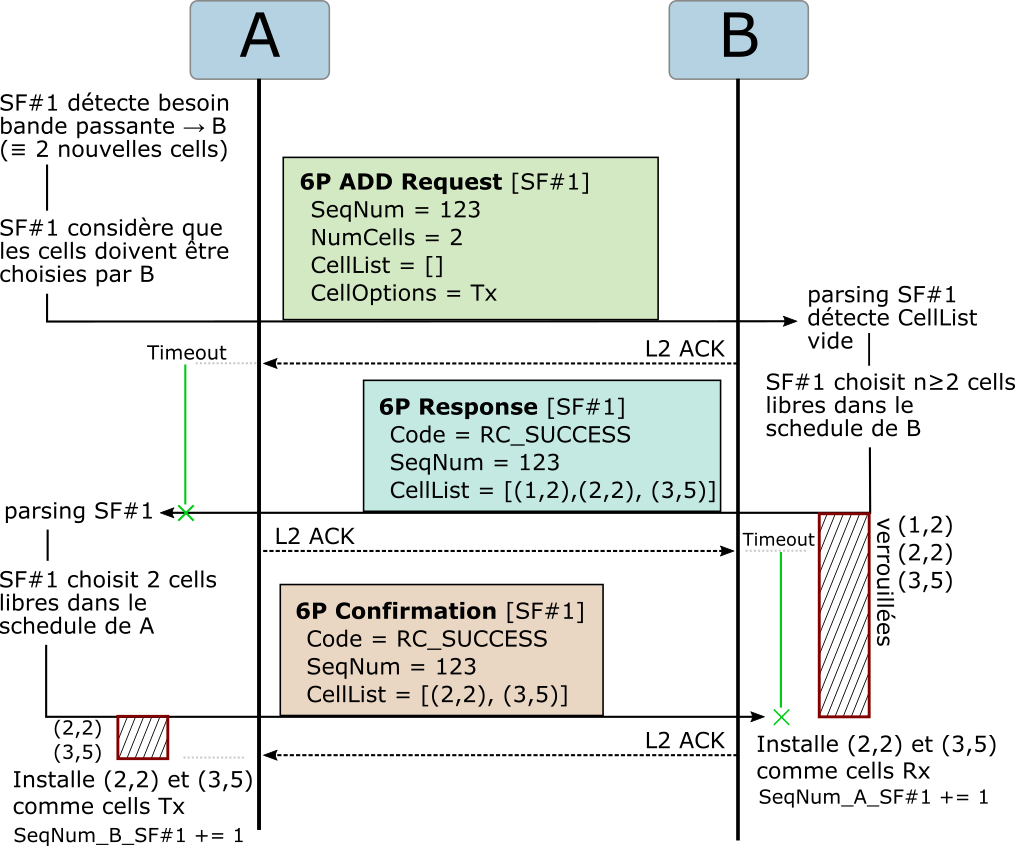
\includegraphics[width=0.99\textwidth]{6P_3-steps}
		\caption{Transaction 3-steps (commande ADD)}
		\label{fig:3-steps}
	\end{minipage}	
\end{figure}

\newpage

	\subsection{Couche d'adaptation à IPv6 - 6LoWPAN}
	\label{6LoWPAN}

\par Les WSNs se reposant sur IEEE802.15.4, et plus généralement les LLNs ont des caractéristiques qui rendent difficile l'adoption directe d'IPv6 comme couche réseau de ces réseaux. Notamment, le MTU minimal par défaut de IPv6 qui est de 1280 bytes n'est pas adapté pour une frame 802.15.4 limitée à 127 bytes. Le header IPv6 de 40 bytes réduit fortement la charge utile du paquet : considérant une frame sécurisée par 802.15.4, la frame ne transporte plus que 33 bytes de données. D'autres problématiques viennent également s'ajouter : adaptation du mécanisme de SLAAC (StateLess Address Auto-Configuration), support du broadcast dans tout le sous-réseau, donc du multihop pour atteindre les nœuds qui ne sont pas à portée directe, mécanismes de sécurité (obtention des adresses, génération d'adresses), etc \cite{rfc7554}. La couche d'adaptation 6LoWPAN met en place des mécanismes rendant possibles les communications IPv6 avec et dans un WSN. Les 3 services principaux que 6LoWPAN et ses extensions assurent sont les compressions d'headers, la fragmentation de paquet et l'auto-configuration d'adresse.\\

Pour offrir une couche d'adaptation générique pouvant utiliser un service indépendamment de l'autre, 6LoWPAN définit des sous-headers de différents types :
\vspace{0.2cm}

\begin{enumerate}
\item \textit{No 6LoWPAN} : le paquet contenu n'est pas compatible avec les mécanismes de 6LoWPAN
\vspace{0.1cm}
\item \textit{Mesh Addressing Header} : permet le forwarding des frames à la couche lien, et donc le multihop géré à la couche d'adaptation
\vspace{0.1cm}
\item \textit{Dispatch Header} : compression de headers ciblés par plusieurs schémas (IPv6, UDP, RPL, etc.)
\vspace{0.1cm}
\item \textit{Fragmentation Header} : gestion de la fragmentation et du ré-assemblage du contenu du paquet  
\end{enumerate}

\subsubsection{Mesh Addressing Header : forwarding}

\par Le standard 802.15.4 ne définit aucune forme de routage et se repose donc sur les couches supérieures. On distingue deux schémas de routage impactant également la fragmentation :
\begin{enumerate}
\item \textit{mesh-under} : routage par 6LoWPAN utilisant le mesh addressing header pour maintenir les adresses \textit{originator} et \textit{destination} (short ou extended dans le PAN) des deux extrémités de la communication, les nœuds intermédiaires forwardant les fragments du paquet sur base de ces adresses. On a donc une fragmentation effectuée par le nœud originator et un ré-assemblage une fois tous les fragments arrivé au nœud destination.
\vspace{0.1cm}
\item \textit{route-over} : routage délégué à la couche IP par un protocole qui devra donc procéder au ré-assemblage du paquet à chaque nœud sur le chemin et maintenir une table de routage. Le protocole utilisé peut être RPL.
\end{enumerate}

\vspace{0.1cm}

Utiliser le mesh-under permet d'avoir un délai de transmission plus court, au détriment de la fiabilité car un fragment perdu implique une retransmission complète de tous les fragments \cite{wiki:6LoWPAN}.

\subsubsection{Dispatch header : compression d'headers}

\par Plusieurs schémas d'encodage ont été définis, ceux-ci tirent parti du fait que certaines valeurs de champs peuvent être : inférées à partir d'informations déjà contenues dans la frame, réduites à un ensemble de valeurs communes ou encore dérivée d'un contexte partagé. \textit{LOWPAN\_IPHC} est utilisé pour laisser tomber les champs IPv6 \textit{Length} et \textit{Hop-Limit} et compresser les adresses source et destination selon leur nature. Dans le meilleur des cas, c'est-à-dire considérant l'utilisation d'adresses link-local et un unique saut, le header IPv6 peut être réduit à 2 bytes. Dans une communication multihop, il peut être compressé jusqu'à 7 bytes. Le schéma \textit{LOWPAN\_NHC} gère les Next Headers IPv6 et les champs UDP tels que l'indicateur de longueur, la checksum et les ports. Dans le cas où les ports utilisés sont courants, le header UDP peut être compressé en 2 bytes. Dans le cas où le route-over est utilisé, 6LoRH \cite{rfc8138} peut être utilisé pour compresser les informations que RPL rajoute dans les paquets (par exemple l'identificateur de l'instance RPL). 

\newpage

\subsubsection{Fragmentation header : fragmentation}

\par Le header de fragmentation fait 4 ou 5 bytes et permet d'emblée de distinguer le premier fragment  des autres, celui-ci contenant donc le header IPv6 (compressé ou non). Les valeurs reprises dans le header de fragmentation sont :
\vspace{0.2cm}
\begin{itemize}
\item[$\bullet$] \textit{dispatch} : séquence de bits indiquant s'il s'agit du premier fragment
\vspace{0.1cm}
\item[$\bullet$] \textit{datagram\_size} : la taille totale du paquet avant sa fragmentation
\vspace{0.1cm}
\item[$\bullet$] \textit{datagram\_tag} : identifie de façon unique le paquet originel duquel provient le fragment
\vspace{0.1cm}
\item[$\bullet$] \textit{datagram\_offset} : la position du fragment dans le paquet (pour les fragments suivant le premier)
\end{itemize}

\vspace{0.4cm}

\par Le problème inhérent à cette façon basique de procéder est que la perte d'un fragment empêche le ré-assemblage du paquet complet, condamnant les nœuds à recommencer la transmission entière. Des mécanismes d'acquittement sélectif ont été mis en avant pour palier à cela \cite{ietf-6tisch-architecture-28} \cite{wiki:6LoWPAN}. Une fois un paquet IPv6 totalement ré-assemblé par la couche 6LoWPAN, il est transmis à la couche IP supérieure qui opère la décision de routage.

\subsubsection{L'auto-configuration des interfaces en IPv6}

\par Dans un réseau traditionnel, le mécanisme de ND (\textit{Neighbor Discovery}) peut être employé par un nœud pour assigner de façon autonome des adresses IPv6 à ses interfaces, tout en garantissant l'unicité de celles-ci. Cependant, le mécanisme de découverte fait l'hypothèse que le broadcast est effectif sur tout le domaine, ce qui n'est pas le cas pour un nœud de WSN. Des mécanismes de multicast/broadcast sont spécifiés par 6LoWPAN au travers du dispatch header \textit{Broadcast Header}. Cependant, le ND induit un trafic multicast trop important pour un WSN \cite{wiki:6LoWPAN}, incitant à une reconception du mécanisme qui standardisée par 6LoWPAN ND \cite{rfc6775}.\\

\par Pour éviter le trafic multicast généré par les messages de DAD (\textit{Duplicated Address Detection}), les nœuds enregistrent leur adresse auprès d'un routeur qui maintient en cache toutes celles utilisées dans le réseau 6LoWPAN, associée à un temps d'expiration donné. Les requêtes d'enregistrement sont routées vers le 6LBR, dans des messages ARO (\textit{Address Registration Option}) entre un nœud et un routeur (nœuds capable de router vers la racine RPL) et dans des messages ABRO (\textit{Authoritative Border Router Option}) entre ces routeurs et le 6LBR (racine RPL). 

\vspace{0.4cm}

	\begin{figure}[!h]
	\centering
	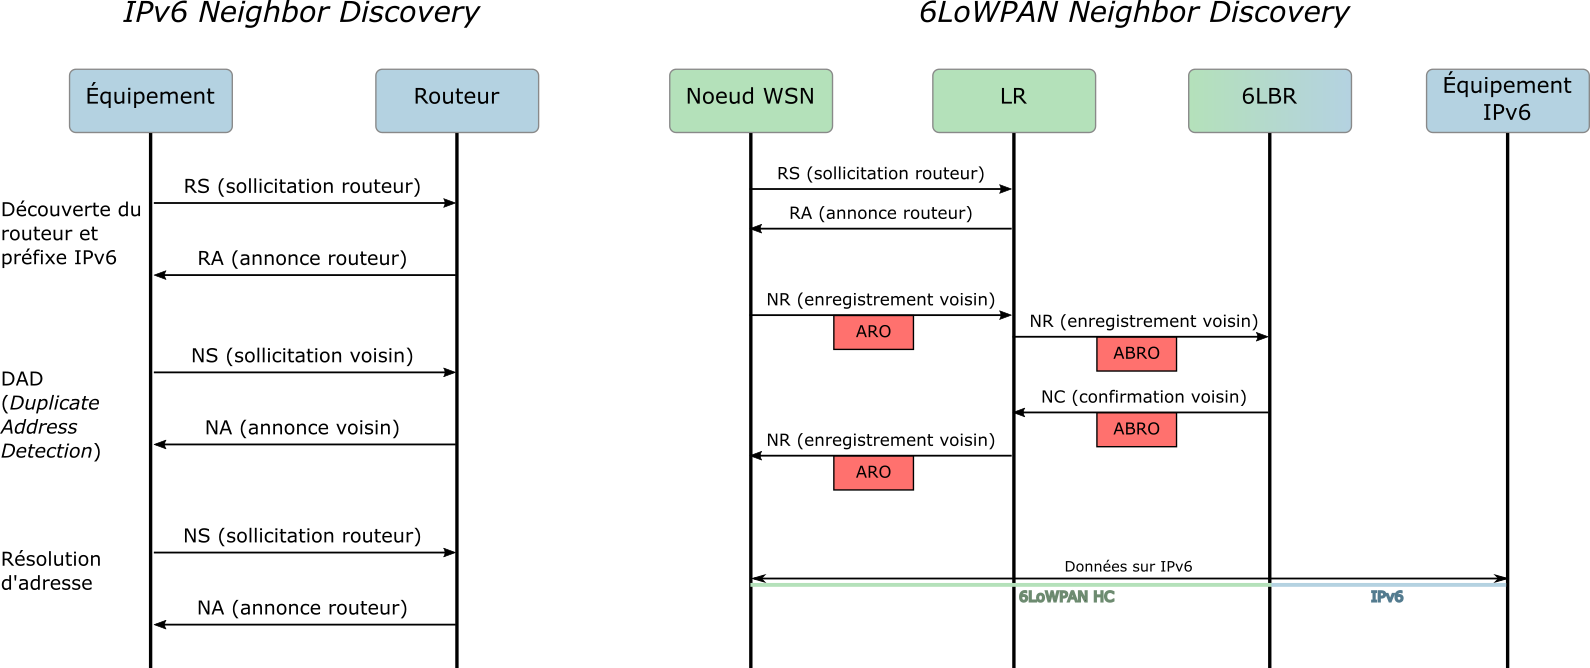
\includegraphics[width=\linewidth]{6LoWPAN-ND}
	\caption{Différences entre IPv6 ND traditionnel et 6LoWPAN ND}
	\label{fig:6LoWPAN-ND}
	\end{figure}


\newpage	
	
	\subsection{Couche réseau et routage - RPL}
	\label{RPL}
	
\par RPL (\textit{Routing Protocol for LLNs}, \cite{rfc6550}) est un protocole de routage à vecteurs de distance proactif, adapté aux communications MP2P qui sont communes dans un WSN. Typiquement, on a dans ces réseaux des communications multihops convergeant vers un point de collecte non restreint. Les topologies que RPL établit sont composées de DODAG(s) (\textit{Destination Oriented Directed Acyclic Graph}) similaires à des arbres, dont la racine est typiquement le 6LBR (voir \wordlink{Section}{archWSN}). Chaque nœud du réseau doit donc avoir au minimum un parent (excepté la racine \textit{Root}) et peut servir de parent à plusieurs autres nœuds, à condition de supporter des capacités de routage. Un nœud \textit{host} peut rejoindre le réseau en tant que feuille (\textit{leaf}) en ne supportant qu'en partie RPL, ne routant que les paquets qu'il génère lui-même. Ces topologies sont construites par les nœuds sur base de différentes métriques et attributs arbitraires, qui sont exploités par une OF (\textit{Objective Function}) pour adapter de façon optimale la topologie à des critères donnés. Des métriques classiques sont par exemple le nombre de sauts, le débit du lien, la fiabilité tandis ce que les attributs sont relatifs à l'état du nœud : sa source d'énergie, ses limitations de calcul/stockage, etc. Plusieurs applications peuvent être effectives conjointement dans un même WSN, aussi chacune est liée à une \textit{Instance} RPL s'appuyant sur un DAG (ensemble de DODAGs) et une OF.\\

\par À chaque nœud d'un DODAG est associé un rang représentant sa ``distance" avec la racine, c'est-à-dire le coût à considérer pour joindre la racine en passant par ce nœud, selon l'OF. RPL suit donc une approche ``en gradient", remonter vers la racine revenant à emprunter un chemin dont les rangs sont strictement dégressifs. Pour sélectionner un parent parmi ses voisins atteignables dans le réseau, un nœud compare leurs rangs respectifs en tenant compte du coût nécessaire pour communiquer avec chacun. L'OF définit ce qui compose ces deux éléments (quelles métriques) et le calcul à appliquer, retournant une valeur correspondant au rang potentiellement obtenu pour chaque. Le parent préféré sera alors celui qui minimise le rang retourné. Une fois associé avec, il peut continuer à évaluer ses voisins de la sorte pour adapter la topologie de façon dynamique, mais n'opérera un changement que si la différence de rang est significative (hystérèse). La \wordlink{Figure}{fig:OF} illustre la sélection d'un parent préféré $P$ parmi $P_N$ candidats, certains étant d'office éliminés car un de leur attribut ne respecte pas une contrainte préliminaire (imposée également par l'OF). L'OF est ici additive, mais peut prendre une forme arbitraire.


	\begin{figure}[!h]
	\centering
	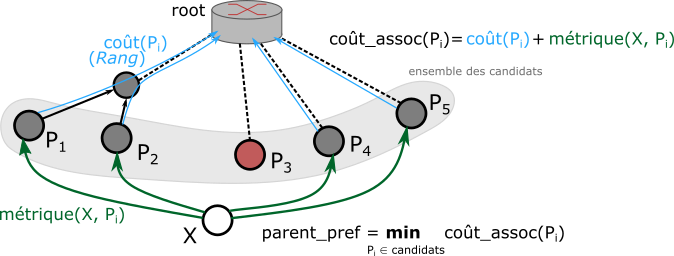
\includegraphics[width=0.85\linewidth]{OF_sel_parent}
	\caption{Sélection d'un parent préféré par un nœud X utilisant une OF arbitraire}
	\label{fig:OF}
	\end{figure}

\vspace{0.3cm}

Afin de se comparer aux autres noeuds dans la topologie, un noeud $N$ utilise l'équation suivante :
\[
DAG_{Rank(N)} = \floor{\frac{Rank(N)}{MinHopRankIncrease}}
\]

\noindent Où $Rank(N)$ est le rang que le noeud $N$ a calculé pour lui-même et $MinHopRankIncrease$ est la valeur de l'écart minimum entre deux rangs, représentant la différence minimum entre le rang d'un noeud et les rangs de ses possibles parents (spécifique à l'implémentation).

\newpage

\par Un exemple de métrique communément utilisée par une OF additive est l'ETX (\textit{Expected Transmission Count}). Elle représente le nombre moyen de (re)transmissions requises pour transmettre avec succès un paquet à un voisin (l'ETX d'un chemin multihop est l'addition des ETX de chaque saut). Sa valeur peut être estimée sur $numTx$ transmissions en considérant le nombre d'ACK reçus en retour : 
\begin{equation}
ETX = \frac{numTx}{numTxAcked} \geq 1
\end{equation}

\noindent Ces valeurs peuvent être obtenues en pratique depuis l'abstract neighbor table maintenue par la couche intermédiaire 6top \cite{ietf-6tisch-architecture-28}.


\par RPL utilise ICMPv6 pour transporter l'information utile à la construction et au maintient de la topologie, à travers plusieurs types de messages de signalement : 
\vspace{0.2cm}
\begin{itemize}
\item[$\bullet$] DIO (\textit{DODAG Information Object}) : multicast par les nœuds déjà dans la topologie (\textit{all-RPL-nodes address} \texttt{FF02::1A}) à intervalle de temps variable contrôlé par l'algorithme \textit{Trickle}. Contient la version du DODAG et l'ID de l'instance dans laquelle le nœud émetteur évolue, ainsi que son rang, les métriques, les contraintes et l'OCP (\textit{OF Code Point}) identifiant l'OF à utiliser. Un nœud souhaitant intégrer la topologie se sert de ces informations, émises par différents nœuds en faisant partie, pour sélectionner le parent qui l'y raccrochera. Un DIO permet donc d'établir des routes ascendantes.
\vspace{0.2cm}
\item[$\bullet$] DIS (\textit{DODAG Information Solicitation}) : émis en broadcast par un nœud souhaitant recevoir un DIO (évite une attente passive).
\vspace{0.2cm}
\item[$\bullet$] DAO (\textit{DODAG Advertisement Object}) : émis par un nœud vers la racine, permettant de construire des routes descendantes. Le support de ces routes peut se faire en deux modes différents : \textit{storing} et \textit{non-storing}. En mode non-storing, seule la racine maintient le nécessaire pour router vers le bas, obligeant tout paquet à remonter jusqu'à elle pour insérer dans le paquet la liste des nœuds intermédiaires. En mode storing, des nœuds intermédiaires maintiennent des tables de routage et sont donc capable de rediriger d'eux-mêmes le paquet vers le bon nœud enfant. 
\end{itemize}
 
\vspace{0.5cm}

\par La dissémination de l'information (par émission de DIOs) est régulée par l'algorithme dit du Trickle, paramétrable pour établir un compromis entre la faculté d'adaptation/expansion de la topologie et la surcharge de trafic dans le réseau. L'idée de l'algorithme est d'éviter de répandre trop de fois la même information si elle n'apporte rien, c'est-à-dire qu'elle est consistante avec l'état actuel, déjà connu. Ainsi, à la détection d'une inconsistance doit correspondre une augmentation de la fréquence d'émission de DIOs signalant le nouvel état consistant. La notion de consistance dépend du contexte, cela peut par exemple correspondre au numéro de version du DODAG courant \textit{DODAGID}, renouvelé suite à une reconstruction de la topologie. L'algorithme est paramétré par $I_{min}$ et $I_{max}$ les bornes extrémales de l'intervalle de temps entre deux transmissions et $k$ un entier qui sert de seuil de redondance à partir duquel une information ne sera pas relayée. Les variables suivantes sont utilisées : $c=0$ un compteur d'information reçue considérée comme consistante et donc redondante, $I=I_{min}$ l'intervalle courant et $t$ le timer. Le comportement est alors le suivant :

\begin{enumerate}
\item $c$ est mis à 0 et $t$ à une valeur aléatoire tirée dans $[\frac{I}{2}, I]$
\item quand une inconsistance est détectée dans la suite, $I \leftarrow I_{min}$ et retour en 1.
\item tant que $t$ n'a pas expiré, si un message consistant est reçu, $c \leftarrow c+1$
\item quand $t$ expire, si $c < k$ alors un DIO est émis
\item arrivé à la fin de l'intervalle $I$, $I \leftarrow \text{min}(2I, I_{max})$ et retour en 1.
 
\end{enumerate}

\newpage

	\subsection{Couches transport et application - CoAP sur UDP}
	\label{CoAP}
	
\subsubsection{Transport par UDP}

\par Les services que TCP assure traditionnellement dans les communications, tels que la fiabilité et le contrôle de congestion, se révèlent inappropriés dans le cadre de LLNs. Ils introduisent une surcharge trop importante de trafic dans un réseau restreint, de par le nombre de communications et les headers nécessaires. Les pertes récurrentes de paquets dans un LLN, dûes à sa nature, sont également mal interprétées par TCP qui y voit les effets d'une congestion et réagit en conséquence à tort. Des adaptations des mécanismes et allégements de TCP ont été proposés \cite{stack-IoT}, mais le fait que les deux hôtes communiquant (ou un équipement intermédiaire de traduction) doivent en supporter l'implémentation reste un frein important. De plus, cela ne correspond pas à l'idée d'interopérabilité transparente entre les réseaux restreints de l'IoT et le reste d'Internet.\\

\par UDP a donc été choisi pour assurer le transport dans la pile 6TiSCH, déléguant l'implémentation de mécanismes de contrôle à la couche applicative. UDP est léger, surchargeant peu les paquets et ne maintenant aucun état relatif aux messages envoyés. En contrepartie, il ne garantit pas de fiabilité, de mécanismes de détection de messages dupliqués et de contrôle de flux. Afin de réduire encore davantage la charge liée au transport par UDP, 6LoWPAN assure une compression efficace, réduisant les headers UDP jusqu'à seulement 2 bytes.

\subsubsection{CoAP}

CoAP (\textit{Constrained Application Protocol}, \cite{rfc7252}) apporte une réponse au besoin d'implémentation d'une adaptation de l'architecture RESTful aux LLNs. Une intégration directe du modèle client/serveur sur lequel HTTP se repose pour offrir des services Web dans Internet n'est pas envisageable. Effectivement, ce modèle fait l'hypothèse d'un transport fiable et d'une fragmentation gérée de façon transparente dans les couches plus basses. UDP ne permet pas d'assurer une fiabilité en matière de transport, et bien que 6LoWPAN gère la fragmentation, elle reste coûteuse et peut rendre le LLN inopérant \cite{stack-IoT}. CoAP définit un sous-ensemble des fonctionnalités d'une architecture RESTful, spécialisant son utilisation aux réseaux restreints. Une attention particulière est portée au maintient d'une interopérabilité maximum avec HTTP, permettant des interactions entre des équipements supportant CoAP et HTTP. CoAP se spécialise donc dans les communications M2M, se différenciant de HTTP sur plusieurs points :
\vspace{0.2cm}
\begin{itemize}
\item[$\bullet$] les équipements n'endossent pas systématiquement le même rôle de serveur/client
\vspace{0.1cm}
\item[$\bullet$] les échanges de messages sont asynchrones
\vspace{0.1cm}
\item[$\bullet$] les mécanismes de fiabilité sont implémentés au niveau applicatif par CoAP lui-même
\vspace{0.1cm}
\item[$\bullet$] la facilitation du déploiement des mécanismes de \textit{caching}/\textit{proxying}
\vspace{0.1cm}
\item[$\bullet$] minimisation de l'\textit{overhead} lié aux headers, limitation de l'utilisation d'ASCII
\end{itemize}

\vspace{0.6cm}

\par CoAP est composé de deux sous-couches logiques : la couche \textit{Message} et la couche \textit{Request/Response}. La couche Message est la première au dessus de UDP, apportant le contrôle des communications nécessaire pour palier aux manquements de ce dernier. Elle considère 4 types de messages auxquels sont associés des rôles différents dans la communication asynchrone. Les mécanismes de retransmission et de détection de messages dupliqués s'appuient sur cette sous-couche et les attributs qu'elle définit. La sous-couche suivante (Request/Response) est relative à la sémantique des messages et leur contenu. Une \textit{Request}, émise par le nœud alors considéré comme client, décrit une certaine méthode appliquée à une ressource du serveur. Par exemple, une méthode \texttt{GET} ciblant une ressource désignée par un URI. Une \textit{Response} désigne le message émis en retour par le serveur, contenant le résultat du traitement de la requête, auquel est associé un code de retour. Dans l'exemple précédent, cela peut être un message d'erreur contenant la chaine ``Not Found" accompagnée d'un code \texttt{4.04}.\\

\par Dans chaque header de message, on retrouve un champ \textit{Message ID} de 16 bits (la \wordlink{Figure}{fig:CoAP_pkt} illustre le format d'un message). Les quatre types de message transportent les Requests/Responses indépendamment de leur sémantique (la couche logique Message agissant en dessous). Le champs \textit{Type} de 2 bits dans le header indique toujours un type parmi les quatre disponibles.

\newpage

\begin{enumerate}[leftmargin=*]
\setcounter{enumi}{-1}
\item \textit{Confirmable} (CON) : message à acquitter par le serveur, qui doit répondre par un message ACK pouvant potentiellement transporter (\textit{piggybacking}) la réponse du serveur à la Request. Si la réponse à la Request n'est pas immédiatement disponible (temps d'acquisition d'une mesure par exemple), l'ACK peut être renvoyé directement, suivi par la réponse dans message CON une fois le traitement effectué (\wordlink{Figure}{fig:CoAP_CON}). Le message ID permet de faire le lien entre le message initial et son ACK, l'ACK transportant le même ID. Si aucun ACK correspondant n'est reçu, un mécanisme d'\textit{exponential backoff} gère les retransmissions.
\vspace{0.1cm}

\item  \textit{Non-Confirmable} (NON) : message ne nécessitant pas d'ACK ou de RST si son contenu n'a pas pu être traité. Cela ne signifie pas qu'à une Request envoyée dans un message NON, il n'y aura aucune Response de la part du serveur : ces deux messages ne seront juste pas acquittés et auront un Message ID différent. Dès lors, la corrélation entre ces Request et Response se fait en utilisant un mécanisme de \textit{token} (\wordlink{Figure}{fig:CoAP_NON}).
\vspace{0.1cm}

\item \textit{Acknowledgement} (ACK) : confirme la bonne réception d'un message CON à son émetteur, transportant le même Message ID. Peut potentiellement porter en même temps la Response à une Request pour limiter le trafic sur le réseau (mécanisme de piggybacking).
\vspace{0.1cm}

\item \textit{Reset} (RST) : message renvoyé par un nœud s'il n'est pas capable de traiter un message CON ou potentiellement NON (pas capable de produire un message d'erreur correspondant).
\end{enumerate}

\vspace{0.2cm}

\par La détection des messages dupliqués se fait sur base des Message IDs indiqués par les messages reçus. Étant donné que le modèle de communication est asynchrone, un mécanisme de token est employé pour corréler une Response à sa Request, deux messages présentant un même token concernant donc une ressource identique. Un token est une séquence pseudo-aléatoire de 0 à 8 bytes que chaque client devrait générer et intégrer dans chacune de ses Requests. Dans le paquet, il est placé à la suite du header CoAP de taille fixe et suivi des potentielles \textit{Options} CoAP et du Payload applicatif s'il y en a un (voir \wordlink{Figure}{fig:CoAP_pkt}). Les Options sont des conteneurs de la forme \textit{Type-Length-Value} présents dans les Requests et Responses, permettant de transporter des informations complémentaires exploitables dans le contexte à la manière des en-têtes HTTP. Par exemple, l'URI d'une ressource ciblée est divisée en plusieurs Options \texttt{Uri-Host}, \texttt{Uri-Port}, etc. Le champs \textit{Code} (8 bits) est divisé en une classe \textit{c} (3 bits) et un détail \textit{dd} (5 bits), définissant une correspondance directe avec les codes HTTP. Par exemple, $c$=\texttt{0} pour une Request permet d'indiquer une commande \texttt{GET, POST}, etc. en fonction de $dd$, $c=4$ pour une Response indique une erreur client ($dd$=\texttt{04} donne \texttt{4.04}, erreur ``\texttt{Not found}").


\begin{figure}[!ht]
	\centering
	\begin{minipage}{0.39\textwidth}
		\centering
		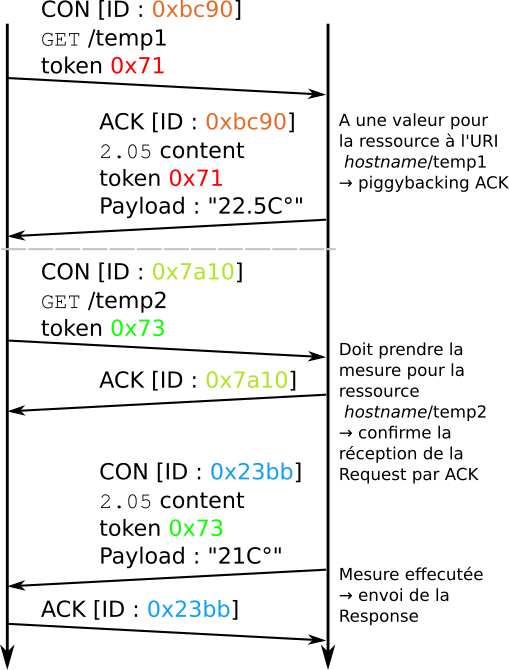
\includegraphics[width=\textwidth]{CoAP_messaging_CON}
		\caption{Message CON et piggybacking de la Response dans l'ACK}
		\label{fig:CoAP_CON}
	\end{minipage}\hfill
	\begin{minipage}{0.59\textwidth}
        \centering
        
		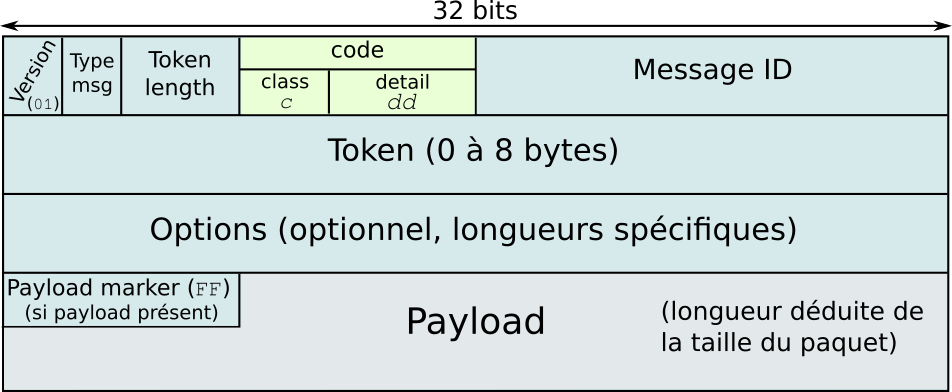
\includegraphics[width=0.85\linewidth]{CoAP_pkt}
		\caption{Format d'un message CoAP \cite{rfc7252}}
		\label{fig:CoAP_pkt}
		\vspace{0.1cm}
		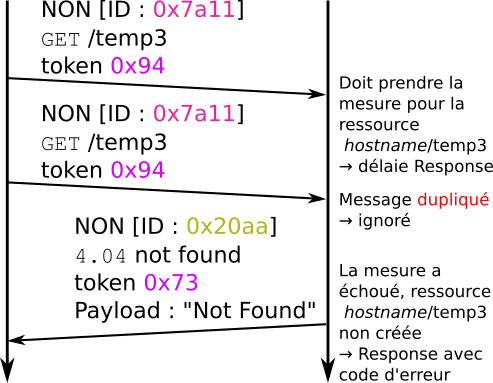
\includegraphics[width=0.59\textwidth]{CoAP_messaging_NON}
		\caption{Message NON et détection de duplicata}
		\label{fig:CoAP_NON}
		
		
	\end{minipage}	
\end{figure}



\newpage

CoAP utilise un schéma d'URI similaire à HTTP, identifiant la ressource sur un serveur dit \textit{origin server} par un chemin pointant vers l'élément dans sa structure hiérarchique. L'origin server est identifié soit par un nom d'hôte à résoudre par un mécanisme similaire au DNS, soit par une adresse IP (CoAP supporte IPv4 et IPv6). Un serveur écoute sur un port UDP spécifié dans l'URI,  ou le port 5683 par défaut. Une requête est paramétrable avec un nombre arbitraire d'arguments terminant l'URI. Tout comme HTTP avec son homologue HTTPS, CoAP supporte la sécurisation au niveau du transport par DTLS. Le schéma d'URI est alors différent (\texttt{coaps} et non \texttt{coap}), mais ne sera pas considéré ici. Le schéma est le suivant \cite{rfc7252} :
\vspace{0.1cm}
\begin{center}
\texttt{coap-URI} = ``coap:" ``//" \textit{hostname} [``:" \textit{port}] \textit{path-abempty} [``?" \textit{query}] 
\end{center}

\par Où \textit{hostname} permet d'identifier le serveur, \textit{path-abempty} est le chemin absolu de la ressource sur le serveur (peut être vide sous certaines conditions) et \textit{query} est une chaîne paramétrisant la requête avec des arguments de la forme \textit{key}=\textit{value} séparés par ``\&". Un URI à transporter dans un message est fragmenté sous la forme d'Options \texttt{Uri-Host}, \texttt{Uri-Port}, \texttt{Uri-Path} et \texttt{Uri-Query} (ensemble désigné par le terme \textit{Uri-*}). Les deux dernières peuvent être multiples, une Option \texttt{Uri-Path} correspondant à un segment du chemin (chaîne entre deux ``/") et une Option \texttt{Uri-Query} correspond à une paire (\textit{key}, \textit{value}). Une implémentation de CoAP doit supporter la découverte de serveur/service et de ressource dans le cadre de communications M2M. Cela est géré d'une part part un support de l'adresse multicast \texttt{all-CoAP-node} (\texttt{FF0\textit{X}::FD}) et d'autre part en définissant un point d'entrée pour l'accès aux ressources, par défaut à l'URI \texttt{/.well-known/core}. Ce dernier permet de décrire les ressources disponibles sur le serveur.\\

\vspace{0.4cm}

\par Le mécanisme de \textit{caching} permet de diminuer le trafic sur le réseau et de réduire les délais de réponse. CoAP se repose dessus pour optimiser les communications, permettant à un nœud intermédiaire entre le client et le serveur de réutiliser une Response antérieure stockée pour répondre à une Request ciblant la même ressource. À la différence d'HTTP, CoAP définit un message comme \textit{cachable} selon le code de la Response, celle-ci étant accompagnée d'une Option \textit{Max-Age} indiquant le temps de validité de l'information stockée le cas échéant.\\

\par Un proxy est un \textit{CoAP endpoint} (supportant les services du protocole CoAP) qui peut être délégué par un client pour effectuer des Requests ``à sa place". Il peut également faire du caching. Il apporte une augmentation des performances du réseau, permet d'accéder aux ressources protégées d'un serveur ou délayer la Request si le nœud serveur est endormi et ne peut répondre. Il peut faire la traduction entre CoAP et d'autres protocoles applicatifs, HTTP notamment. Les Requests vers un proxy peuvent indifféremment être des messages CON et NON. La spécification \cite{rfc7252} distingue deux types de proxy :
\vspace{0.2cm}
\begin{itemize}
\item[$\bullet$] \textit{forward-proxy} : ce proxy est explicitement désigné par le client qui passe l'URI de la ressource ciblée en conscience de cause dans des Options significatives pour le proxy. Soit sous la forme d'une chaîne contenant l'URI complet dans l'Option \textit{Proxy-Uri}, soit en fournissant l'Option \textit{Proxy-Scheme} indiquant le schéma cible (\texttt{coap}, \texttt{http}, ...) et les Options Uri-*. Ces Options vont alors être consommées par le proxy pour relayer la Request vers l'origin server qu'elles indiquent, supplantées par les Options Uri-* telles que celles qu'un client utiliserait pour une Request directe vers l'origin server (rôle alors de fait endossé par le proxy). Cela implique un parsing de l'URI et la fragmentation en Options Uri-* dans le cas de l'usage de l'Option Proxy-Uri et la suppression de l'Option Proxy-Scheme dans le second cas. Le proxy effectue la traduction vers le protocole indiqué par le schéma dans l'URI ou l'Option Proxy-Scheme.
\vspace{0.2cm}
\item[$\bullet$] \textit{reverse-proxy} : ce proxy est renseigné comme l'origin server dans l'URI que le client intègre dans sa Request, construite en considérant le proxy comme jouant directement le rôle du serveur. Le proxy agit alors de manière arbitraire, le comportement résultant se base sur le contenu de la Request et la configuration du proxy. Vraisemblablement, il va rediriger la requête vers un serveur qu'il sait en possession de la ressource, agissant lui-même comme un client en utilisant le protocole qu'il juge adapté pour communiquer avec ce serveur.
\end{itemize}
 
\newpage

\par Un proxy qui fait de la traduction de requêtes entre protocoles (CoAP $\leftrightarrow$ HTTP notamment) est désigné par le terme \textit{cross-proxy} dans la spécification \cite{rfc7252}. CoAP supporte un sous-ensemble des fonctionnalités de HTTP, mais la correspondance entre les deux peut être faite dans les deux sens par un cross-proxy. Ainsi, on a en fonction du sens de la requête :
\vspace{0.2cm}
\begin{itemize}
\item[$\bullet$] le cross-proxy CoAP-HTTP qui permet à un client CoAP n'implémentant pas HTTP d'accéder à une ressource détenue par un serveur HTTP. En fonction du type de proxy, le client CoAP construit sa requête différemment :
	\begin{itemize}
	\item[$\triangleright$] vers un forward-proxy, soit en intégrant l'URI commençant par le schéma \texttt{http:...} dans l'Option Proxy-Uri, soit en instanciant les Options Uri-* accompagnées de l'Option Proxy-Scheme renseignant la valeur ``http"
	\item[$\triangleright$] vers un reverse-proxy, en lui adressant une Request comme si c'était le serveur à contacter, que le proxy devra traiter de manière à répondre comme s'il était le serveur	
	\end{itemize}	 
\vspace{0.1cm}
\item[$\bullet$] le cross-proxy HTTP-CoAP permet à un client HTTP de contacter un serveur CoAP, construisant sa requête en fonction du proxy considéré :
	\begin{itemize}
	\item[$\triangleright$] vers un forward-proxy, en introduisant un header HTTP \textit{Request-Line} avec la valeur associée ``coap"
	\item[$\triangleright$] vers un reverse-proxy, en forgeant sa requête comme s'il s'adressait à un serveur HTTP, que le proxy devra traiter de manière à répondre comme s'il était le serveur
	\end{itemize}	 

\end{itemize}

\par Dans le premier cas, la traduction peut être effectuée assez facilement étant donné que CoAP ne définit pas de fonctionnalités qui n'ont pas leur équivalent pour HTTP. En revanche, le second cas peut poser problème et le proxy l'implémentant devra définir des mécanismes de filtrage pour ce qui n'a pas de correspondance dans CoAP (méthodes HTTP, options et codes).

\subsubsection{CoJP et OSCORE}
\label{intro_CoJP}

\par Le protocole CoJP (\textit{Constrained Join Protocol}, \cite{ietf-6tisch-minimal-security-15}) a été élaboré par le groupe 6TiSCH pour gérer la phase sensible qu'est le raccord d'un nouveau nœud au WSN. Il fait partie d'un framework minimal \cite{ietf-6tisch-minimal-security-15} écrit pour organiser l'échange de messages nécessaire au raccord utilisant un ``canal sécurisé", tout en limitant au maximum le nombre de messages échangés. CoJP définit la sémantique des messages, encodés par des structures de données CBOR (\textit{Concise Binary Object Representation}, \cite{rfc7049}) qui seront transportées comme des payloads de messages CoAP (voir \wordlink{Figure}{fig:CoJP_stack}). Les Responses et Requests ainsi échangées sont protégées par OSCORE (\textit{Object Security for Contrained RESTful Environments}, \cite{rfc8613}) qui, en établissant un canal sécurisé, permet :
\vspace{0.1cm}
\begin{itemize}
\item[$\bullet$] une confidentialité des transmissions point à point
\item[$\bullet$] l'authentification et la garantie d'intégrité des données
\item[$\bullet$] une protection contre les attaques de \textit{replay}
\item[$\bullet$] une corrélation sécurisée entre Request et Response se correspondant
\end{itemize}

\vspace{0.2cm}

\par Les éléments liés à la couche logique Message de CoAP ne sont pas chiffrés par OSCORE car ceux-ci doivent être visible par les équipements intermédiaires, notamment les proxys. Le \wordlink{Chapitre}{joining_analysis} analyse en détail CoJP et tous les mécanismes de la pile 6TiSCH relatifs à la procédure de raccord d'un nouveau nœud au WSN.  

\vspace{0.02cm}

	\begin{figure}[!hb]
	\centering
	\includegraphics[width=0.45\linewidth]{CoJP_stack}
	\caption{CoJP et OSCORE positionnés par rapport aux couches logiques CoAP}
	\label{fig:CoJP_stack}
	\end{figure}

\newpage

\section{Principes inhérents au déploiement de la pile}
	\subsection{Synchronisation temporelle}
	\label{synchrotemp}

	Dans un réseau TDMA, les nœuds doivent restés synchronisés temporellement pour assurer les communications, ce qui revient dans le cas de TSCH à faire en sorte que tous les timeslots soient alignés et commencent au même instant pour chaque nœud. Le phénomène de clock drifting décalant les horloges des nœuds relativement les une aux autres, il est quantifié en \textit{ppm} (\textit{parts per million}). Si deux nœuds on leur horloges dérivant de façon opposée à 10 \textit{ppm} (l'une ``ralentissant" et l'autre ``accélérant"), une seconde après qu'elles aient été synchronisées elles présenteront un décalage relatif de 20 $\mu s$. Pour absorber ce décalage, la \wordlink{Section}{templatetimeslot} présentait l'usage d'une période tampon de \textit{macTsRxWait} $\mu s$ désignée par \textit{guardtime} dans la littérature. Plusieurs méthodes sont utilisées pour resynchroniser les nœuds entre eux, \cite{openWSN} exprime la durée maximum entre les resynchronisations par la formule suivante :
\vspace{-0.2cm}
\begin{align}
\text{\textit{MaxResyncPeriod}} = \frac{guardtime}{clockdrift}
\end{align}

\par Passé ce délai, les nœuds seront désynchronisés et ne pourront plus s'entendre l'un l'autre, ce qui potentiellement exclut un nœud du réseau qu'il devra rejoindre à nouveau. Typiquement, on observe un clockdrift de 10 \textit{ppm}, en se plaçant de le pire cas où il a lieu de façon opposée pour deux nœuds et considérant un guardtime de 1 ms, on a
\vspace{-0.2cm}
\begin{align*}
\text{\textit{MaxResyncPeriod}} = \frac{1 \: ms}{20 \times 10^{-6}} = 0,5 \times 10^5 \: ms = 50 \: s
\end{align*}
 
\vspace{0.2cm}
\subsubsection{Resynchronisation entre nœuds voisins} 
 
\par La resynchronisation peut se faire de façon implicite en utilisant les échanges de messages qui font partie du trafic régulier dans le WSN (paquets de données et ACKs). S'il n'y a aucun trafic (nœud endormi), un message \textit{keepalive} expressément destiné à la resynchronisation doit être échangé dans un délai inférieur à la valeur de \textit{MaxResyncPeriod} s'appliquant aux nœuds. De façon approximative, \cite{openWSN} estime le duty cycle engrangé par ces messages de maintient à $0,02\%$ (cette valeur augmentant linéairement avec le clockdrift de l'horloge). Dans une communication entre voisins, le standard IEEE802.15.4e \cite{IEEE802.15.4} considère deux méthodes pour resynchroniser les nœuds (supposant qu'un des deux est la time source de l'autre). Dans les deux cas, le receveur de la transmission calcule la différence de temps $\Delta$ entre l'instant attendu d'arrivée de la frame (fixe par rapport au début du timeslot) et le moment ou le premier symbole de la frame est réellement reçu.

\vspace{0.2cm}

\begin{itemize}
\item[$\bullet$] \textit{ACK-based} : permet à l'émetteur de resynchroniser son horloge sur celle du receveur
\begin{enumerate}
\item L'émetteur envoie le premier symbole de la frame \textit{macTsTxOffset} $\mu s$ après le début du timeslot selon son horloge, ce qui devrait se produire \textit{macTsRxOffset} $+ \frac{\text{\textit{guardtime}}}{2} \: \mu s $ après le début du timeslot selon la perception du temps du receveur si les deux horloges étaient parfaitement synchronisées 

\item Le receveur marque le \textit{timestamp} du moment où le premier symbole est reçu et calcule la correction $\Delta = \textit{macTsRxOffset} + \frac{\textit{guardtime}}{2} - \textit{timestamp} \: \mu s$. On a alors $\Delta < 0$ si le receveur est ``en retard" par rapport à l'émetteur en terme de perception du temps (et vice-versa si $\Delta > 0$).

\item Le receveur renseigne cette valeur de $\Delta$ dans l'IE \textit{Time Correction} de la frame ACK qu'il renvoie à l'émetteur (à la suite dans le même timeslot).

\item L'émetteur reçoit l'ACK et, si le receveur est renseigné comme sa time source, se resynchronise dessus en ajustant son horloge de $\Delta \: \mu s$ (valeur signée).
\end{enumerate}

\vspace{0.2cm}

\item[$\bullet$] \textit{Frame-based} : permet au receveur de resynchroniser son horloge sur celle de l'émetteur
\begin{enumerate}
\item Déroulement identiques aux étapes 1 $\rightarrow$ 2 de la méthode ACK-based.
\item Si le receveur a l'émetteur renseigné comme sa time source, se resynchronise dessus en ajustant son horloge de $\Delta \: \mu s$ (valeur signée), un ACK est renvoyé mais il ne servira pas à la resynchronisation.
\end{enumerate}

\end{itemize}

\newpage

\subsubsection{Synchronisation globale du réseau}

\par La notion de temps globale, commune à tous les nœuds d'un même réseau 6TiSCH, est apportée par l'ASN. Celui-ci a été initialisé à 0 à la création du réseau et est incrémenté d'une unité à chaque timeslot expiré, ce qui implique que la durée d'un timeslot est fixe pour tous les nœuds du réseau. Encodé sur 5 bytes, considérant des timeslots de 10 \textit{ms}, ce compteur est suffisant pour une utilisation sur plus d'une centaine d'années \cite{stack-IoT}. Il est annoncé explicitement dans les EBs émis par les nœuds déjà membre du réseau (voir \wordlink{Section}{joinphase}), mais est toujours implicite dans les communications internes. Un nœud qui a une mauvaise valeur d'ASN calcule des sauts de fréquences erronés et perd toute connectivité avec les autres nœuds. Outre les calculs de fréquence, l'ASN est utilisé dans la composition du nonce pour les opérations de sécurité, de par sa nature de compteur différent à chaque communication successive dans le temps.\\

\par À n'importe quel moment, un nœud membre du réseau doit avoir un parent time source sur lequel il réajuste son horloge par les procédés ACK/frame-based. Les boucles de synchronisation temporelle doivent être évitée, aussi les relations entre time sources doivent être structurées. \cite{ietf-6tisch-minimal-security-15} soutient le fait que cette structure devrait profiter de la topologie déjà formée par RPL (DODAG), un parent time source d'un nœud étant choisi comme le parent RPL dans le DODAG. La spécification \cite{ietf-6tisch-architecture-28} va plus loin en recommandant une Instance RPL globale dédiée à la synchronisation : la TSGI (\textit{Time Synchronization Global Instance}). La configuration dépend alors de l'architecture et de la présence d'une source temporelle commune entre plusieurs WSN. Un nœud, quand il annonce le réseau avec des EBs, communique une valeur \textit{Join Priority} qui indique à quel point il serait un bon point de raccord au réseau pour un nouveau nœud. Si un nœud n'est pas encore dans le DAG associé à la TSGI, il annonce une Join Priority de \texttt{0xFF} indiquant qu'il ne peut pas être time source et ne souhaite pas servir de point de raccord. Une fois inclus à la TSGI, il annonce une Joint Priority basée sur son rang dans le DODAG qu'il a rejoint. Une faible valeur indiquant un meilleur point de raccord, cela est cohérent avec l'approche en gradient de RPL : au plus il est proche de la source temporelle du DODAG au mieux c'est.\\

\par Différentes politiques existent pour contrôler le ``trafic de resynchronisation" dans le réseau, l'objectif étant de devoir émettre un minimum de messages keepalives qui n'ont que cette utilité. D'autres trafics de contrôle réguliers peuvent conjointement servir d'appoint pour la synchronisation, notamment les messages de signalement RPL et l'émission d'EBs. \cite{ietf-6tisch-architecture-28} propose que la couche 6top puisse influer sur le timer Trickle de RPL afin de réguler l'envoi de messages de signalement DIO à une cadence qui permette aussi d'assurer le maintient de la synchronisation en parallèle. Il n'y a pas de standardisation claire de ces politiques.

\newpage

	\subsection{Formation du réseau}
	\label{joinphase}
	
Un réseau 6TiSCH se forme progressivement à partir du 6LBR auquel les nœuds restreints à portée se raccordent. Les autres nœuds qui ne sont pas à portée directe utiliseront des nœuds déjà raccordés comme intermédiaires, formant un réseau multihop. Le processus de raccord, désigné dans ce document par \textit{joining phase} est composé de deux étapes distinctes : 
\vspace{0.1cm}
\begin{enumerate}
\item L'étape de \textit{scanning/advertising} : un nœud désireux de rejoindre un réseau, appelé \textit{pledge}, écoute dans un des canaux possibles afin d'intercepter un EB émis par un nœud déjà membre du réseau. Cet EB contient toutes les informations nécessaires au pledge pour procéder au raccord en passant à l'étape suivante (synchronisation temporelle, cells à utiliser pour le reste du join, etc.).   
\vspace{0.1cm}
\item L'étape d'intégration au réseau : CoJP est utilisé par le pledge pour communiquer avec l'autorité du réseau qui validera son raccord en lui renvoyant les paramètres nécessaires à son intégration complète (notamment les clés actives dans le réseau au niveau lien ). Cet échange se fait en utilisant un nœud déjà raccordé comme intermédiaire et n'est composé que d'un message de requête et sa réponse par l'autorité. Le WG 6TiSCH en définit le format des messages et le déroulement intégral dans la spécification \cite{ietf-6tisch-minimal-security-15}.
\end{enumerate}

\vspace{0.5cm}

\par Le WG 6TiSCH envisage deux types de déploiement en fonction de la façon dont les paramètres pour procéder à l'intégration sont injectés dans les nœuds, avant qu'ils ne rejoignent le réseau. Leur application dépend directement des besoins pratiques liés au déploiement. Ces deux options sont \cite{6TiSCH-industrial-perf} :

\begin{itemize}
\item[$\bullet$] le mécanisme \textit{One-Touch} : le pledge est supposé partager une clé unique avec l'autorité du réseau sans qu'ils n'aient pour autant communiqué : elle doit leur être fournie manuellement par un moyen quelconque.
\item[$\bullet$] le mécanisme \textit{Zero-Touch} : la configuration a lieu en usine durant la fabrication de l'équipement. Le fabricant inclut un certificat digital et maintient un service de validation en ligne que l'autorité du réseau 6TiSCH pourra contacter afin de valider un certificat présenté par un pledge.
\end{itemize}

\vspace{0.1cm}

\noindent Dans le cadre de ce travail, seul le mécanisme de One-Touch est considéré car c'est celui qui permet d'avoir le plus d'emprise sur la phase de déploiement. La phase de joining One-Touch et son aspect sécurité sont étudiés dans le \wordlink{Chapitre}{joining_analysis}.\\

\par Spécifiquement conçu pour 6TiSCH, le protocole CoJP a été pensé de façon à limiter au maximum les ressources consommées par les équipements durant l'étape d'intégration, du point de vue du pledge mais également du réseau en place. En revanche, l'étape de scanning/advertising est beaucoup plus délicate, des deux côtés. Le standard IEEE802.15.4 \cite{IEEE802.15.4} ne définit ni le contenu des EBs, ni la stratégie d'émission à adopter pour les annoncer aux pledges. Les caractéristiques du contenu d'un EB (voir \wordlink{Section}{EBs}), ainsi qu'une \textit{minimal slotframe} utilisable pour leur émission sont décrits dans la spécification \cite{rfc8180}. La procédure de scanning pour capter un EB est très coûteuse pour un pledge \cite{join-TSCH-RPL}, celui-ci n'ayant à priori aucune connaissance des moments auxquels ils sont émis par les membres du réseau et dans quel canal physique.\\

\par Les principaux travaux qui s'y intéressent dans la littérature ciblent la stratégie d'annonce des EBs, permettant par des techniques variées d'ajuster le compromis temps de raccord au réseau/énergie consommée. \cite{join-TSCH-RPL} étudie l'utilisation du timer Trickle de RPL pour coupler les émissions d'EBs à celles des DIOs, les désavantages de cette technique employée en pratique dans ContikiOS, et en proposent finalement un dérivé. \cite{broadcast-strategies} considère la minimal slotframe (donc statique) qui induit un comportement similaire à slotted ALOHA, mais évite les collisions avec une approche probabiliste pour l'émission d'EB dans ces cells. \cite{ATP} étudie la possibilité d'émettre plus qu'un seul EB dans un même timeslot d'annonce, mais à des fréquences différentes pour accélérer le processus de scanning par le pledge.


\newpage

	\subsection{Ordonnancement des transmissions - \textit{minimal scheduling} avec MSF}
	\label{scheduling}

    Le WG 6TiSCH a défini une SF basique mais polyvalente, en adéquation avec la configuration minimum qui a été décrite dans la spécification \cite{ietf-6tisch-minimal-security-15}. La MSF (\textit{Minimum Scheduling Function}) fait l'objet d'un draft \cite{ietf-6tisch-msf-10} décrivant son comportement et ses interactions avec la couche 6top. Elle gère d'une part l'établissement d'un schedule minimal utilisable pour la phase de join et d'autre part l'adaptation dynamique de cells négociées entre un nœud et son parent RPL. La MSF est prévue pour un trafic régulier vers la racine. Elle utilise la minimal cell décrite dans \cite{ietf-6tisch-minimal-security-15} pour les émission broadcast d'EBs et de DIOs, distinguant trois slotframes :
    
\begin{enumerate}
\setcounter{enumi}{-1}
\item réservée au trafic de \textit{bootstrapping}, minimal cell en broadcast permettant de lancer la procédure de join
\item cells autonomes installées automatiquement pour établir une première communication directe
\item cells additionnelles négociées par le biais de transactions 6P en fonction du trafic observé
\end{enumerate}

\vspace{0.4cm}

\par MSF ne considère des communications bidirectionnelles qu'avec un nœud \textit{preferred parent}, qui n'est autre que le parent RPL une fois la topologie rejointe (ou le nœud servant d'intermédiaire lors du join). Afin de minimiser les transactions 6P, surtout si elles doivent passer par la minimal cell, MSF prévoit l'installation d'\textit{autonomous cells} dont les coordonnées sont obtenues à partir d'un hash de l'EUI-64 (extension de l'adresse MAC). Ainsi, chaque nœud est censé maintenir une cell \textit{AutoRxCell} dans la slotframe 1 dont les coordonnées (\textit{slotOffset}, \textit{channelOffset}) sont calculées à partir de l'EUI-64 de sa propre adresse (donc fixes). Le calcul tient compte du fait que la minimal cell est installée d'office et ne retourne donc jamais un \textit{slotOffset} égal à 0. Pour envoyer une frame vers un voisin, il peut de façon similaire installer une cell \textit{AutoTxCell} à partir de l'EUI-64 de ce voisin, ce dernier ayant alors déjà installé aux même coordonnées son \textit{AutoRxCell}.\\

\par La MSF gère la façon dont les communications pour le processus de join s'organisent en terme de cells, principalement en installant temporairement des cells autonomes pour le 6LoWPAN ND et l'échange CoJP, ainsi que la minimal cell pour recevoir les DIOs par la suite. Une fois la topologie intégrée (rang RPL acquis), le nœud pourra négocier ses premières cells avec son parent (slotframe 2) et annoncer des EBs et DIOs (slotframe 0). À terme de la phase de join, le nœud sera synchronisé et authentifié dans le réseau, participera à la topologie activement (selon ses capacité de routage) et possédera des cells Tx négociées vers/depuis son parent.\\

\par La négociation de cells dans la slotframe 2 a lieu en réaction à trois événements :
\begin{itemize}
\item[$\bullet$] les ressources allouées au trafic (bande passante en terme de nombre de cells) ne correspondent pas au trafic observé. Si elles sont trop faibles, la MSF déclenche une transaction \texttt{ADD} pour ajouter des cells, si les cells déjà installées sont trop peu utilisées elle déclenche une transaction \texttt{DELETE}. 
\vspace{0.1cm}
\item[$\bullet$] suite à un changement de parent dans la topologie. La MSF tente de réinstaller un nombre équivalent de cells avec le nouveau parent (transactions \texttt{ADD}), puis lance une transaction \texttt{CLEAR} avec l'ancien parent pour éliminer les cells précédemment négociées.
\vspace{0.1cm}
\item[$\bullet$] pour traiter la détection d'une collision entre schedules, suite à l'observation d'une différence de PDR (\textit{Packet Delivery Ratio} = $\frac{numTxAck}{numTx}$) entre deux cells négociées avec le parent. Cela peut arriver car la négociation est par nature un processus distribué. La MSF déclenche alors une transaction \texttt{RELOCATE} pour déplacer ces cells problématiques et les installer à des coordonnées qui n'induisent aucune collision.
\end{itemize}

\vspace{0.4cm}

\par Le draft MSF \cite{ietf-6tisch-msf-10} définit encore d'autres mécanismes, tels que le maintient intelligent d'un \textit{cell pool} dans lequel piocher les cells à ajouter ainsi que la gestion du timeout et des erreurs 6P.\\

Il existe d'autres SFs proposées, assurant des propriétés et garanties différentes en fonction des besoins intrinsèques au déploiement. On peut notamment citer le draft de la SF0 \cite{ietf-6tisch-6top-sf0-05}, LLSF pour \textit{Low Latency SF} \cite{LLSF} qui améliore SF0 en agençant les timeslots en \textit{daisy chain} et ReSF pour \textit{Recurrent Low-Latency SF} \cite{ReSF} qui utilise un modèle pour optimiser le scheduling en présence de trafic récurrent.

	
\chapter{Analyse détaillée de la sécurité pour la phase de join}
\label{joining_analysis}
\newpage

\section{Ressources et standards utilisés}

\subsection{CBOR et COSE}

CBOR (\textit{Concise Binary Object Representation} \cite{rfc7049}) est un format de données spécialement conçu pour le traitement de messages par des systèmes restreints. Le code requis pour l'encodeur et le décodeur est minimal, les messages sont de taille réduite tout en permettant l'extensibilité. La spécification se base principalement sur celles définissant le format JSON, adaptant les besoins à ceux de communications entre systèmes restreints. Les données au niveau applicatif échangées lors de la phase de join sont formatées en utilisant CBOR.\\

COSE (\textit{CBOR Object Signing and Encryption} \cite{rfc8152}) est une spécification définissant les services de sécurité associables au format CBOR. Elle décrit comment créer et traiter les signatures, les codes d'authentification de message (MAC) et le chiffrement des données sérialisées avec CBOR. Le transport de clés assisté par CBOR y est également discuté.

\subsection{OSCORE}

\subsubsection{Principes fondamentaux d'OSCORE}

OSCORE \cite{rfc8613} et sa place dans la pile 6TiSCH sont brièvement introduits par la \wordlink{Section}{intro_CoJP}. OSCORE décrit les mécanismes et concepts nécessaires à l'établissement d'un canal sécurisé au niveau applicatif entre deux nœuds comprenant CoAP, mais qui souhaitent protéger un maximum d'informations dans les messages échangés. Effectivement, certains champs CoAP (des Options notamment) doivent rester visibles par les proxys opérant comme intermédiaire au niveau applicatif entre les deux nœuds. D'autres, tels que le payload et le code du message doivent être protégés des proxys, qui pourraient sinon les consulter et les manipuler. En d'autres termes, OSCORE agit uniquement sur la couche logique Request/Response de CoAP, du client au serveur et vice-versa. Techniquement, la sécurité du canal entre ces deux points est assurée par COSE qui opère le chiffrement et les vérifications d'intégrité des champs à protéger, la protection contre les attaques replay et la liaison entre Request et Response.\\

\par L'emploi d'OSCORE dans le cadre de la phase de join est justifié par le fait qu'un pledge utilise un proxy pour échanger avec le réseau tout du long de la phase de join. Plus précisément, afin d'obtenir les informations nécessaires à son intégration dans un réseau 6TiSCH (les clés actuellement en usage notamment), le pledge va se servir du noeud déjà intégré au réseau comme d'un proxy intermédiaire (CoAP). Ce proxy va accepter les frames émanant du pledge même si elles ne sont pas sécurisées, mais relayer le payload applicatif en l'encapsulant dans des frames sécurisées puisque, lui, possède déjà les clés du réseau. Il les relaie vers l'autorité du réseau qui validera le pledge et répondra avec le matériel nécessaire pour que ce dernier puisse faire partie intégrante du réseau et échanger des frames sécurisées avec les noeuds. Le noeud qui faisait office de proxy devra alors forward cette réponse vers le pledge en attente. Les informations ainsi échangées entre le pledge et l'autorité du réseau doivent rester confidentielles, et même le proxy ne devrait théoriquement pas y avoir accès. Cependant, pour effectuer son travail de proxy CoAP, il a besoin d'accéder à certaines parties applicatives du message, d'où l'emplois d'OSCORE qui permet les deux en même temps.\\

\par L'emploi de DTLS à la place d'OSCORE n'est pas une solution viable, car un proxy intermédiaire entre le pledge et l'autorité aurait alors accès à l'entièreté du contenu applicatif. Gündoğan \textit{et al.} \cite{OSCOREvsNDN} mettent en avant d'autres problèmes dans leur travail, tels que la baisse de performance que l'établissement de sessions DTLS occasionne. Aucun chiffrement de ces échanges l'est encore moins, les frames échangées entre le pledge et le proxy n'étant pas non plus protégées au niveau de la couche lien. Une description détaillée des échanges spécifiques à la phase de join se reposant sur OSCORE est établie dans la section \wordlink{Section}{CoJP}. La suite de cette section décrit les mécanismes propres à OSCORE, sans les relier à leur utilisation dans la phase de join. Elle fait état de la façon dont un canal fortement sécurisé au niveau applicatif peut être établi entre deux hôtes, en tenant compte de la présence de proxy entre eux. OSCORE utilise de nombreux concepts, considère que certaines informations sont partagées entre hôtes, se repose sur des technologies de chiffrement etc., aussi certains aspects sont ignorés ici, tout en fournissant le bagage nécessaire à la compréhension de son emploi dans la procédure de join 6TiSCH.\\

\newpage

\subsubsection{Processus d'encapsulation OSCORE}

\par OSCORE peut être utilisé pour protéger des échanges CoAP, mais également HTTP ou même une hybridation des deux (proxys cross-protocol). Afin d'établir un canal sécurisé pour des communications, le client et le serveur établissent un \textit{contexte de sécurité} partagé qui permettera de dériver le matériel nécessaire (clés de chiffrement, etc., voir plus loin) pour la sécurisation par un algorithme AEAD (\textit{Authenticated Encryption with Authenticated Data} \cite{rfc5116}). Un algorithme AEAD permet le chiffrement et l'authentification de données, assurant la confidentialité et l'authenticité de façon combinée. De plus, certaines parties des données peuvent être uniquement authentifiées car elles sont destinées à rester lisibles. COSE décrit l'encadrement autour de l'utilisation de cet algorithme et en place la sortie dans un objet CBOR structuré \textit{COSE\_Encrypt0}  \cite{rfc8152}. OSCORE récupère dans les champs de cette structure les pièces pour constituer le contenu d'un paquet générique, appelé \textit{message OSCORE} et qui encapsule les champs protégés du paquets original. L'encapsulation peut se faire dans un message HTTP ou CoAP, en fonction de ce que le proxy destination suivant comprend (cross-proxy ou simple proxy CoAP). Le processus complet est le suivant (voir \wordlink{Figure}{fig:OSCORE_scheme}) :

\vspace{0.1cm}
\begin{enumerate}
\item Transformation du message original en message CoAP intermédiaire dont les champs sont divisés en deux catégories : les \textit{outer fields} et les \textit{inner fields}. La première catégorie désigne les champs qui seront visibles par un proxy, la seconde désigne ceux qui seront chiffrés. Les Options CoAP sont également liées à un type de classe prédéfini : U pour \textit{Unprotected}, I pour \textit{Integrity only} et E pour \textit{Encrypted}.
\vspace{0.2cm}
\item Les différents champs à protéger sont groupés en fonction de comment l'algorithme AEAD devra les traiter, le \textit{plaintext} à chiffrer et authentifier est détaillé par la \wordlink{Figure}{fig:OSCORE_plaintext}, les autres composants le sont plus loin. L'algorithme AEAD est appliqué en utilisant la clé du contexte de sécurité, produisant en sortie un objet structuré \textit{COSE\_entrypt0} qu'on désigne par COSE\_obj.
\vspace{0.2cm}
\item À partir des composants du message CoAP intermédiaire et des champs calculés du COSE\_obj obtenus après application de l'algorithme AEAD, un message OSCORE encapsulant est construit. L'option OSCORE y est rajoutée, illustrée par la \wordlink{Figure}{fig:OSCORE_option}. Il peut être HTTP ou CoAP et signale qu'il s'agit d'un message OSCORE par soit un header HTTP, soit directement l'Option OSCORE pour CoAP.
\end{enumerate}

\vspace{0.2cm}

La procédure inverse est effectuée à la réception du paquet par l'hôte destination, celui-ci se servant du même matériel partagé issu contexte de sécurité qu'il est censé connaître. L'Option OSCORE sert entre autres à ce qu'il puisse récupérer le bon contexte parmi ceux qu'il connaît.

\vspace{0.5cm}

	\begin{figure}[!hb]
	\centering
	\includegraphics[width=0.75\linewidth]{OSCORE_scheme}
	\caption{Schéma de la création d'un message OSCORE sécurisant un message original}
	\label{fig:OSCORE_scheme}
	\end{figure}
	
\newpage

\begin{figure}[!ht]
	
	\begin{minipage}{0.43\textwidth}
        \centering
		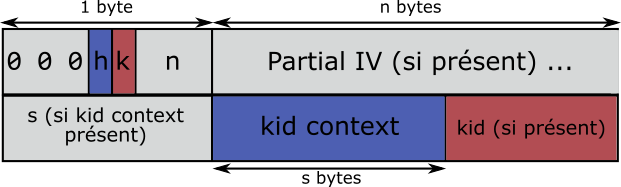
\includegraphics[width=0.9\textwidth]{OSCORE_option}
		\caption{Contenu de l'Option OSCORE}
		\label{fig:OSCORE_option}
	\end{minipage}\hfill
	\begin{minipage}{0.43\textwidth}
        \centering
        
		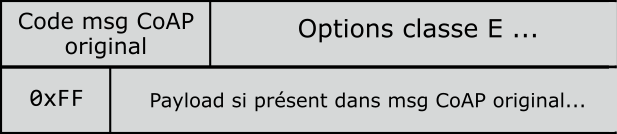
\includegraphics[width=0.9\textwidth]{OSCORE_plaintext}
		\caption{\textit{plaintext} inclus dans le COSE\_obj}
		\label{fig:OSCORE_plaintext}
	\end{minipage}	
\end{figure}

\subsubsection{Contextes de sécurité et échanges sur le canal OSCORE}
\label{OSCORE_contexts}

Un contexte de sécurité regroupe tout le matériel nécessaire à la sécurisation des échanges avec un hôte distant, pour une ressource donnée. OSCORE fait l'hypothèse que les deux hôtes partagent des paramètres pré-établis qui constituent le \textit{common context} (CC) : une clé dite \textit{Master Secret} (et optionnellement un \textit{Master Salt}), un vecteur d'initialisation \textit{Common IV} et quels sont les algorithmes précis à utiliser pour le procédé de dérivation de clés/chiffrement du COSE\_obj. De ce CC, sont ``dérivés" deux contextes distincts pour chaque hôte : le \textit{sender context} (SC) qui est utilisé pour protéger les messages à envoyer et le \textit{recipient context} (RC) utilisé pour déchiffrer les messages reçus. Ces contextes sont littéralement dérivés dans le sens où une fonction de dérivation de clés HKDF (\textit{HMAC-based Extract-and-Expand Key Derivation Function}, \cite{rfc5869}) construit, à partir du CC et d'un ID donné, une nouvelle clé spécifique au contexte en question. Dans le cas du SC, une \textit{sender key} (SK) et dans le cas du RC, une \textit{recipient key} (RC). L'ID en question est un nom (chaîne de caractères) qui désigne un hôte et est appelé \textit{sender ID} (SID) en association avec le SC et \textit{recipient ID} (RID) avec le RC. Il a une valeur arbitraire et est établi par un moyen non spécifié, mais un hôte doit avoir un SID pour envoyer un message (propre à lui-même) et un  RID pour valider un message reçu (propre à l'émetteur du message).\\

\par La \wordlink{Figure}{fig:OSCORE_plaintext} schématise l'utilisation des contextes dans un échange : il faut noter que pour un envoi de message le SC utilisé par l'émetteur contient le même matériel que le RC utilisé par le récepteur. Effectivement, ils doivent utiliser une clé identique pour la protection et la vérification de la ressource. Le terme ``récupération de contexte" désigne le fait que soit le contexte existe (déjà dérivé) et est récupérable depuis les éléments en substance, soit il est dérivé à la volée depuis le CC en utilisant les éléments en substance. Un élément non repris dans la \wordlink{Figure}{fig:OSCORE_plaintext} est le \textit{context ID} : inclus optionnellement dans l'option OSCORE, il permet de distinguer les contextes de sécurité et préciser lequel utiliser (à partir que quel CC dériver). Il permet l'utilisation d'un même SID interprétable dans des contextes distincts et est employé durant la procédure de join 6TiSCH. 
\vspace{0.1cm}

	\begin{figure}[!ht]
	\centering
	\includegraphics[width=0.9\linewidth]{OSCORE_contexts}
	\caption{Schéma fonctionnel d'un échange OSCORE et des contextes utilisés pour sécuriser le ``canal"}
	\label{fig:OSCORE_contexts}
	\end{figure}


\newpage

La \wordlink{Figure}{fig:OSCORE_scheme} établit que le champ \textit{ciphertext} du COSE\_obj contient, outre le plaintext, l'AAD (\textit{Additional Authenticated Data}) et le nonce AEAD. L'AAD désigne les données qui doivent être authentifiées mais rester lisibles, et donc répliquées dans le champ \textit{unprotected} du COSE\_obj. L'AAD est passé indépendamment du plaintext à l'algorithme AEAD, et est calculé comme un bytestream d'une structure \textit{Enc\_structure} \cite{rfc8152} dont le contenu est illustré par la \wordlink{Figure}{fig:OSCORE_AAD}. On y retrouve logiquement les Options catégorisées en classe I (vérification d'intégrité uniquement).
 
\vspace{0.2cm}
	\begin{figure}[!h]
	\centering
	\includegraphics[width=0.95\linewidth]{OSCORE_AAD}
	\caption{Détail de quels champs du paquet original et valeurs sont utilisés pour calculer l'AAD}
	\label{fig:OSCORE_AAD}
	\end{figure}
 
\vspace{0.4cm}
 
Le nonce AEAD est inclus dans toute Request émise par un client. Il permet de vérifier le partial IV qui a la valeur du Sender Sequence Number (CoAP) du client et qui est comparé avec la Replay Window du serveur. La Replay Window sert de parade aux attaques de types replay.
La construction du nonce AEAD (\wordlink{Figure}{fig:OSCORE_nonce}) est indirectement liée à la clé utilisée pour chiffrer le COSE\_obj, car le Common IV a été calculé en utilisant cette dernière. Il dépend également du SID du client et du partial IV. Ces éléments sont connus par le serveur à la réception de la Request, le Common IV étant dans le common context et l'Option OSCORE contenant le SID (valeur de \textit{kid}) et le PIV (voir \wordlink{Figure}{fig:OSCORE_option}). Le serveur peut donc calculer le nonce AEAD et le comparer à celui contenu dans le \textit{ciphertext} de la Request reçue. 
 
\vspace{0.2cm}

	\begin{figure}[!h]
	\centering
	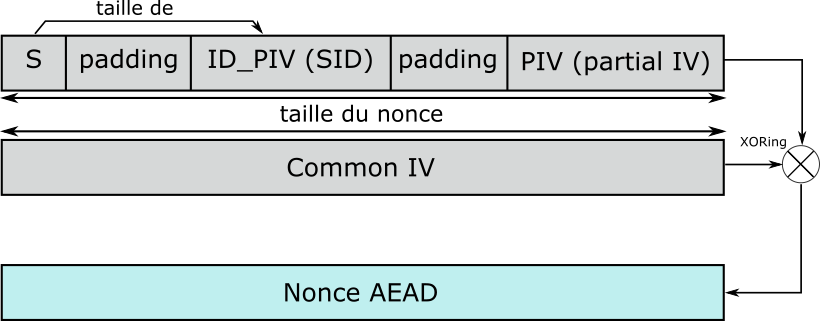
\includegraphics[width=0.75\linewidth]{OSCORE_nonce}
	\caption{Procédure de calcul du nonce AEAD à partir du PIV (=Sender Sequence Number)}
	\label{fig:OSCORE_nonce}
	\end{figure}

\vspace{0.6cm}

La \wordlink{Figure}{fig:OSCORE_exchange} résume un échange Request/Response protégé dans un canal OSCORE dans sa globalité : le dérivation des contextes, la formation et le chiffrement des messages OSCORE et la place du proxy dans cet échange. La spécification OSCORE \cite{rfc8613} est beaucoup plus complète, notamment au niveau des conditions/garanties de sécurité, mais n'offre pas une telle vue d'ensemble de tout le processus. 

\newpage


	\begin{figure}[!hb]
	\centering
	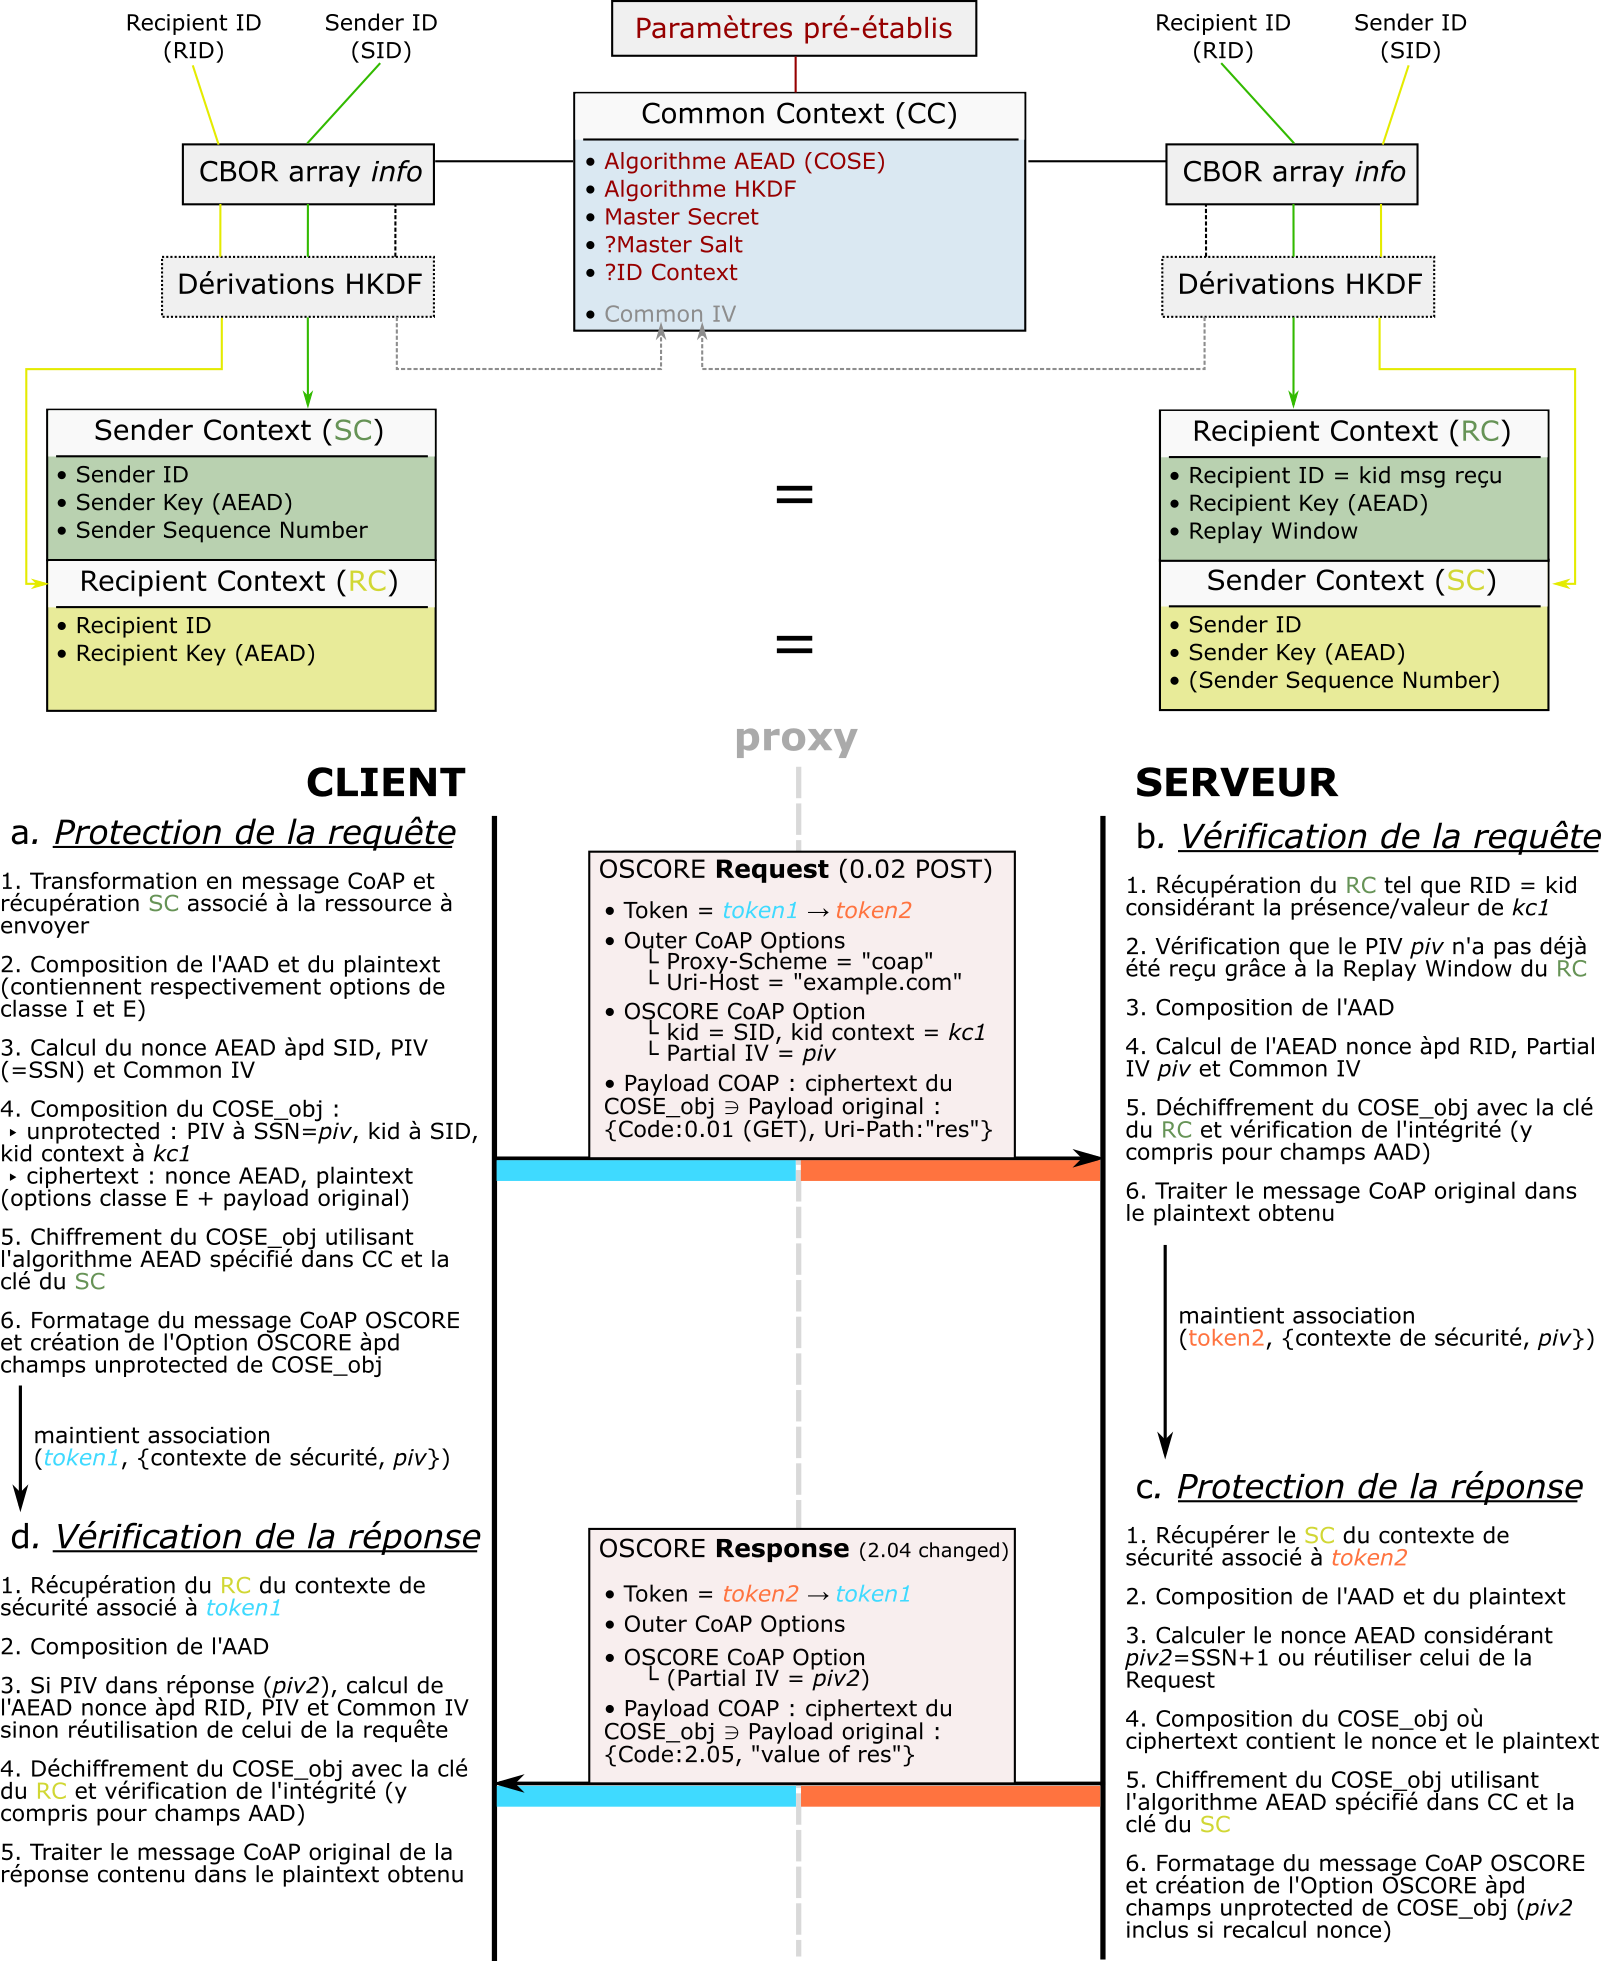
\includegraphics[width=\linewidth]{OSCORE_exchange}
	\caption{Vue d'ensemble d'un échange client-serveur protégé par OSCORE : dérivation des contextes, formation et procédure de chiffrement COSE des messages et place du proxy dans l'échange}
	\label{fig:OSCORE_exchange}
	\end{figure}

\newpage

\subsection{CoJP}
\label{CoJP}

Le protocole qui encadre la phase de join 6TiSCH est intégralement décrit par le WG 6TiSCH dans la spécification ``\texttt{Minimal Security Framework for 6TiSCH}" \cite{ietf-6tisch-minimal-security-15} qui est toujours en phase de draft. Il s'agit de CoJP (\textit{Constrained Join Protocol}) qui, comme introduit dans la \wordlink{Section}{intro_CoJP}, se repose sur CoAP, OSCORE et CBOR pour les échanges d'informations relatives au processus de join. Afin de répondre à des questions de mise en pratique des standards 6TiSCH et particulièrement de la phase de join et de sa configuration, le standard ``\texttt{Minimal IPv6 over the TSCH Mode of IEEE802.15.4e (6TiSCH) Configuration}" \cite{rfc8180} est utilisé. Dans le reste de ce chapitre, les éléments de ce standard sont considérés et employés de façon transparente quand la spécification \cite{ietf-6tisch-minimal-security-15} ne les précise pas directement, celle-ci faisant certaines abstractions vis-à-vis de la mise en pratique.\\

La phase de join permet le join sécurisé d'un nouveau nœud à un réseau 6TiSCH déjà établi. Le terme de ``join sécurisé" réfère à un accès authentifié au réseau et la distribution des paramètres de configuration nécessaires au nœud pour intégrer le réseau (clés, identifiants, etc.). Dans le cadre de la joining phase, les acteurs sont les suivants (illustrés dans la \wordlink{Figure}{fig:joining_phase_network}) :
\vspace{0.1cm}
\begin{itemize}[label=$\bullet$]
\item le \textit{\textbf{pledge}} : un nœud 802.15.4 qui souhaite rejoindre le réseau 6TiSCH, dont l'EUI-64 est désigné ici par \textit{pledgeID}
\item le \textbf{JRC} (\textit{Join Registrar/Coordinator}) : une entité centrale qui a autorité sur le réseau 6TiSCH, mais pouvant être située à son extérieur dans un backbone.
\item le \textbf{JP} (\textit{Join Proxy}) : le pledge n'ayant pas un accès direct au JRC, il a besoin d'un nœud intermédiaire déjà membre du réseau pour acheminer ses messages vers ce dernier. Un join proxy effectue se travail, agissant comme un proxy au niveau applicatif (CoAP). 
\item le \textit{\textbf{joined node}} : terme désignant un pledge qui vient de finaliser avec succès son join sécurisé.
\item le \textbf{6LBR} (\textit{6LoWPAN Border Router}) : nœud faisant la jonction entre le réseau WSN 6TiSCH et le backbone (illustré dans la \wordlink{Section}{archWSN}), supposé comme étant la racine de l'arborescence RPL 
\end{itemize}

	\begin{figure}[!h]
	\centering
	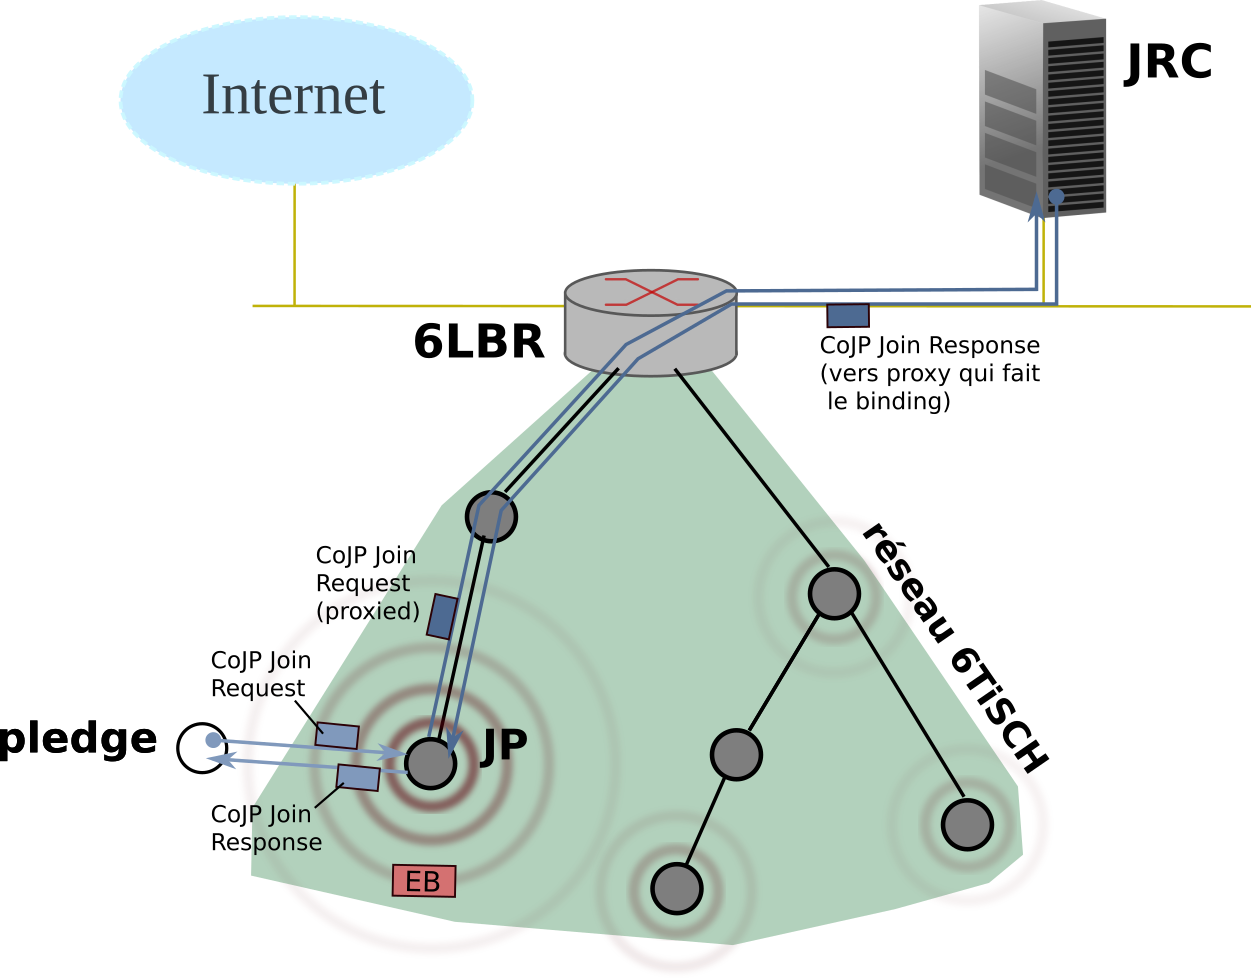
\includegraphics[width=0.73\linewidth]{Joining_phase_network}
	\caption{Place dans le réseau des différents acteurs de la phase de join}
	\label{fig:joining_phase_network}
	\end{figure}


\newpage

\subsubsection{Problématiques liées à la joining phase}

La joining phase est critique dans la création et le maintient de la stabilité d'un réseau 6TiSCH. À noter que ce réseau reste un réseau 802.15.4 et est donc vu au niveau lien comme une structure PAN. La joining phase encadre notamment les problématiques suivantes :
\vspace{0.2cm}
\begin{enumerate}
\item Un pledge n'a aucune connaissance du réseau, si ce n'est certains paramètres pré-établis. Il doit obtenir des éléments essentiels tels que les clés courantes utilisées pour protéger le trafic au niveau lien, un identifiant dans le réseau (sous-entendu une short address), l'adresse IPv6 du JRC et un parent RPL.
\vspace{0.2cm}
\item Les paramètres fournis à un joined node peuvent changer au cours du temps. Par exemple, en cas de rekeying du réseau suite à une détection d'attaque. Il convient de redistribuer les nouveaux paramètres de façon consistante.
\vspace{0.2cm}
\item Le pledge doit pouvoir s'authentifier auprès du JRC et communiquer de façon sécurisée avec ce dernier. Des paramètres sont pré-établis à ces fins (pour communiquer sur un canal OSCORE) mais la façon dont ceux-ci sont distribués au pledge et JRC de manière concordante n'est pas précisée.
\vspace{0.2cm}
\item Le mode TSCH implique qu'un pledge n'a à priori aucune idée de quand et sur quel canal écouter à la recherche d'EB qui lui permette d'initier le processus de join. Il s'agit donc d'un scan passif qui coûte cher au pledge énergétiquement parlant.
\vspace{0.2cm}
\item Les microcontrôleurs constituant les nœuds de WSNs ont un espace mémoire limité, le processus de join ne devrait pas faire intervenir de nouvelles technologies ou protocoles qui ne sont pas déjà utilisés de façon générique dans 6TiSCH.
\end{enumerate}

\subsubsection{Hypothèses faites par CoJP (paramètres pré-établis)}
\label{preshared_join}

La spécification \cite{ietf-6tisch-minimal-security-15} fait l'hypothèse que certains paramètres sont pré-établis, pour le pledge et le JRC. Cela peut se faire physiquement par une interface JTAG, une console, \textit{over-the-air} dans une cage de Faraday, etc. ou en utilisant par exemple un protocole d'échange de clés. Ces \textbf{paramètres pré-établis} sont les suivants (ceux qui sont optionnels sont notés entre [..]) :
\vspace{0.2cm}
\begin{itemize}[label=$\bullet$]
\item identifiant du pledge (\textit{pledgeID}) : doit être unique parmi l'ensemble des nœuds sur lequel le JRC a autorité. Typiquement mis à l'EUI-64 qui est globalement unique et attribué d'office à une interface 802.15.4 (dérivé de l'adresse MAC). Peut aussi être issu d'un autre procédé de génération qui respecte l'unicité.
\vspace{0.2cm}
\item une clé partagée (\textit{PSK}, \textit{Pre-Shared Key}) : une clé secrète partagée entre le pledge et le JRC, ce dernier doit de ce fait stocker quelle clé est assignée à chaque \textit{pledgeID}. Ces clés doivent être cryptographiquement fortes (minimum 128 bits, générées aléatoirement). Un travail portant sur l'échange préliminaire sécurisé des clés utilisables par OSCORE est en cours de standardisation, désigné par LAKE (\textit{Lightweight Authenticated Key Exchange protocol}, \cite{ietf-lake-reqs-03}).
\vspace{0.2cm}
\item {[} un identifiant de réseau (\textit{netwID}) ] : identifie le réseau 6TiSCH, annoncé dans les EBs émis par les nœuds qui en font déjà partie. Il s'agit typiquement du PAN ID. S'il n'est pas fourni à un pledge, celui-ci tentera de rejoindre n'importe quel réseau sans distinction.
\vspace{0.2cm}
\item {[} les algorithmes différant de ceux par défaut ] : si non spécifiés, la spécification \cite{ietf-6tisch-minimal-security-15} définit quel algorithme  utiliser pour quelle action par défaut (actions relatives à la sécurité).
\vspace{0.2cm}
\item Pour un pledge qui aspire à servir de 6LBR, l'adresse IPv6 GUA du JRC : permet au pledge de contacter directement le JRC sans utiliser de nœud intermédiaire (par son interface vers le backbone). Un pledge normal l'apprend dynamiquement au cours du processus de join.
\end{itemize}

\newpage

\subsubsection{Composants du protocole CoJP et leur sécurisation}
\label{CoJP_components}

Dans cette sous-section, les mécanismes et éléments propres au protocole CoJP sont décrits. Le déroulement de la phase de join dans sa globalité et l'utilisation de CoJP durant celle-ci sont détaillés dans la \wordlink{Section}{join_phase_analysis}. CoJP définit deux échanges de messages distincts (illustrés par la \wordlink{Figure}{fig:joining_phase_simplified}) :
\vspace{0.3cm}
\begin{enumerate}
\item \textit{Join Exchange} : celui inclus dans la phase de join à proprement parler. C'est dans cet échange que sont transportés 
	\begin{enumerate}
	\item la demande de join émise par le pledge vers le JRC (proxied par le JP qui est le seul nœud que peut atteindre le pledge)
	\item la réponse du JRC en fonction de la demande du pledge, du JRC vers le pledge (vers le JP en fait, qui relaie en sa qualité de proxy vers le pledge)
	\end{enumerate}
\vspace{0.2cm}	
\item \textit{Parameter Update Exchange} : ne fait pas partie du join en lui-même, mais est initié par le JRC vers un joined node pour mettre à jour des paramètres qui lui avaient été transmis lors du join exchange (par exemple en cas de rekeying du réseau). Le joined node répond avec une réponse vide qui permet au JRC de s'assurer de la bonne réception de l'update. Aucun proxy applicatif ne doit intervenir ici car le nœud a déjà rejoint le réseau.
\end{enumerate} 
\vspace{0.3cm}

Dans ces échanges, l'information est transportée comme du payload applicatif CoAP, sous la forme d'objets CBOR. La spécification \cite{ietf-6tisch-minimal-security-15}  en définit deux : les objets \textit{Join\_Request} et \textit{Configuration}, dont le contenu essentiel est brièvement énuméré dans les messages de la \wordlink{Figure}{fig:joining_phase_simplified}. L'objet Join\_Request est destiné à recevoir les paramètres que le pledge veut communiquer au JRC pour accompagner sa demande d'intégration au réseau. L'objet \textit{Configuration} est destiné à recevoir les paramètres de configuration actuellement en vigueur dans le réseau, donnés par le JRC qui doit les fournir à un pledge pour permettre son intégration. La sémantique des champs que contiennent ces objets est décrite ci-dessous (ceux qui sont facultatifs sont entourés de [..]).\\

\vspace{0.2cm}
\noindent\textit{Join\_Request} (pledge $\rightarrow$ JRC) : 
\begin{itemize}[label=$\bullet$]
\item {} [ role ] : rôle désiré par le pledge dans le réseau (\texttt{6TiSCH node} ou \texttt{6LBR})
\item {} [ netwID ] : identifiant du réseau 6TiSCH que le pledge désire rejoindre (un JRC peut faire autorité sur plusieurs réseaux 6TiSCH en même temps)
\item {} [ unsupported configuration ] : utilisé dans la gestion de conflits de configuration, non détaillée dans ce document
\end{itemize}

\vspace{0.3cm}
\noindent\textit{Configuration} (JRC $\rightarrow$ pledge/joined node) : 
\begin{itemize}[label=$\bullet$]
\item link-layer key set : tableau d'objets \textit{Link\_Layer\_Key} où chacun décrit une clé utilisée au niveau lien et son usage (non détaillé ici)
\item {} [ short identifier ] : objet \textit{Short\_Identifier} qui reprend l'identifiant attribué par le JRC (unique) et le temps de validité de ce dernier
\item {} [ JRC address ] : l'adresse IPv6 GUA du JRC, de sorte que le pledge, une fois joined node, puisse s'adresser directement à ce dernier (et servir de JP)
\item {} [ blacklist ] : tableau de short identifiers dont le JRC ne souhaite pas l'acceptance des frames par le pledge (une fois qu'il deviendra joined node), permet par exemple d'isoler des noeuds corrompus ou non désirés par l'autorité que constitue le JRC
\item {} [ join rate ] : débit maximum de trafic de join en \textit{bytes/s} que le pledge, une fois joined node et endossant le rôle de JP, peut forward vers l'intérieur du réseau (drop des paquets excédants)
\end{itemize}

\newpage

	\begin{figure}[!ht]
	\centering
	\includegraphics[width=\linewidth]{joining_phase_simplified}
	\caption{Vue d'ensemble de la joining phase et de la mise à jour des paramètres distribués par CoJP}
	\label{fig:joining_phase_simplified}
	\end{figure}

\vspace{0.3cm}

La sécurité du contenu des échanges CoJP (niveau applicatif donc) s'appuie intégralement sur OSCORE. C'est pourquoi CoJP fait l'hypothèse qu'une PSK est connue initialement des deux côtés de l'échange : le pledge et le JRC doivent pouvoir dériver des contextes de sécurité qui se correspondent. Les détails de quelles valeurs sont utilisées pour les différents paramètres durant la dérivation sont explicités plus loin. Le canal sécurisé établi par OSCORE permet d'assurer, par les propriétés de ce dernier, la confidentialité, l'authenticité des données et une protection contre les rejeux. Il s'agit bien d'une protection au niveau applicatif, tout en permettant le proxying par le JP détaillé dans la section suivante. Au niveau lien, le pledge n'ayant aucune connaissance des clés utilisées dans le réseau, il n'y a aucune protection appliquée pour les échanges entre le pledge et le JP. En revanche, le JP étant un joined node, il a connaissance des clés et toutes les frames échangées entre le JP et le JRC (multi-hop possible, voir \wordlink{Figure}{fig:joining_phase_network}) sont sécurisées au niveau lien avec ces clés. La \wordlink{Figure}{fig:joining_phase_simplified} illustre schématiquement les échanges CoJP et à quel niveau s'appliquent ces chiffrements/authentifications. À noter qu'une fois un pledge devenu joined node, les échanges qu'il peut avoir par la suite avec le JRC utiliseront toujours le même contexte de sécurité OSCORE, mais ne feront plus intervenir de JP en plus d'être intégralement protégés au niveau lien.

\newpage

\subsubsection{Join Exchange CoJP et Join Proxy}
\label{join_exchange_CoJP}

Au moment d'initier le Join Exchange CoJP, un pledge dispose d'informations qu'il a reçues du nœud qui va servir de Join Proxy (JP). Au niveau lien (TSCH), le pledge est synchronisé temporellement et a connaissance des cells qu'il peut utiliser pour les échanges durant la joining phase (information issue de l'EB reçu). Au niveau réseau, le pledge utilise son adresse Link-Local après s'être assuré qu'elle est unique. L'obtention de ces informations est décrite dans la \wordlink{Section}{global_EB}. Il s'apprête donc à envoyer sa Join Request (CoJP) vers le JP.\\


 Le pledge et le JRC protègent le contenu applicatif échangé avec le matériel issu du contexte de sécurité, dérivé comme décrit par la \wordlink{Section}{OSCORE_contexts} et à partir des paramètres pré-établis donnés à la \wordlink{Section}{preshared_join}. Il en résulte un contexte de sécurité OSCORE où sont connus :
 \vspace{0.1cm}
\begin{itemize}[label=$\bullet$]
\item \textit{Master Secret} = PSK

\item \textit{Master Salt} = \texttt{""} (chaîne vide)

\item \textit{ID Context} = identifiant unique du pledge que le JRC doit considérer pour décider de si le pledge est autorisé dans le réseau (\textit{pledgeID}, vraisembablement son EUI-64), transmis dans le champs \textit{kid context} 

\item Le nom identifiant un pledge de façon générique dans la communication OSCORE est la chaîne vide \texttt{""}, il sera utilisé comme Sender ID dans l'envoi de message par le pledge (et donc dans la dérivation du Sender Context pour le pledge).

\item Le nom identifiant le JRC dans la communication OSCORE est la chaîne \texttt{"JRC"} et il sera utilisé comme Recipient ID \textbf{par le pledge}, et donc dans la dérivation du Recipient Context utilisé par la suite quand une réponse sera reçue.

\item L'Algorithme AEAD est supposé être \texttt{AES-CCM-16-64-128}, sauf si un autre algorithme a été pré-établi (voir algorithmes supportés par COSE, \cite{rfc8152})

\item La fonction de dérivation de clés (HKDF) est supposée être \texttt{HKDF SHA-256}, sauf si une autre fonction a été pré-établie (voir algorithmes de dérivation définis pour COSE, \cite{rfc5869} et \cite{rfc5869}).
\end{itemize}

\vspace{0.1cm}

\minit{pledge $\rightarrow$ JP (Join Request)}

La Join Request émise par le pledge contient un objet Join\_Request indiquant quel réseau il souhaite rejoindre (\textit{netwID}) et le rôle qu'il souhaite y endosser : 6LBR ou nœud régulier. Le cas 6LBR correspond au cas spécial où le pledge veut en fait être la racine d'un nouveau réseau (et donc ne passe pas par un JP), il n'est pas traité ici. Le détail de la Join Request est donné par la \wordlink{Figure}{fig:join_request}. Elle est protégée par OSCORE, le pledge ayant utilisé son Sender Context pour cela, et donc la Sender Key qu'il contient. L'Option OSCORE est construite avec le champ \textit{kid} prenant la valeur du SID, donc une chaîne vide puisque c'est le pledge qui envoie. Cependant, afin que le JRC puisse récupérer le contexte associé au pledge (contenant la PSK qu'il partage avec), il a besoin de savoir de quel pledge il s'agit. C'est pourquoi le champ \textit{kid context} de l'Option OSCORE prend la valeur de l'ID Context, qui est l'identifiant du pledge. Le pledge maintient en mémoire l'association entre la valeur du token créé et le contexte de sécurité.\\

 Le JP accepte la frame contenant la Join Request bien qu'elle ne soit pas sécurisée, en mettant un flag 802.15.4 ``\texttt{secExempt}" associé au pledge dans la table des voisins (\wordlink{Section}{neighbors_table}). Il a alors accès aux informations que OSCORE ne chiffre pas et va effectuer son rôle de proxy en consommant les Options qui s'y rapportent. Le proxy va opérer son rôle en mode \textit{stateless}. Un proxy stateless CoAP \cite{ietf-core-stateless-05} compresse l'information dont il a besoin pour relayer la future réponse, dans le token CoAP du message même qu'il relaie. Effectivement, la future réponse référençant la même valeur de token, le JP pourra donc en retirer ce dont il a besoin pour acheminer vers le pledge : adresse IPv6 du pledge et port UDP source. Cette technique utilise des tokens de taille étendue (spécification \cite{ietf-core-stateless-05}) et permet de sauvegarder de la mémoire (état maintenu dans les messages eux-mêmes et non par le JP) et d'éviter par ce biais des attaques de déni de service.\\
 
 Outre le fait d'agir comme un stateless proxy en créant un nouveau token dépendant de l'état à stocker, le JP va effectuer son rôle de proxy normal. Le pledge ayant renseigné le nom d'hôte générique pour désigner le JRC \texttt{"6tisch.arpa"}, le proxy va le résoudre en l'adresse IPv6 GUA du JRC qu'il connaît, lui. Il va également mettre le message CoAP à \textit{NON} à la place de \textit{CON} (expliqué à la \wordlink{Section}{join_secu}).\\

\newpage

\vspace{0.2cm}
	\begin{figure}[!h]
	\centering
	\includegraphics[width=\linewidth]{Join_Request}
	\caption{Forwarding d'une Join Request par un Join Proxy}
	\label{fig:join_request}
	\end{figure}
\vspace{0.2cm}

\minit{JP $\rightarrow$ JRC (Join Request)}

La Join Request transite dans le réseau 6TiSCH, en plusieurs sauts vraisembablement, vers le 6LBR qui lui-même la relaie vers le backbone où se trouve le JRC. Il est également possible que les fonctions de 6LBR et JRC soient co-situés et sont en fait le même hôte. Un fois la Join Request parvenue au JRC, ce dernier récupère le contexte de sécurité associé au pledge. Celui-ci contient la PSK partagée avec le pledge et le Master Salt entre autres (voir début de \wordlink{Section}{join_exchange_CoJP}). Le Recipient Context est calculé considérant le RID prenant la valeur du nom désignant le JRC \texttt{"JRC"} (puisque c'est le JRC qui reçoit). La Recipient Key obtenue permet de déchiffrer et vérifier le payload, qui est l'objet CBOR Join\_Request.\\

Le JRC traite la demande d'intégration du pledge en tenant compte de quel réseau il veut rejoindre, et de si ce dernier y est autorisé (détails propres à au déploiement). Si c'est le cas, il va alors lui attribuer un identifiant \textit{shortID} dans ce réseau, qu'il sait unique car il gère toutes les demandes d'intégration pour ce réseau. Il va également inclure dans sa réponse les clés au niveau lien qui y sont d'application à ce moment là, sa propre adresse IPv6 GUA, ainsi que d'autres paramètres (voir \wordlink{Section}{CoJP_components}), le tout étant placé dans les champs adéquats de l'objet CBOR Configuration. Ce dernier sera le payload de la Join Response.\\

\minit{JRC $\rightarrow$ JP (Join Response)}

Le JRC a protégé la Join Response avec le Sender Context, obtenu du contexte de sécurité dérivé à la réception de la Join Request. Il a été calculé en considérant un SID à la valeur de l'ID du JRC (\texttt{"JRC"}) puisque c'est ce dernier qui envoie. Le paquet transite jusqu'au JP, toujours en étant protégé au niveau lien car on reste dans le réseau 6TiSCH.\\

Le JP reçoit la Join Response et reconstruit l'état à partir du token CoAP qu'elle contient (voir \wordlink{Figure}{fig:join_response}). De cet état, il a les informations nécessaires pour acheminer le message vers le pledge.\\


\minit{JP $\rightarrow$ JRC (Join Response)}

 Au niveau applicatif, le seul changement concerne le type de message qui passe de \textit{NON} à \textit{CON}. Le JP relaie la Join Response dans une frame à destination du pledge. À noter que cette frame n'est alors pas sécurisée au niveau lien. De ce fait, si OSCORE n'était pas utilisé (sans être remplacé par une sécurité niveau transport), n'importe quel nœud pourrait voir en clair quelles sont les clés du réseau communiquées par le JRC. \\

\newpage


\vspace{0.2cm}
	\begin{figure}[!h]
	\centering
	\includegraphics[width=\linewidth]{Join_Response}
	\caption{Forwarding d'une Join Response par un Join Proxy}
	\label{fig:join_response}
	\end{figure}
\vspace{0.2cm}

Se basant sur la valeur du token dans le message CoAP reçu (qui doit être identique à celui de la Request), le pledge récupère le contexte de sécurité qui avait été initialement dérivé. Il se sert du Recipient Context obtenu de ce dernier et de la Recipient Key référencée dedans pour vérifier/déchiffrer la Join Response. Une fois l'objet Configuration obtenu, le pledge installe ce qu'il contient pour intégrer le réseau. Alors en possession de la GUA du JRC et des clés courantes du réseau, il sera également désormais à même de servir de JP pour un autre nœud. À cette fin, il commencera à émettre des EBs annonçant le réseau qu'il a rejoint.

\newpage

\section{Analyse du déroulement de la phase de join}
\label{join_phase_analysis}

\subsection{Procédure dans sa globalité}
La phase de join comprend deux étapes distinctes. La première, l'étape de scanning/advertising, correspond à la recherche d'EB par le pledge, sa synchronisation temporelle au niveau lien (TSCH) et éventuellement un échange IPv6 Neighbor Discovery entre le pledge et le JP. La seconde est l'étape d'intégration au réseau proprement dite, où le Join Exchange CoJP est effectué. Si le pledge est accepté, il reçoit alors le matériel nécessaire au niveau lien pour intégrer le réseau 6TiSCH et y communiquer. Il devra alors lancer les procédures pour se placer dans la topologie RPL et pour obtentir une adresse globale IPv6.\\

On considère ici un déploiement tel que supposé dans la spécification \cite{rfc8180} : 
\begin{itemize}[label=$\bullet$]
\item Deux clés son utilisées au niveau lien dans le réseau 6TiSCH : \textit{K1} est utilisée pour authentifier les EBs, \textit{K2} pour authentifier et chiffrer les frames normales et ACKs.
\item Le minimal schedule utilisé pour les communications relatives au processus de join (dit \textit{join schedule}) est composé de la seule cell (0, 0) en mode TxRxS (accueille tout le trafic broadcast de manière générale).
\item Pledge et JRC disposent des paramètres pré-établis relatifs à CoJP sur OSCORE (voir \wordlink{Section}{join_exchange_CoJP})
\end{itemize}

\subsubsection{Étape de scanning/advertising (EBs) et obtention d'adresse IPv6}
\label{global_EB}

Le déroulement de cette étape décrit textuellement ci-dessous est synthétisé par la \wordlink{Figure}{fig:join_part1}.\\

Le pledge, une fois prêt à entamer son intégration au réseau, va chercher à capter des EBs émis par des joined nodes des potentiellement différents réseaux 6TiSCH à portée. Il n'y a pas de technique particulière énoncée dans les standards pour encadrer la façon dont le pledge doit procéder, que ce soit sur l'écoute de canal ou le nombre d'EBs dont il pourrait attendre la réception pour comparaison avant de lancer la suite du processus. La comparaison d'EBs peut se faire sur plusieurs critères. La \wordlink{Section}{EBs} introduisait brièvement le contenu d'un EB pour TSCH, le draft \cite{ietf-6tisch-enrollment-enhanced-beacon-14} y apporte une structure supplémentaire contenant divers champs, dont certains sont utiles dans la discrimination entre EBs.\\

Le processus discriminatoire peut se baser sur les critères suivants ($\triangleright$ pour ceux basés sur \cite{ietf-6tisch-enrollment-enhanced-beacon-14})  :
\begin{itemize}[label=$\bullet$]
\item La Join Metric (de l'IE TSCH Synchronization), valeur dans [\texttt{0x00}, \texttt{0xFF}] issue d'une normalisation du rang RPL du noeud émetteur (voir \cite{rfc8180}). Une valeur plus faible indique une proximité avec la racine de l'arborescence et donc une préférence dans le fait de servir de parent.
\vspace{0.1cm}
\item Le PAN ID du PAN auquel l'annonceur appartient ou l'adresse lien du noeud annonceur (source de l'EB).
\item La force du signal avec lequel l'EB a été reçu.
\end{itemize} 
\begin{itemize}[label=$\triangleright$]
\item La Proxy Priority dont une valeur moins élevée dans l'intervalle [\texttt{0x00}, \texttt{0x7e}] indique une bonne capacité à supporter du trafic non chiffré et une disponibilité des ressources (places dans la cache, etc.).
\vspace{0.1cm}
\item La PAN Priority dont une valeur moins élevée indique la propension à recevoir de nouveaux noeuds, comparable d'un PAN à l'autre.
\vspace{0.1cm}
\item Le Network ID tel que défini dans \cite{ietf-6tisch-enrollment-enhanced-beacon-14}, plutôt relatif à un ensemble de PANs qu'à un seul en particulier : valeur arbitraire qui peut être calculée comme un hash du préfixe /64 du réseau.
\end{itemize}
\vspace{0.4cm}

Une fois un EB sélectionné, le pledge doit se synchroniser temporellement avec le noeud qui l'a émis et qui servira de JP. L'EB contient l'IE \textit{TSCH Timeslot} qui donne l'ID du template de l'organisation des transmissions dans un timeslot (voir \wordlink{Section}{templatetimeslot}) duquel peut être déduit \textit{TsTxOffset}, c'est-à-dire le temps écoulé depuis le début du timeslot à l'instant du début d'émission de la frame. Possèdant le timestamp de la réception de l'EB, le pledge est alors capable de se calquer sur les timeslots utilisés par le réseau. L'IE \textit{TSCH Synchronization} donne l'ASN, l'IE \textit{Channel Hopping }identifie la séquence des fréquences utilisées et finalement l'IE \textit{TSCH Slotframe and Link }donne l'initial schedule que le JP considère pour le trafic de join (le pledge doit donc le suivre). Cette slotframe est donc installée par le pledge qui sait désormais quand se réveiller pour communiquer.\\

\newpage

\vspace{0.2cm}
	\begin{figure}[!h]
	\centering
	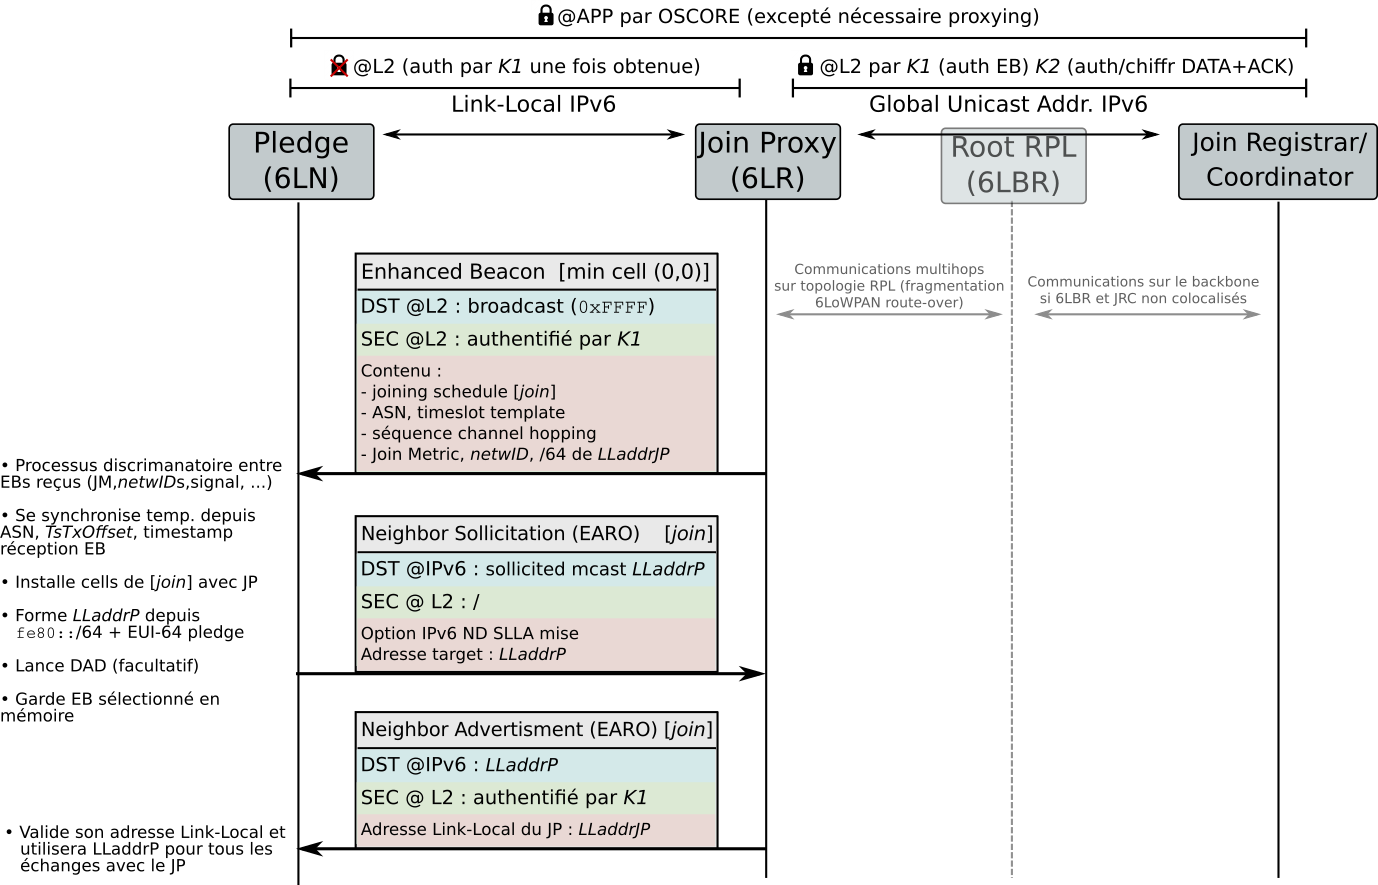
\includegraphics[width=\linewidth]{Joining_phase_part1}
	\caption{Réception d'EB et validation de l'adresse IPv6 du pledge}
	\label{fig:join_part1}
	\end{figure}
\vspace{0.2cm}

Le pledge doit connaître l'adresse Link-Local du JP que ce dernier souhaite qu'il utilise pour le reste de la joining phase. À priori elle peut être dérivée par le pledge depuis la long address indiquée comme source de l'EB, mais elle peut aussi être spécifiée dans l'EB même (champ Join Proxy Interface ID de \cite{ietf-6tisch-enrollment-enhanced-beacon-14}).\\

Le pledge va former et utiliser son adresse Link-Local IPv6 pour le reste de la phase de join. Il le fait à partir de son \textit{pledgeID}, qui est vraisembablement son EUI-64 et du préfixe connu \texttt{fe80::}/64. Si c'est le cas, il peut se passer de l'échange suivant qui est le Neighbor Discovery IPv6 avec le JP, car l'EUI-64 est supposé unique. Sinon, il peut y avoir un échange de messages Neighbor Solicitation/Neighbor Advertisment afin de valider l'unicité de l'adresse Link-Local employée par le pledge pour le reste du processus de join.\\

Ces échanges ne sont couverts par aucune garantie en terme de sécurité, le pledge agit comme s'il pouvait avoir confiance en l'EB reçu du Join Proxy. Cependant, il est notable que dans la \wordlink{Figure}{fig:join_part1}, les messages émis par le JP sont quand même authentifiés par la clé K1. Ce sera utile au pledge pour vérifier plus tard, une fois le keying material du réseau reçu, que l'EB sur lequel il a basé sa synchronisation était conforme (développé dans la \wordlink{Section}{join_secu}). 

\newpage

\subsubsection{Étape d'intégration au réseau (échange CoJP) et opérabilité RPL}
\label{global_CoJP}

L'échange CoJP peut alors être initié par le pledge, schématisé par la \wordlink{Figure}{fig:join_part2}. La dérivation des contextes de sécurité OSCORE et le contenu des messages est tel que décrit par la \wordlink{Section}{join_exchange_CoJP}. Les messages échangés entre le pledge et le JP le sont toujours en utilisant le join schedule, tandis ce que entre le JP et le JRC il s'agit de cells arbitraires qui peuvent être le résultat de négociations 6top.\\

Le JP accepte les frames en provenance du pledge et ce même si elles ne sont pas sécurisées. La spécification \cite{ietf-6tisch-minimal-security-15} précise que cela peut se faire en mettant un flag \texttt{"secExempt"} associé au pledge dans les tables utilisées par 802.15.4. En revanche, elle ne précise pas comment le JP détecte que le message issu du pledge est une Join Request. Les communications entre le JP et le JRC sont protégées au niveau lien par les clés \textit{K1} et \textit{K2}. Ce sont ces clés que le JRC écrit dans l'objet \textit{link\_layer\_key\_set} de l'objet Configuration renvoyé dans la Join Response.

\vspace{0.2cm}
	\begin{figure}[!h]
	\centering
	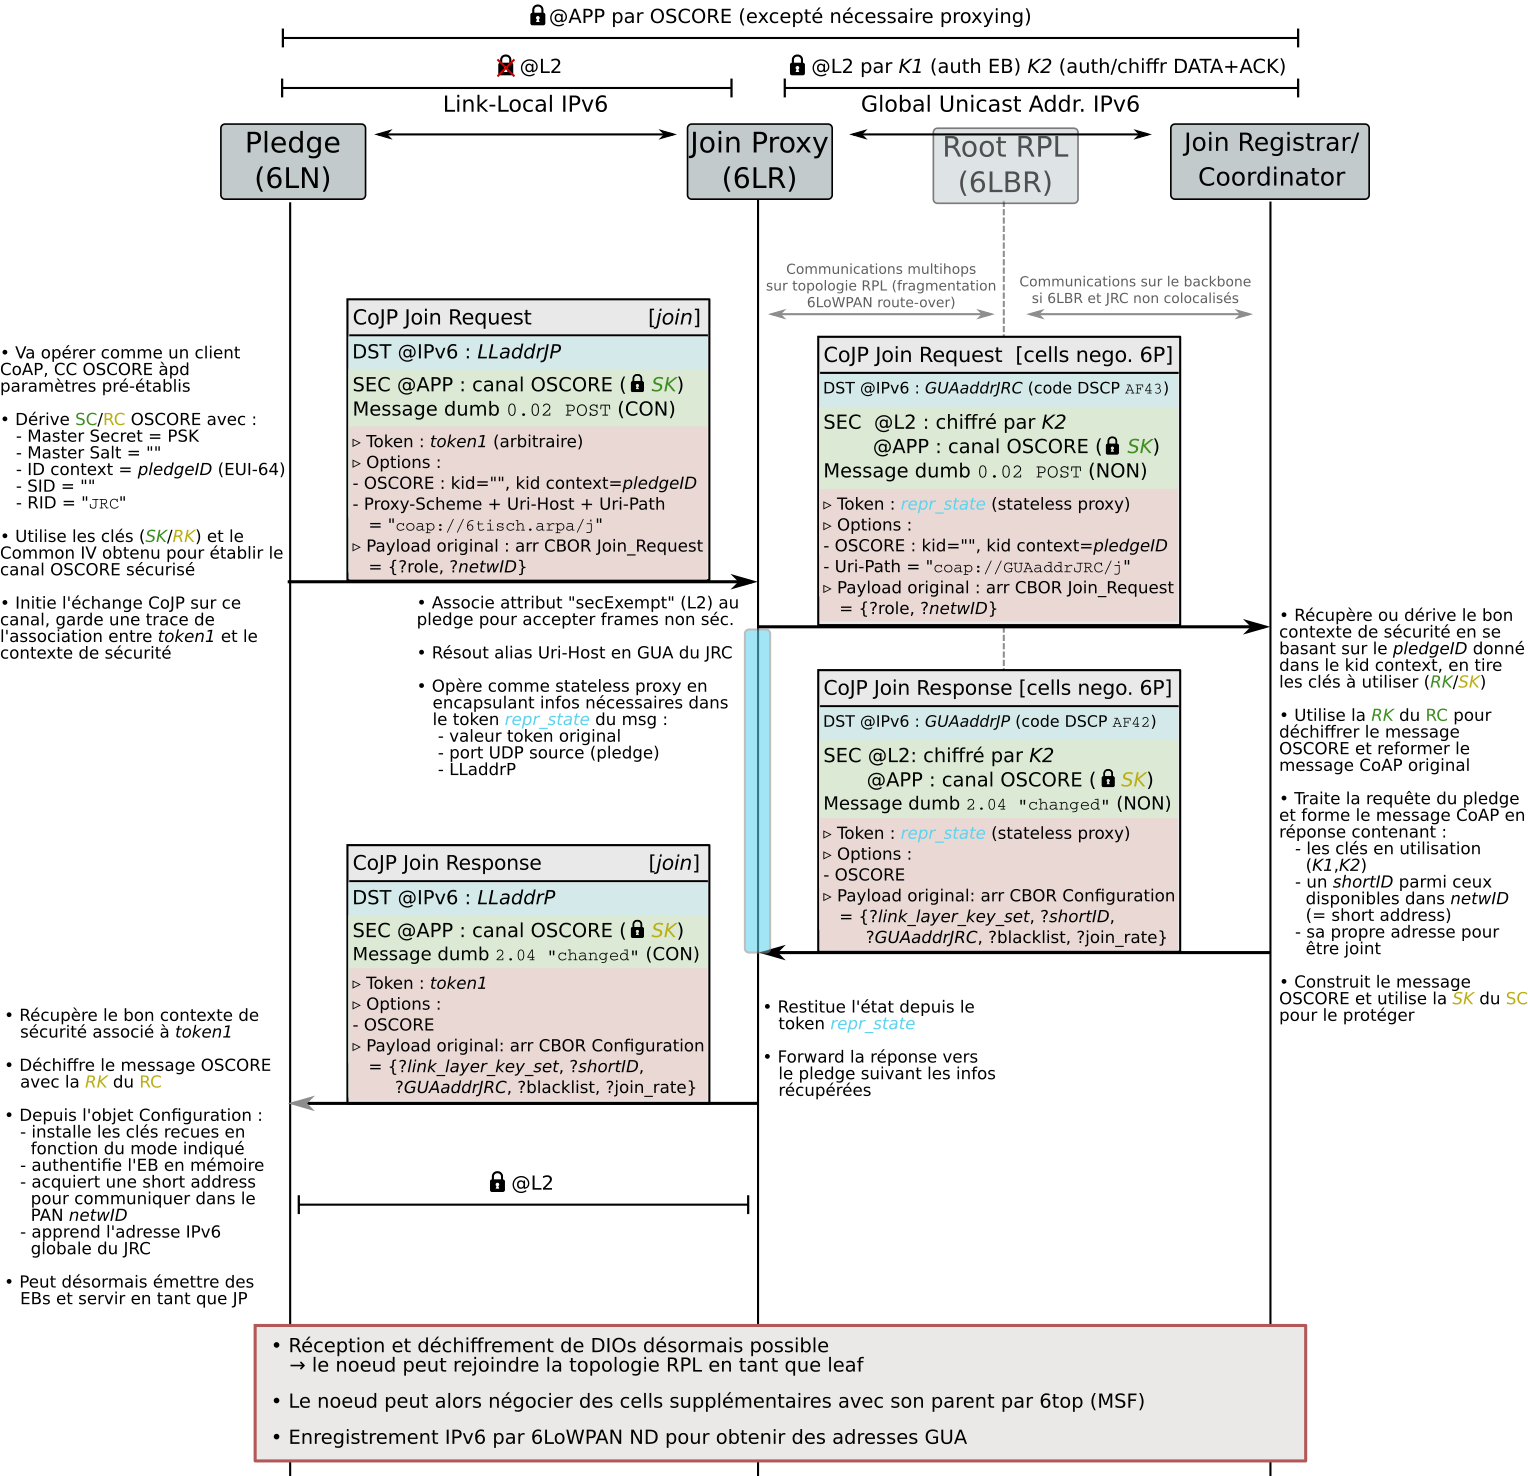
\includegraphics[width=\linewidth]{Joining_phase_part2}
	\caption{Échange CoJP menant à l'intégration au réseau du pledge}
	\label{fig:join_part2}
	\end{figure}
\vspace{0.2cm}

\newpage

Une fois le contenu de l'objet Configuration installé par le pledge, il est considéré comme intégré au réseau (joined node) dans le sens où il peut comprendre et vérifier les frames échangées, et en envoyer lui-même. Il peut également vérifier l'intégrité de l'EB qui lui a initialement permis de lancer le processus de join (voir \wordlink{Section}{join_secu}). Une fois effectué, le désormais joined node devrait idéalement pouvoir servir de JP s'il en a les capacités. Pour cela, il doit encore se situer dans la topologie RPL et obtenir une adresse globale IPv6 à partir du préfixe attribué au réseau. De plus, comme le joined node peut désormais envisager du trafic unicast avec d'autres noeuds du réseau, il ne devrait plus utiliser le minimal schedule (sauf pour le trafic purement broadcast) mais installer des cells spécifiques à ses voisins. Les négociations de ces cells peuvent se faire par 6top et sont gérées par la Scheduling Function en activité pour le joined node. Considérant qu'il s'agit de la MSF, le noeud devra d'abord s'être positionné dans la topologie RPL car les cells installées en dépendent.\\

Le joined node est maintenant capable de déchiffrer les DIOs émis en broadcast, gouvernés par le Trickle Timer RPL aux autres noeuds de la topologie (voir \wordlink{Section}{RPL}). Il peut en avoir stocké s'il en a reçu pendant que le processus de join était en cours, mais également solliciter les noeuds à portée avec un DIS. Il en tire un ensemble de noeuds parents potentiels. Une fois qu'il a sélectionné un (sur base des critères de l'OF) il émet un DAO pour construire la route vers lui. À partir de ce moment, la MSF permet l'installation des autonomous cells basées sur l'EUI-64 du joined node et du parent sélectionné, ainsi que la négociation de cells additionnelles par le biais de 6top (voir \wordlink{Section}{scheduling}).\\

Le préfixe IPv6 du réseau peut être obtenu de différentes façons. Si le JRC avait effectivement donné sa GUA dans l'objet Configuration, le joined node peut en déduire le préfixe. Sinon, un échange Router Solicitation/Router Advertisment peut également être initié par le joined node. Une fois sa GUA formée, le joined node doit l'enregitrer. Ce processus fait intervenir le mécanisme de 6LoWPAN ND ainsi que du proxying au niveau du 6LBR. Ce dernier maintient une table des adresses IPv6 utilisées dans le réseau 6TiSCH pour lequel il fait porte de sortie vers le backbone, et un compteur de fraîcheur pour chaque adresse. Ce processus est complexe et fait intervenir plusieurs spécifications, un aperçu des différents échanges est donné dans la section \texttt{4.2.2.  Registration} du draft \cite{ietf-6tisch-architecture-28}.

\newpage

\chapter{Amélioration des performances de la joining phase avec la méthode NPEB}
\label{chap_NPEB}
\newpage

\section{Les faiblesses de la joining phase}
\label{prob_joining_phase}

\subsection{La \textit{minimal cell}}
\label{min_cell}

Comme illustré par les figures détaillant la joining phase dans la \wordlink{Section}{join_phase_analysis}, tous les échanges entre le pledge et le JP se font en utilisant le \textit{joining schedule} décrit dans l'EB initialement reçu. La spécification \cite{rfc8180} préconise l'utilisation d'une seule cell ((0,0)) comme joining schedule et par défaut pour tout trafic de type broadcast, dite \textit{minimal cell}. Cette cell est également encore utilisée par le pledge une fois devenu joined node, principalement jusqu'à capter un DIO qui lui permettra de rejoindre la topologie RPL. Cependant, ce comportement est dépendant de la Scheduling Function active dans le réseau : par exemple, MSF installe des autonomous cells temporaires dédiées au trafic de join avant même que le pledge ne rejoigne la topologie (voir \wordlink{Section}{scheduling} et \cite{ietf-6tisch-msf-10}). Qu'importe la Scheduling Function active, la spécification \cite{rfc8180} stipule que ce n'est qu'une fois que son rang est obtenu dans la topologie qu'un noeud est autorisé à émettre à son tour des EBs. Ces EBs seront émis dans la minimal cell.\\

La minimal cell est donc utilisée à de nombreuses fins et par des noeuds qui ne sont même pas encore intégrés au réseau. Cela peut entrainer un phénomène important de congestion dans les réseaux denses \cite{broadcast-strategies}, menant à un rallongement du temps de join et une perte d'énergie. Ni le standard IEEE802.15.4e \cite{IEEE802.15.4}, ni la spécification \cite{rfc8180} ne proposent une stratégie formelle pour l'émission des EBs qui permettrait de pallier ce problème. La \wordlink{Section}{joinphase} introduisait les différentes solutions qui ont été proposées dans la littérature. L'approche du broadcast Bayesien étudiée par Vučinić \textit{et al.} \cite{broadcast-strategies} est celle qui est communément retenue et implémentée dans les simulateurs \cite{simulating-6TiSCH}.\\

De plus, l'usage de la minimal cell pose des questions de l'ordre de la sécurité : elle est de par sa nature très sensible aux attaques de type \textit{selective jamming}. Il est prouvé dans \cite{tiloca-6tisch-robust-scheduling-02} que n'importe quelle cell peut être ciblée par un attaquant en utilisant des propriétés inhérentes à TSCH. La minimal cell est de plus facilement distinguable des cells ``régulière" car c'est la seule dans laquelle des EBs sont émis et ces derniers ne sont pas chiffrés. Le technique proposée dans \cite{tiloca-6tisch-robust-scheduling-02} pour lutter contre le selective jamming n'est pas applicable pour la minimal cell. Pour un attaquant qui souhaite neutraliser complètement le réseau, la minimal cell fait donc une cible de premier choix étant donné sa facilité d'accès et le tout le trafic important qui y transite.

\subsection{Écoute active du pledge}

Avant d'avoir entendu son premier EB, un pledge n'a aucune connaissance du réseau. Il doit donc écouter ``à l'aveugle" jusqu'à, par chance, en capter un émis par un membre du réseau qu'il souhaite rejoindre. Étant donné que la minimal cell sera traduite à chaque cycle de slotframe en un channel différent (voir \wordlink{Section}{tschfond}), il n'y a pas possibilité d'établir une stratégie spécifique. Le pledge écoute donc à chaque slot à une fréquence aléatoire ou continue à écouter sur la même.\\

La spécification \cite{rfc8180} n'impose pas le comportement que le pledge doit adopter pour sélectionner le noeud auquel il va se synchroniser temporellement en utilisant un EB reçu. Cependant, il y est proposé la procédure suivante : après avoir reçu le premier EB, un pledge écoute encore activement \texttt{MAX\_EB\_DELAY} secondes ou jusqu'à recevoir un EB de \texttt{NUM\_NEIGHBORS\_TO\_WAIT} voisins distincts. Alors, il se synchronise avec le voisin dont l'EB reçu indiquait la meilleure valeur pour le champ \textit{Join Metric} (présenté à la \wordlink{Section}{global_EB}). La spécification \cite{rfc8180} propose \texttt{NUM\_NEIGHBORS\_TO\_WAIT} à 180 secondes et \texttt{NUM\_NEIGHBORS\_TO\_WAIT} à 2.\\

Que ce soit durant la première phase (avant la réception d'un premier EB) ou durant la seconde (en attente d'un potentiel meilleur voisin), le pledge est actif et maintient sa radio allumée pour recevoir des EBs. Cela est extrêmement couteux en terme d'énergie pour le pledge, comme illustré dans la \wordlink{Section}{WSNs} qui estimait la durée de vie d'un noeud présentant un tel duty cycle de 100\% à environ 160 heures. Il s'agit donc d'une phase délicate que l'on souhaite la plus courte possible, tout en garantissant la synchronisation avec le meilleur voisin disponible.

\newpage

\section{Présentation de la méthode de \textit{Neighbors Propositions EB}}
\label{intuition_NPEB}

Afin de donner une réponse aux problèmes inhérents à la joining phase telle que définie par les standards 6TiSCH qui ont été décrits par la \wordlink{Section}{prob_joining_phase}, la méthode NPEB (\textit{Neighbors Propositions EB}) a été élaborée et évaluée dans ce travail. Le reste de ce chapitre en décrit les principes fondamentaux, les inconvénients et les pistes d'amélioration. Dans le chapitre suivant, la \wordlink{Section}{eval_NPEB} fait état des gains de performance de la joining phase NPEB en comparaison avec la joining phase standard, par le biais d'expérimentations en simulateur.

\subsection{Intuition de la méthode NPEB}

La méthode NPEB a été élaborée en considérant un objectif double :
\begin{itemize}[label=$\bullet$]
\item accélerer et optimiser en terme d'énergie (du point de vue du pledge) le processus de join
\item permettre au pledge de sélectionner le meilleur (défini plus loin) voisin possible avec lequel initier le processus de join
\end{itemize}

Un voisin est considéré ``meilleur" si d'une part sa place dans la topologie RPL est avantageuse (proche du noeud Root) et d'autre part l'intensité du signal reçu est suffisante.  Le premier concept se repose sur le champ \textit{Join Metric} annoncé dans un EB par le noeud qui l'émet, et qui selon la spécification \cite{rfc8180} doit être calculé sur une métrique de routage du noeud (et normalisé dans l'intervalle [0, 255]). Par défaut, RPL est considéré et la spécification préconise de mettre la valeur de la Join Metric à \textit{DAGRank(rank) - 1} (voir \wordlink{Section}{RPL}). Le second principe est directement lié à la disposition physique du réseau et la proximité des noeuds. Un noeud captant une frame (un EB en l'occurence) capture le signal avec une certaine intensité, mesurée comme étant le RSSI (\textit{Received Signal Strength Indication}, unité \textit{dBm}). Un RSSI plus élevé indique une meilleur réception et mène donc vraisembablement à un meilleur PDR si des frames sont échangées (une table de conversion établie empiriquement est présentée dans \cite{simulating-6TiSCH}). Ces deux mesures numériques facilement accessible pour un pledge lui servent de base comparative pour déterminer un meilleur voisin.\\

Le principe de la méthode NPEB se repose sur une augmentation des EBs standards avec de nouvelles informations relatives aux voisins du noeud qui émet l'EB. Ces EB augmentés sont désignés par NPEB pour \textit{Neighbors Propositions Enhanced Beacon}. L'idée est qu'un pledge capturant un tel NPEB obtienne des informations sur d'autres noeuds qui sont également vraisembablement dans son voisinnage. Ces informations permettent au pledge de comparer ces potentiels voisins pour déterminer quel serait le meilleur candidat avec lequel lancer le processus de join. L'extensibilité des EBs standards est rendue possible en pratique grâce au mécanisme d'Header IE standardisé dans 802.15.4e (présenté à la \wordlink{Section}{EBs}).\\

En plus d'augmenter les EBs standards, la méthode NPEB considère que la minimal cell n'est plus la seule envisageable pour émettre des (NP)EBs. Chaque noeud membre du réseau peu utiliser en plus des cells arbitraires de la slotframe de base dans laquelle est installée la minimal cell (on considère ici la slotframe 0 décrite dans \cite{rfc8180}). L'augmentation du nombre de cells d'annonce dans un même slotframe permet d'une part d'augmenter les chances qu'un pledge en écoute active capte un NPEB, et d'autre part d'émettre de façon déterministe là où les annonces dans la minimal cell sont probabilistes si le broadcast Bayesien est employé. Cependant, un pledge n'a a priori pas connaissance de quelle(s) cell(s) arbitraire est(sont) choisie(s) par ses voisins, ce qui l'obligerait à rester en écoute active. Pour palier cela, dans les informations associées à chaque voisin annoncé dans un NPEB, on retrouve les coordonnées des cells additionnelles que ce dernier utilise pour émettre ses NPEBs.\\

À la réception d'un premier NPEB, un pledge obtient donc une liste de voisins potentiels et pour chacun de ces voisins une cell à laquelle il garantit qu'il émettra lui-même un NPEB. Ces voisins sont dans le même réseau que le noeud qui a émis le NPEB, si le pledge est intéressé à le rejoindre il peut se baser sur le contenu EB standard du NPEB pour temporairement se synchroniser temporellement (au niveau TSCH). Il peut alors soit continuer le processus de join avec le noeud dont il vient de recevoir le NPEB ou continuer une écoute active, soit décider qu'un des voisins annoncés dans le NPEB est intéressant pour lui (potentiellement meilleur). Si c'est le cas, il sait quand ce voisin va émettre un NPEB (cell annoncée) et peut alors passer en sommeil jusqu'à ce moment au lieu de rester en écoute active. À son réveil, il captera potentiellement le NPEB si le voisin était à portée raisonnable, et pourra alors recommencer le même processus de façon itérative.

\newpage

Bien que l'utilisation de cells d'annonce arbitraires en plus de la minimal cell est dans le principe avantageux pour le pledge qui obtient des informations sans faire d'écoute active, cela a un coût pour les noeuds du réseau. Premièrement, utiliser davantage de cells implique un coût énergétique pour la transmission du NPEB. Deuxièmement, comme un noeud ``promet" qu'il va émettre un NPEB dans cette cell, il doit prioritiser ce trafic pour éviter que le pledge n'attendent et se réveille pour rien, même s'il était à portée. Finalement, si les cells arbitraires ne sont pas choisies intelligemment, il y a un risque de collision. Ces faits motivent l'adoption de la notion supplémentaire de cycle. Un cycle correspond à une itération de slotframe (voir \wordlink{Section}{tschfond}). Ainsi, à chaque cell arbitraire est associé un nombre de cycles \textit{nbr\_cycles} dénotant que la cell n'est effective  que tous les \textit{nbr\_cycles}. Le cycle courant \textit{curr\_cycle} est un compteur diminué à chaque nouvelle itération de slotframe qui, arrivé à la valeur 0, indique que la cell est effective (installée) pour l'itération courante. Après cette itération, la cell est et retirée et \textit{curr\_cycle} est réinitialisé, on a donc que $0 \leq \text{\textit{curr\_cycle}} \leq \text{\textit{nbr\_cycles}}$. L'information (\textit{curr\_cycle}, \textit{nbr\_cycles}) est donnée pour chaque cell dans le NPEB. Le pledge est alors capable de déterminer quand il devra se réveiller pour entendre le NPEB (possiblement plusieurs cycles plus tard) avec des calculs simples.\\

Tout du long du processus itératif, le pledge maintient les informations récoltées à propos des voisins dans une table appelée \textit{NPtable}. Elle est indexée par un identifiant unique à chaque voisin qui peut être en pratique l'adresse MAC (ou la short address 802.15.4 si on ne considère qu'un seul réseau ou un mécanisme pour les différencier). À chaque NPEB reçu, les voisins qui y sont proposés voient leur entrée mise à jour dans la NPtable (ou y sont ajoutés si absents). Pour un voisin proposé, les informations reçues sont son identifiant unique, sa Join Metric et le \textit{schedule NPEB} constitué des coordonnées d'une cell (timeslot et channel offset), du cycle courant \textit{curr\_cycle} et du nombre  de cycles \textit{nbr\_cycles}. Le noeud qui émet le NPEB injecte également son propre schedule NPEB, les autres informations citées précédemment étant accessibles dans les champs de l'EB standard. En plus de ces champs, on retrouve dans la NPtable la dernière mesure de l'intensité du signal (\textit{RSSI}) reçu de chaque voisin. Il renseigne également le statut d'écoute avec chaque voisin : une valeur numérique indique qu'un NPEB a été entendu de ce voisin, une valeur nulle le fait qu'une tentative d'écoute a échoué (voisin vraisembablement trop loin) et pas de valeur le fait qu'aucune tentative d'écoute n'a encore été faite.
\vspace{0.5cm}

\begin{table}[h]
\centering
\begin{tabular}{|c|c|c|c|c|c|}
	\hline
    \textbf{\underline{Noeud voisin}} & \textbf{Join Metric} & \textbf{Cell émission NPEB} & \textbf{Cycle courant} & \textbf{\# de cycles} & \textbf{RSSI}\\
    \hline
    \texttt{80-97-DF-48-00-01} & 0 & (1, 0) & 0 & 2 & \texttt{None}\\
    \hline
    \texttt{57-5F-CC-B1-00-02} & 14 & (1, 2) & 5 & 5 & \texttt{0}\\
    \hline
    \texttt{18-14-DA-48-00-03} & 7 & (2, 11) & 3 & 7 & \texttt{-83 (dBm)}\\
    \hline
\end{tabular}
\caption{Exemple de NPtable avec différents statuts d'écoute possibles (\texttt{None}/\texttt{0}/\textit{valeur RSSI})}
\label{NPtable}
\end{table}
\vspace{0.5cm}

La \wordlink{Table}{NPtable} est un exemple de NPtable reprenant les différentes situations d'écoute possibles. La première entrée indique que ce voisin est le Root de la topologie car sa Join Metric mise à 0 (voir \cite{rfc8180}). Le cycle courant \textit{curr\_cycle} vaut 0, ce qui signifie que la cell (1,0) a été installée dans la slotframe courante par ce noeud et qu'il compte y émettre un NPEB. Le RSSI mis à \texttt{None} indique qu'aucune écoute n'a encore été tentée à une cell annoncée de la sorte par ce noeud. En revanche, la valeur \texttt{0} pour le second noeud indique qu'une écoute a été tentée à la cell (1,2) au cycle précédent et a échoué. Finalement, la valeur du RSSI pour le troisième noeud indique qu'un NPEB de sa part a été capturé et est vraisembablement à l'origine des deux autres entrées de la NPtable (voisins proposés dans ce NPEB).\\

La NPtable est utilisée par le pledge pour gouverner son processus de join et celui-ci la remplit au fur et à mesure. Le moment et le voisin avec lequel il décide de lancer la suite de la joining phase (Join Exchange CoJP) dépend d'une procédure décisionnelle détaillée par la \wordlink{Section}{decisional}. Une fois qu'il a rejoint le réseau, il ne supprime pas la NPtable car celle-ci contient déjà des informations sur les noeuds environnants. La NPtable est maintenue et utilisée pour sélectionner les voisins à annoncer une fois que le noeud sera autorisé à émettre lui-même des NPEB (à l'obtention de son rang RPL). Cependant, les voisins annoncés de la sorte seront ceux qui lui ont été proposés par NPEBlors de la joining phase. Pour remplir davantage la NPtable de façon dynamique, il est possible d'inclure des Header IEs dans les frames échangées, ce qui est détaillé à la \wordlink{Section}{feed_NPtable}.

\newpage

La suite de cette Section illustre avec un exemple le déroulement du processus itératif et de l'évolution des différentes composants de la méthode NPEB présentées précédemment. Il met en scène un pledge qui tente de rejoindre le réseau en n'ayant aucune connaissance préalable de celui-ci. Les noeuds du réseau sont supposés avoir déjà alimenté leur NPtable par les mécanismes décrits dans la \wordlink{Section}{feed_NPtable}.

 \vspace{0.2cm}
	\begin{figure}[!h]
	\centering
	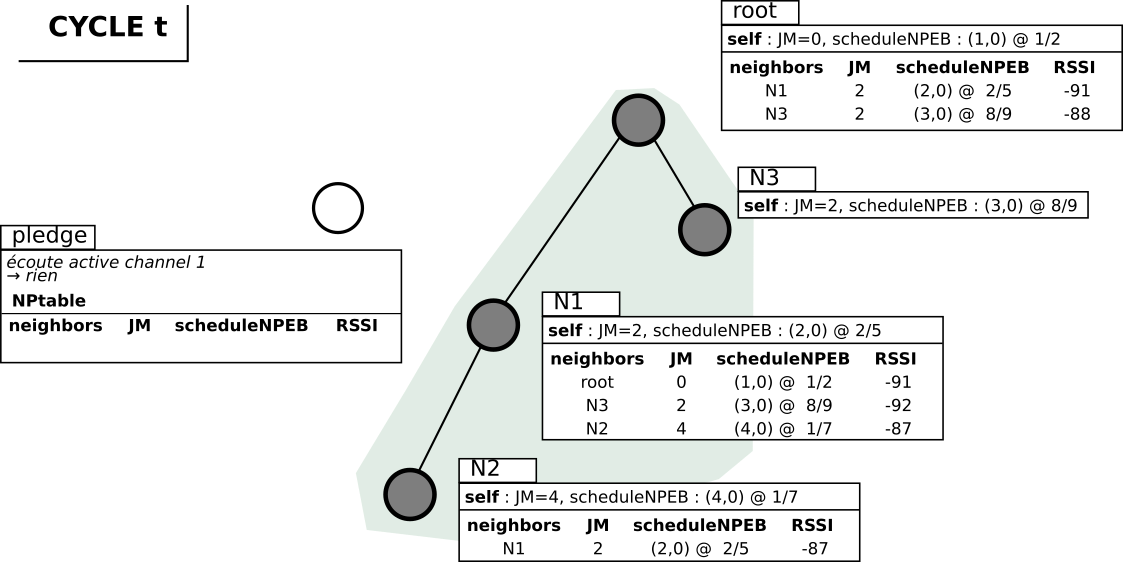
\includegraphics[width=0.85\linewidth]{NPEB_step1}
	\caption{[Cycle t] État initial du réseau où les NPtables des noeuds sont déjà alimentées}
	\label{fig:NPEB_step1}
	\end{figure}
\vspace{0.2cm}

La \wordlink{Figure}{fig:NPEB_step1} illustre l'état initial du réseau considéré au cycle t, c'est-à-dire correspondant à la valeur d'ASN $lenSF * t$ où $lenSF$ est la taille de la slotframe. Les noeuds du réseau ont déjà des informations sur certains de leur voisin, maintenues dans leur NPtable. La notation pour le schedule NPEB correspond à \textit{cell} @ \textit{curr\_cycle}/\textit{nbr\_cycles}. Durant ce cycle t, le pledge écoute activement sur le channel 1 (stratégie arbitraire), mais aucun NPEB n'est émis (\textit{curr\_cycle} n'est à 0 pour aucun noeud).

 \vspace{0.6cm}
	\begin{figure}[!h]
	\centering
	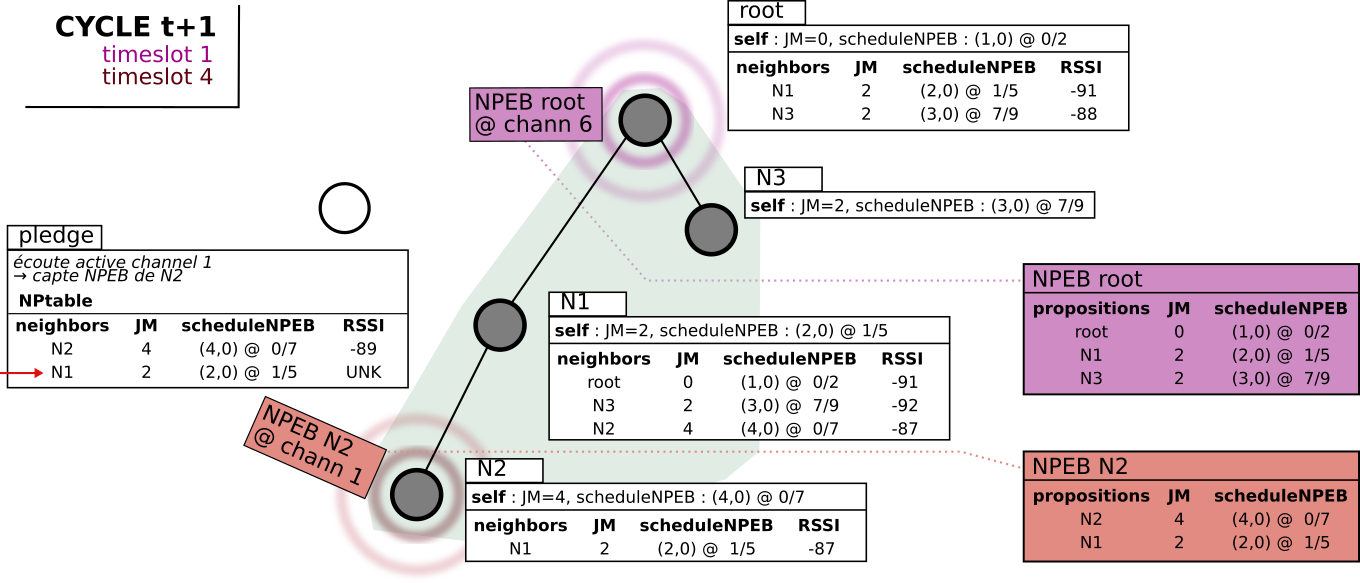
\includegraphics[width=\linewidth]{NPEB_step2}
	\caption{[Cycle t+1] Une itération de slotframe écoulée, deux NPEBs programmés pour ce nouveau cycle}
	\label{fig:NPEB_step2}
	\end{figure}
\vspace{0.2cm}

\newpage

La \wordlink{Figure}{fig:NPEB_step2} représente ce qu'il se passe durant le cycle suivant le cycle t. Les compteurs \textit{curr\_cycle} pour chaque voisin stocké dans les NPtables ont été décrémentés, ainsi que ceux propre à chaque noeud. Les compteurs de la cell (1,0) du noeud \textit{root} et la cell (4,0) du noeud N2 sont tombés à 0, chacun a alors installé la cell correspondante dans sa slotframe. Au timeslot 1, le noeud root émet donc un NPEB à un channel offset de 0, qui correspond au channel 6 pour l'ASN courant (valeur pour l'exemple). Les voisins sélectionnés depuis sa NPtable pour être annoncés le sont par un processus décisionnel décrit dans la \wordlink{Section}{decisional}. Le pledge écoute toujours activement sur le channel 1 et n'entend donc pas cet NPEB. En revanche, le NPEB émis par N2 au timeslot 4 est entendu car le channel résultant est le channel 1 qu'il écoute. Il remplit sa propre NPtable en conséquence et utilise une procédure de décision décrite dans la \wordlink{Section}{decisional} pour décider quelle action opérer. Ici, il s'avère que N1 semble un voisin intéressant et a priori meilleur que N2 en se basant sur la Join Metric. Donc, le noeud va passer en sommeil et se réveiller un cycle plus tard pour entendre le NPEB émis par N1 dans la cell (2,0).

 \vspace{1cm}
	\begin{figure}[!h]
	\centering
	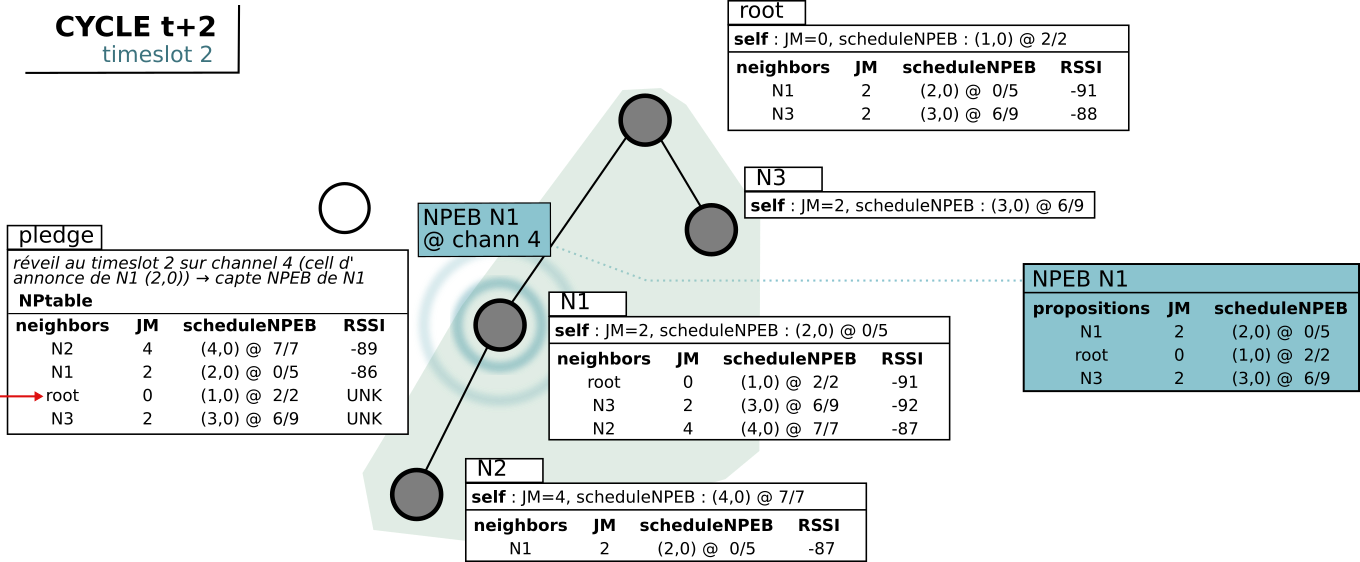
\includegraphics[width=\linewidth]{NPEB_step3}
	\caption{[Cycle t+2] sommeil du pledge jusqu'à la cell d'annonce indiquée par N1}
	\label{fig:NPEB_step3}
	\end{figure}
\vspace{0.4cm}

La \wordlink{Figure}{fig:NPEB_step3} illustre le pledge se réveillant au timeslot 2 du cycle suivant, pour écouter sur ce qu'il calcule comme étant le channel 4. Comme prévu, il entend un NPEB émis par N1 qui est à portée. Ici, la procédure de sélection des voisins à annoncer n'a pas retenu le noeud N2 sur base de sa Join Metric moins bonne que celle des candidats root et N3. Le pledge complète sa NPtable avec l'information sur ces nouvelles propositions de voisin et obtient une indication du RSSI avec le noeud N1 grâce à la frame qu'il vient de capturer. Obtenant les coordonnées d'une cell d'annonce de root, il décide de se rendormir les deux cycles suivants pour l'écouter. Effectivement, si root est à une portée raisonnable, il sera d'office le meilleur voisin (en terme de Join Metric) et lancer le processus de join avec ce dernier sera très avantageux (pas de noeud intermédiaire, accès le plus direct vers le JRC). De plus, une fois le processus de join terminé (devenu joined node) et root sélectionné comme preferred parent dans la topologie, cela permettra d'établir une route la plus courte possible vers le Root du DODAG. Ce sera également avantageux si le joined node vient à servir de noeud intermédiaire, par exemple en servant de Join Proxy quand il commence à émettre des (NP)EBs.

\newpage

 \vspace{0.4cm}
	\begin{figure}[!h]
	\centering
	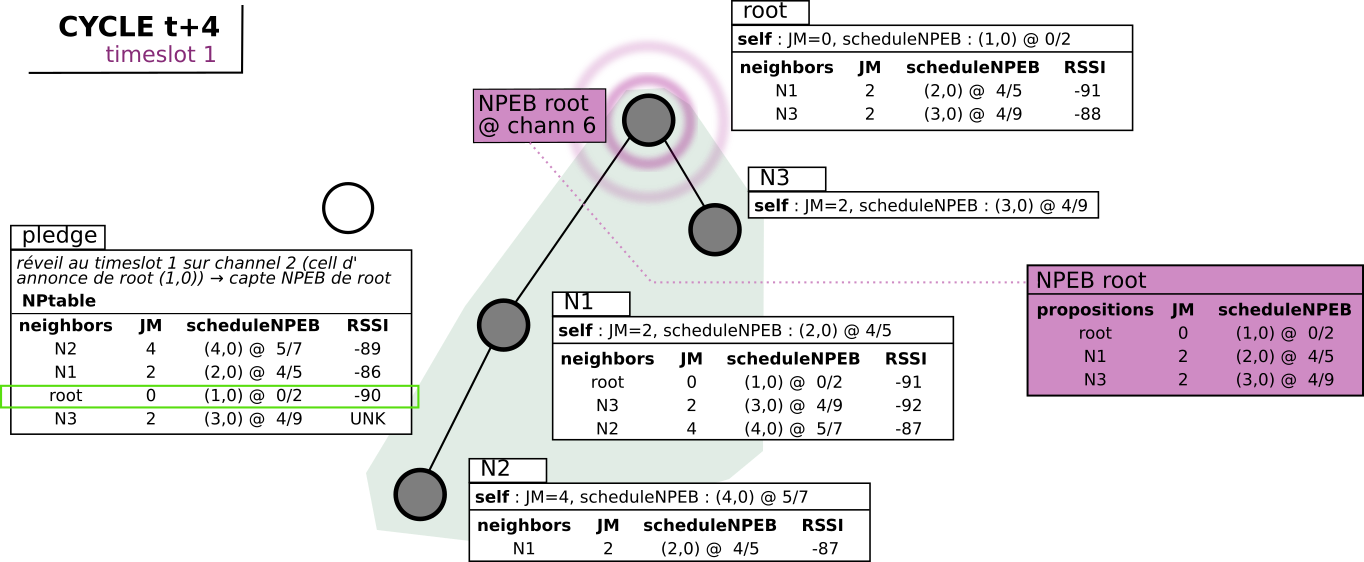
\includegraphics[width=\linewidth]{NPEB_step4}
	\caption{[Cycle t+4] sommeil du pledge jusqu'à la cell d'annonce indiquée par root et lancement de la suite du processus de join avec celui-ci}
	\label{fig:NPEB_step4}
	\end{figure}
\vspace{0.4cm}

La \wordlink{Figure}{fig:NPEB_step4} correspond à la dernière itération, quand le pledge se réveille deux cycles plus tard et capte le NPEB émis par root. Il a la confirmation que root est à portée et ne trouve pas d'autre voisin plus intéressant à écouter dans sa NPtable. Il va donc lancer la suite de la joining phase avec root. Il est synchronisé temporellement avec le réseau et suppose son adresse IPv6 link-local valide, il s'agit donc d'émettre sa Join Request CoJP comme décrit à la \wordlink{Section}{global_CoJP}. Une fois qu'il aura obtenu le matériel de sécurité du réseau (clés 802.15.4 déployées) et un rang dans la topologie RPL, il sera à même d'émettre des NPEBs dans un cell qu'il sélectionne. Ces NPEBs pourront se base sur l'information déjà présente dans la NPtable, et les cells d'annonces également pour éviter les conflits avec des voisins connus.\\

Cet exemple illustre la façon dont la méthode NPEB tente d'atteindre le double objectif établi en début de cette Section. Le fait qu'une fois un premier NPEB entendu, un pledge ne soit plus obligé de continuer une écoute active pour obtenir des informations sur d'autres voisins constitue un gain en énergie pour lui. La rapidité du processus itératif dépend des procédures de décisions décrites dans la \wordlink{Section}{decisional}, mais supprime en partie la composante aléatoire de la recherche active d'EB. La méthode vise également à lancer la suite de la procédure de join avec le meilleur voisin possible, comme illustré ici  où le pledge part d'une capture de NPEB du noeud N2 mais finit par s'adresser au Root du DODAG pour son intégration au réseau.

\subsection{Méthodes de remplissage de la NPtable}
\label{feed_NPtable}

\subsubsection{NPEB-based}

Cette méthode est la mécanique de base sur laquelle se repose le processus itératif d'écoute des NPEBs. Une sélection des voisins à proposer est effectuée (voir \wordlink{Section}{decisional}, idem pour les deux méthodes suivantes de cette section) à chaque envoi de NPEB. En pratique, l'information est encodée dans un Header IE 802.15.4 tel que brièvement décrit dans la \wordlink{Section}{EBs} et standardisé dans \cite{IEEE802.15.4}. Cet IE est rajouté à la fin du Header MAC et est transmis en clair, comme décrit dans la \wordlink{Section}{IEEE802.15.4-sec}.\\

La spécification \cite{rfc8180} stipule qu'un joined node devrait ignorer tout EB reçu mais peut toujours écouter à la recherche d'EBs émis par un autre réseau. Ici, comme les NPEBs émis par un noeud du même réseau peuvent transporter de l'information utile pour mettre à jour la NPtable, ils ne sont pas ignorés mais a priori cette réception est le fruit du hasard. Afin d'adapter dynamiquement la NPtable d'un joined node, les méthodes Data-based et ACK-based présentées dans la suite de cette Section sont utilisées.

\subsubsection{Data-based}

Lors d'un échange de données quelconque, une frame est échangée entre deux voisins. De la même façon que pour les NPEB, des propositions de voisins peuvent être passées à travers un IE 802.15.4. Cependant, on peut envisager ici l'utilisation d'un Payload IE qui serait donc chiffré au niveau lien afin de divulger le moins possible les schedules NPEB des noeuds du réseau, même si cela restera de toute façon le cas avec les NPEBs. Il faut alors tenir compte de l'overhead du chiffrement, et de façon générale veiller à ne pas entrainer de fragmentation si le payload de la frame est conséquent.\\

Les voisins qui échangent des frames augmentées avec des propositions de voisins le font pour mettre à jour leur NPtable et la remplir avec de nouveaux noeuds. Le schéma qui est intuitivement le plus intéressant est du trafic downstream, venant d'un noeud plus haut dans la topologie. Les voisins qu'un tel noeud propose seront meilleurs en terme de Join Metric que pour du trafic upstream, et donc plus avantageux à annoncer dans les NPEBs destinés aux pledge.

\subsubsection{ACK-based}

Le principe est identique aux voisins proposés avec la méthode Data-based, mais en ne considérant que les ACKs 802.15.4 qui supportent également les IEs. Cependant, utiliser des ACK pour communiquer des propositions de voisins est plus avantageux. Premièrement, comme expliqué pour la méthode Data-based, les voisins proposés devraient préférentiellement venir d'un noeud plus haut dans la topologie. Pour les ACKs, c'est donc le cas avec du trafic upstream (l'ACK est renvoyé par le parent). C'est ce type de trafic qui est majoritaire dans l'IIoT \cite{openbenchmark}. Secondement, les ACKs ne transportent pas de payload des couches supérieures et sont donc extensibles avec plus d'information, tout en restant chiffrables \cite{IEEE802.15.4}.

\subsection{Procédures décisionnelles et paramétrage}
\label{decisional}

Cette Section décrit les différentes procédures pour les prises de décisions impliquées dans la méthode NPEB, à différents niveaux. Ces procédures sont adaptables en fonction du comportement escompté, les définitions qui en sont données ici sont basiques et destinées à servir de \textit{baseline} effective dans un contexte général. Si des modifications sont apportées, elles devraient l'être en tenant compte du fait que ces procédures tournent sur des équipements restreints où des calculs complexes devraient être évités.

\subsubsection{Sélection des voisins à annoncer}

Cette procédure intervient lorsqu'un noeud du réseau \textit{node} souhaite proposer des voisins dans sa prochaine frame qui peut être un NPEB, du transport de payload des couches plus hautes ou un ACK (voir \wordlink{Section}{feed_NPtable}). \textit{Node} a alors un certain nombre de voisins dans sa NPtable qu'il peut proposer, quelque soit le statut d'écoute : s'il est \texttt{None} ou mis à \texttt{0}, rien n'a été reçu de ce voisin mais cela n'exclu pas qu'il envoie des NPEBs tel que annoncé selon le schedule NPEB associé. \textit{Node} souhaite sélectionner parmi ces voisins quels sont les plus avantageux à annoncer, du point de vue d'un noeud qui recevrait ces propositions.\\

La \wordlink{Procédure}{proc_announce} est une façon basique de déterminer les \texttt{NBR\_MAX\_NEIGH\_ANNOUNCED} meilleurs voisins à annoncer, basée sur la Join Metric. Elle associe un score à chaque voisin, diminué par la Join Metric qui se situe dans [0, 255] où une faible valeur indique une bonne place dans la topologie RPL (seul le noeud Root du DODAG atteint la valeur 0). Afin de diriger un comportement convergent vers les noeuds plus hauts de la topologie (illustré par l'exemple de la \wordlink{Section}{intuition_NPEB}), le preferred parent de \textit{node} est favorisé et son score est augmenté. De même si le voisin considérer est Root du DODAG.\\

\newpage

Cette procédure est très simple et a du sens, mais elle peut être affinée en tenant compte de, par exemple, les valeurs \textit{curr\_cycle} de chaque voisin. L'intuition est de donner une préférence aux voisins qui vont bientôt émettre un NPEB (valeur de \textit{curr\_cycle} faible, voire 0 si dans le cycle courant). Considérant \textit{max\_cycle} la valeur la plus élevée parmi les \textit{curr\_cycle} des voisins, une façon simple de procéder serait d'insérer après la ligne 4 une augmentation du score en dépendant ($score \leftarrow score +  maxcycle - $\textit{NPtable}$[neighbor][\text{\textit{curr\_cycle}}]$).

\vspace{0.3cm}
\begin{algorithm}[!h]
\caption{selectNeighborsToAnnounce : sélection des meilleurs voisins à annoncer par le noeud \textit{node}}
\begin{algorithmic}[1]
\Require \textit{NPtable} de node, \texttt{NBR\_MAX\_NEIGH\_ANNOUNCED}
\Ensure Une liste de maximum \texttt{NBR\_MAX\_NEIGH\_ANNOUNCED} voisins connus de \textit{node}
\State $scoredNeighbors \leftarrow [\ ]$
\For{\textit{neighbor} $\in$ \textit{NPtable}}
\State $score \leftarrow 255$
\State $score \leftarrow score\ - $ \textit{NPtable}[\textit{neighbor}][\texttt{joinMetric}]
\If{\textit{neighbor} est Root de la topologie \textbf{ou} preferred parent de \textit{node}}
\State $score \leftarrow score * 2$
\EndIf
\State ajouter le couple (\textit{neighbor}, \textit{score}) à \textit{scoredNeighbors}
\EndFor
\State trier \textit{scoredNeighbors} par ordre décroissant sur le \textit{score}
\State\Return les $1^{\text{ère}}$ composantes des \texttt{NBR\_MAX\_NEIGH\_ANNOUNCED} premiers éléments de \textit{scoredNeighbors}
\end{algorithmic}
\label{proc_announce}
\end{algorithm}
\vspace{0.2cm}

La procédure pourrait également tenir compte de la valeur des RSSI des voisins pour lesquels elle est connue. Bien qu'elle n'ait pas de sens du point de vue du noeud qui reçoit les propositions, elle indique quels noeuds sont proches de \textit{node}. Dans le cas d'une annonce NPEB, \textit{node} peut proposer préférentiellement un voisin avec lequel il a un très bon RSSI, vraisembalement proche. Un pledge qui capte le NPEB et considère l'écoute de ce voisin sera surement également capable d'entendre le NPEB dudit voisin, bien que cela ne soit pas garanti pour autant.

\vspace{0.2cm}

\subsubsection{Sélection d'un candidat voisin parmi ceux proposés au pledge}

Comme décrit dans la \wordlink{Section}{intuition_NPEB}, un pledge qui souhaite continuer le processus itératif pour entendre davantage de NPEBs doit sélectionner un voisin suivant à écouter. Ce voison est choisi parmi les propositions apprises jusqu'ici, stockées dans la NPtable du pledge. La sélection n'est pas faite au hasard mais en se basant sur une procédure  définie qui permet de dégager le voisin le plus intéressant pour le pledge selon plusieurs critères.\\

La \wordlink{Procédure}{proc_listen} est une procédure basique pour sélectionner le meilleur voisin à écouter en se basant sur la Join Metric. Elle fonctionne sur le même principe que la \wordlink{Procédure}{proc_announce}. Cependant, dans ce cas-ci, les voisins qui ont déjà été entendus ou pour lesquels l'écoute du NPEB à la cell indiquée a été infructueuse sont écartés. Un seul voisin est retourné par la procédure.\\

Tout comme mentionné pour la \wordlink{Procédure}{proc_announce}, cette procédure pourrait être modifiée pour prendre en compte le cycle courant \textit{curr\_cycle} associé à chaque cell de voisin proposé. Sélectionner un voisin qui programme d'émettre un NPEB dans les cycles à venir, ou même qui a installé une cell pour le faire dans l'itération de slotframe courante (\textit{curr\_cycle} = 0), peut permettre d'accélerer le processus car le pledge dormira moins longtemps. En revanche, l'information du RSSI n'est ici pas exploitable puisqu'on ne s'intéresse qu'au voisins proposés encore non entendus (RSSI = \texttt{None}).

\newpage

\begin{algorithm}[!h]
\caption{selectNeighborToListen : sélection du meilleur voisin à écouter parmi ceux proposés}
\begin{algorithmic}[1]
\Require \textit{NPtable} courante du pledge contenant des propositions de voisins (non vide)
\Ensure Un voisin considéré comme le meilleur à écouter ensuite pour capter son NPEB
\State $scoredNeighbors \leftarrow [\ ]$
\For{\textit{neighbor} $\in$ \textit{NPtable}}
\If{\textit{NPtable}[\textit{neighbor}][\texttt{RSSI}] $\neq $ \texttt{None} }
\State passer le reste de cette itération de boucle
\Else
\State $score \leftarrow 255$
\State $score \leftarrow score\ - $ \textit{NPtable}[\textit{neighbor}][\texttt{joinMetric}]
\If{\textit{neighbor} est Root de la topologie \textbf{ou} preferred parent de \textit{node}}
\State $score \leftarrow score * 2$
\EndIf
\State ajouter le couple (\textit{neighbor}, \textit{score}) à \textit{scoredNeighbors}
\EndIf
\EndFor
\If{\textit{scoredNeighbor} est vide}
\State\Return \texttt{None}
\EndIf
\State trier \textit{scoredNeighbors} par ordre décroissant sur le \textit{score}
\State\Return la $1^{\text{ère}}$ composante du premier élément de \textit{scoredNeighbors}
\end{algorithmic}
\label{proc_listen}
\end{algorithm}


\subsubsection{Processus itératif d'écoute de NPEBs}

La \wordlink{Procédure}{proc_iter} est la formalisation du processus itératif illustré dans la \wordlink{Section}{intuition_NPEB}. Elle est appelée à la réception d'un NPEB par un pledge qui n'a pas encore décidé avec quel voisin il lancera son processus de join complet. Un pledge dans cette situation maintient une référence \textit{bestNP} qui indique quel est selon ses connaissances le meilleur candidat courant. Également, il maintient un timer courant décrémenté au fur et à mesure des périodes actives. Il sert à trancher si le pledge n'a lancé la suite de son processus de join avec aucun voisin après un temps donné (assimilable à \texttt{MAX\_EB\_DELAY} de la spécification \cite{rfc8180}). La situation de départ est que le pledge a sa \textit{NPtable} vide, \textit{bestNP} à \texttt{None} et le timer \textit{remainingListenDelay} initialisé à 180 secondes. Il lance alors un écoute active sur un channel au hasard, jusqu'à ce qu'un NPEB soit capté et la \wordlink{Procédure}{proc_iter} appelée (\textit{remainingListenDelay} s'écoulera à partir de ce moment lors des prochaines phases d'écoute active).\\

Une fois le NPEB reçu, il est parsé premièrement comme un EB standard et deuxièmement la partie Neighbors Propositions est traitée. La fonction feedTable(.) met à jour et rempli la NPtable du pledge avec les informations sur les voisins proposés. De plus, le voisin \textit{neighbor} qui a émis le NPEB est considéré de la même façon (le pledge a en plus une valeur pour le RSSI associé). La fonction isBetterNeighbor(\textit{n1}, \textit{n2}) est appelée sur deux voisins dont un NPEB a été reçu et retourne vrai si \textit{n1} a une meilleure Join Metric et un meilleur RSSI que \textit{n2}.\\

La fonction shouldUndergoSynchroWith(\textit{node}) permet de trancher quand arrêter le processus itératif et est donnée par la \wordlink{Procédure}{proc_stop} (détaillée plus loin). Elle utilise tous les éléments connus du pledge pour décider si un candidat devrait être celui avec lequel lancer la suite du processus de join. Le candidat est ici \textit{bestNP}, le meilleur voisin dont un NPEB a été capté par le pledge jusqu'ici, en prenant en compte le NPEB \textit{NPEB} qui vient d'être reçu. La fonction carryOnJoiningWith(.) correspond au lancement de la suite du processus de join (Join Exchange CoJP) non détaillée ici car indépendante de l'utilisation de la méthode NPEB. À noter que les échanges subséquents auront alors lieu dans la minimal cell tel que décrit par la spécification \cite{rfc8180}, ou gérés par la Scheduling Function (MSF utilise par exemple les autonomous cells, voir \wordlink{Section}{scheduling}).\\

\newpage

\begin{algorithm}[!h]
\caption{receiveNPEB : traitement de l'évènement réception d'un NPEB en écoute active}
\begin{algorithmic}[1]
\Require \textit{NPtable} du pledge, \textit{NPEB}, \textit{bestNP}=\texttt{None}, \textit{remainingListenDelay}=\texttt{180}
\Ensure Le pledge a pris une décision à partir de sa connaissance du réseau
\State feedTable(\textit{NPtable}, \textit{NPEB})
\State \textit{neighbor} $\leftarrow$ \textit{NPEB}[\texttt{self}]
\If{\textit{bestNP} est \texttt{None} \textbf{ou} isBetterNeighbor(\textit{neighbor}, \textit{bestNP})}
\State \textit{bestNP} $\leftarrow$ \textit{neighbor}
\EndIf
\If{shouldUndergoSynchroWith(\textit{NPtable}, \textit{bestNP})}
\State carryOnJoiningWith(\textit{bestNP})
\Else
\State \textit{mostInterestingNP} $\leftarrow$ selectNeighborToListen(\textit{NPtable})
\If{\textit{mostInterestingNP} est \texttt{None}}
\State [lancer écoute active pour \textit{remainingListenDelay} secondes
\State avec fonction de callback carryOnJoiningWith(\textit{bestNP})]
\Else
\State \textit{scheduleIntNeigh} $\leftarrow$ \textit{NPtable}[\textit{mostInterestingNP}][\texttt{scheduleNPEB}]
\State \textit{targetASN} $\leftarrow$ computeNPEBAnnouncementASN(\textit{scheduleIntNeigh})
\State [passer en sommeil jusque réveil à \textit{targetASN} pour écouter NPEB de \textit{mostInterestingNP}
\State suivi d'une écoute active de \textit{remainingListenDelay} secondes si rien reçu
\State avec fonction de callback carryOnJoiningWith(\textit{bestNP})]
\EndIf
\EndIf
\end{algorithmic}
\label{proc_iter}
\end{algorithm}

\vspace{0.2cm}


La fonction selectNeighborToListen(.) est la \wordlink{Procédure}{proc_listen} détaillée précédemment. Si elle ne retourne aucun voisin (ligne 10), alors le pledge retourne en écoute active pour les \textit{remainingListenDelay} secondes restantes et décrémentera de fait ce timer. S'il arrive à expiration, le processus de join sera lancé avec \textit{bestNP}. Si un NPEB est reçu en écoute active durant cet intervalle de temps, la procédure receiveNPEB est à nouveau appelée (nouvelle itération).\\

Si en revanche un voisin intéressant est retourné par selectNeighborToListen(.) (ligne 13), le pledge récupère le schedule NPEB associé à ce voisin depuis la NPtable. Il sait alors dans combien de cycles (\textit{curr\_cycle}) il va installer une cell d'annonce de NPEB. La fonction computeNPEBAnnouncementASN(.) opère des calculs simples pour calculer l'ASN à laquelle cette annonce aura lieu. Il va ensuite passer en sommeil jusqu'à ce moment, où il se réveille pour recevoir le NPEB. S'il est capté, la procédure receiveNPEB est à nouveau appelée pour une nouvelle itération du processus d'écoute. Sinon, le pledge repasse en écoute active comme détaillé précédemment dans le cas \textit{mostInterestingNP} = \texttt{None}.\\


La fonction shouldUndergoSynchroWith(.) est détaillée par la \wordlink{Procédure}{proc_stop}.
Elle permet de décider si un voisin dont un NPEB a été reçu est un voisin qui présente des caractéristiques suffisantes que pour être utilisé dans la suite du processus de join. Elle retourne donc un booléen qui, s'il est \texttt{Vrai}, mettra fin au processus itératif d'écoute de voisin. La décision s'opère sur plusieurs critères, sous forme de seuils paramétrables. Dans un premier lieu, le RSSI doit être suffisamment élevé (ligne 2) que pour avoir des échanges fiables. Pour se faire, une conversion en terme de PDR est faite, basée sur une table établie empiriquement présentée dans \cite{simulating-6TiSCH}. Ensuite, si le noeud est le Root de la topologie (ligne 6), on sait que le PDR est correct par la proposition précédente et donc qu'il faut aller vers ce noeud. Si ce n'est pas le cas, la Join Metric annoncée doit être assez bonne que pour garantir une bonne place dans la topologie (ligne 9). À noter que le seuil \texttt{MAX\_JM\_UNDERGO\_SYNCHRO} à 0 revient à imposer qu'il soit Root et donc validé par la déclaration précédente, le paramétrage doit se faire en fonction de l'Objective Function utilisée par RPL. Finalement, si le voisin a passé les précédentes conditions, et que tous les voisins proposés ont déjà été écoutés (ligne 13), alors il est choisi pour continuer le processus de join. 

\newpage

\begin{algorithm}[!h]
\caption{shouldUndergoSynchroWith : décision d'arrêt pour le processus itératif validant le voisin candidat pour la suite du processus de join}
\begin{algorithmic}[1]
\Require \textit{NPtable} courante du pledge, \textit{neighbor} voisin candidat, \texttt{MIN\_PDR\_UNDERGO\_SYNCHRO}=\texttt{0.6}, \texttt{MAX\_JM\_UNDERGO\_SYNCHRO}=\texttt{0}
\Ensure \texttt{Vrai} ssi le processus itératif doit être stoppé
\State \textit{pdr} $\leftarrow$ rssiToPdr(\textit{NPtable}[\textit{neighbor}][\texttt{RSSI}])
\If{pdr $<$ \texttt{MIN\_PDR\_UNDERGO\_SYNCHRO}}
\State\Return \texttt{Faux}
\EndIf
\State \textit{neighJM} $\leftarrow$ \textit{NPtable}[\textit{neighbor}][\texttt{joinMetric}]
\If{\textit{neighJM} == 0}
\State\Return \texttt{Vrai}
\EndIf
\If{\textit{neighJM} $>$ \texttt{MAX\_JM\_UNDERGO\_SYNCHRO}}
\State\Return \texttt{Faux}
\EndIf
\If{plus de 2 voisins dans \textit{NPtable}}
\If{il ne reste plus de voisin à écouter dans \textit{NPtable} (ont tous RSSI $\neq$ \texttt{None})}
\State\Return \texttt{Vrai}
\EndIf
\EndIf
\State\Return \texttt{Faux}
\end{algorithmic}
\label{proc_stop}
\end{algorithm}
\vspace{0.4cm}

\subsection{Discussion des optimisations possibles}
\label{optis_NPEB}

Cette Section fait l'état de plusieurs optimisations apportables à la méthode NPEB telle que présentée dans les Sections précédentes. L'intuition qui les justifie est donnée pour chacune. Lors des expérimentations, les optimisations considérées dans l'implémentation seront mentionnées avec les résultats.

\subsubsection{Placement des cells d'annonce}

Les noeuds du réseau peuvent a priori choisir n'importe quelle cell arbitrairement, excepté celles du timeslot 0 puisque la minimal cell y est installée. Cependant, il est intéressant de pouvoir les disposer de sorte qu'un pledge puisse enchainer les itérations du processus d'écoute avec le moins de temps mort passé en sommeil entre deux NPEBs. Si la minimal cell est utilisée pour émettre des NPEBs, il est donc avantageux que les timeslots suivants soient considérés en priorité pour y installer des cells d'annonce de NPEB. Ainsi, le pledge recevant un NPEB en tout début d'itération de slotframe se voit proposer des voisins dont les cells d'annonce s'enchainent directement les timeslots suivants.\\

Les noeuds du réseau peuvent tirer parti de leur NPtable pour sélectionner leur(s) cell(s) d'annonce intelligemment. Effectivement, le schedule NPEB associé à chaque voisin renseigne les coordonnées des cells qui sont donc déjà utilisées. Un noeud sélectionne donc le premier timeslot de la slotframe qu'aucun voisin connu n'exploite déjà. Il sélectionne le channel offset de façon aléatoire. La \wordlink{Figure}{fig:NPEB_cells} illustre l'enchainement des cells d'annonce au début de la slotframe. Le fait que certaines cells soient installées par plusieurs noeuds n'est pas génant comme ils ne sont à priori pas voisins l'un pour l'autre (sinon un timeslot différent aurait été choisi).\\

Cependant, un pledge qui rate le début de la slotframe devra attendre sa prochaine itération. Pour éviter cela et avoir une répartition minimum, un noeud qui installe une deuxième cell d'annonce le fait suivant le même processus mais en considérant un timeslot minimum qui est la moitié de la slotframe. S'il vient à installer une troisième cell, il considérera un timeslot minimum au tier de la slotframe, etc.

\newpage

 \vspace{1cm}
	\begin{figure}[!h]
	\centering
	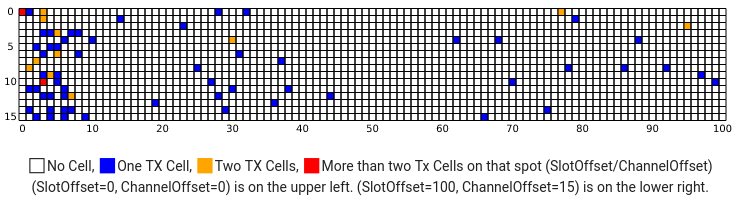
\includegraphics[width=0.95\linewidth]{NPEB_cell}
	\caption{Illustration de la sélection de cell tirée du simulateur 6TiSCH \cite{simulating-6TiSCH} modifié pour supporter la méthode NPEB}
	\label{fig:NPEB_cells}
	\end{figure}

\vspace{0.6cm}

\subsubsection{Nombre de cycles}

Une fois les coordonnées d'une cell d'annonce décidées, un noeud doit évaluer le nombre de cycles \textit{nbr\_cycles} qui séparera chaque annonce. Intuitivement, un noeud qui a une mauvaise place dans la topologie devrait émettre moins de (NP)EBs que ses parents. Une façon de refléter cela dans le nombre de cycles est de le choisir proportionnelement à la valeur de la Join Metric du noeud. Plus la Join Metric est élevée (le neoud a une moins bonne place dans la topologie), plus \textit{nbr\_cycles} le sera également.\\

Une stratégie faisant intervenir le nombre de voisins connus peut également être envisagée, à la manière du broadcast Bayesien \cite{broadcast-strategies}. Ici, il est envisageable d'augmenter \textit{nbr\_cycles} pour espacer les émissions de NPEB au plus le noeud a de voisins connus.
~\\
\subsubsection{Cycles décalés entre voisins}

Le fait que les annonces ne soient pas opérées à chaque itération de slotframe peut éventuellement mener à une situation de ``famine". L'exemple le plus flagrant est si l'on considère deux noeuds voisins dans la topologie qui ont la même Join Metric. Par la Section précédente, ils calculent pour une cell d'annonce un même \textit{nbr\_cycle}. Si \textit{curr\_cycle} est également identique, ils sont alignés et émettent toujours dans des itérations de slotframes simultanées. Un pledge dans le voisinnage peut alors écouter activement des cycles durant sans entendre ni l'un ni l'autre.\\

Une façon simple et non coûteuse de contrer cela est de considérer le \textit{curr\_cycle} connu des voisins quand une nouvelle cell d'annonce est créée. Si possible, le \textit{curr\_cycle} initial sera mis à une valeur non utilisée par les voisins qui annoncent au même \textit{nbr\_cycles}. Éventuellement, les multiples peuvent aussi être pris en compte pour être complet. Il en résulte un décalage de cycles entre les annonces et un étalement sur le temps évitant les temps d'écoute active trop longs pour les pledges.
~\\
\subsubsection{Cell \textit{RxS} après une annonce NPEB}

La méthode NPEB permet à un pledge de trouver efficacement un bon voisin, mais une fois celui-ci choisi il reste au pledge à effectuer la suite de son processus de join (Join Exchange CoJP). Cela se fait indépendamment de la méthode NPEB, en utilisant la minimal cell si la Scheduling Function en activité ne prévoit aucun mécanisme dédié. Ce n'est pas le cas de MSF qui installe des autonomous cells temporaires dédiées au trafic de join (voir \wordlink{Section}{scheduling}), le raisonnement suivant n'est donc pas pertinent si MSF est utilisée. Les performances globales du join sont donc encore impactées par l'usage de celle-ci, tel que décrit dans la \wordlink{Section}{min_cell}.\\

\newpage

Pour éviter la congestion dans la minimal cell, il est envisageables que les noeuds du réseaux installent d'autres cells destinées à la réception de la Join Request CoJP émise par un noeud qui souhaite continuer son processus de join. Une manière d'intégrer cela à la méthode NPEB est de prévoir un nouveau champ \textit{nbr\_rx\_cycles\_after} dans le schedule NPEB de chaque noeud. \textit{nbr\_rx\_cycles\_after} indique le nombre de cycles suivants l'annonce d'un NPEB de la part du noeud où celui-ci installe une cell \textit{RxS}, aux mêmes coordonnées (donc \textit{nbr\_rx\_cycles\_after} $<$ \textit{nbr\_cycles}). Pour un pledge qui vient d'entendre un NPEB et de valider le voisin pour continuer son processus de join, cela lui permet d'envoyer sa Join Request vers le noeud au cycle suivant, évitant de le faire dans la minimal cell. Le noeud se mettra en écoute à ce moment et pourra traiter la Join Request CoJP comme si elle était reçue de façon standard dans la minimal cell. La suite du processus de join se déroule normalement, la Join Response CoJP sera relayée vers le pledge dans la minimal cell.\\

Le principal inconvénient de procéder de la sorte est la perte d'énergie liée à l'installation régulière d'une cell \textit{RxS}, où le noeud peut écouter dans le vent si aucun pledge ne lance son processus de join avec lui. Idéalement, \textit{nbr\_rx\_cycles\_after} est donc mis à 1. Ce qui signifie que le noeud installe la cell \textit{RxS} quand \textit{curr\_cycle} = \textit{nbr\_cycles} mais pas pour les cycles suivants. Cette technique est intuitivement plus avantageuse durant la phase de bootstrapping du réseau où la minimal cell est fortement utilisée, tous les noeuds essayant de rejoindre presque simultanément.

\newpage

\section{Inconvénients de la méthode NPEB}

\subsection{Non conformité avec le standard MSF}

La méthode NPEB ne respecte pas strictement la spécification de MSF \cite{ietf-6tisch-msf-10}. Celle-ci fait l'hytpothèse que la minimal cell est la seule utilisée pour l'émission d'EBs et de DIOs. Les autonomous cells que MSF installe sur base d'un hash de l'EUI-64 des noeuds communiquants tiennent comptent de cette contrainte et ne peuvent être installées au timeslot 0. En revanche, tous les autres timeslots sont valides, ce qui peut donc interférer avec les timeslots choisis pour les cells d'annonce de NPEB.\\

En pratique, cela n'est que modérément génant car les cells d'annonce peuvent être déplacées, l'impact sera alors que la modification du schedule NPEB devra se répandre parmi les voisins qui proposent le noeud en question. Cela peut mener à une situation où un pledge planifie l'écoute d'une annonce NPEB qui n'arrivera jamais car la cell a été déplacée. Pour éviter cette situation, on peut tirer part du fait que les coordonnées des autonomous cells que MSF installe sont fixées et connues à l'avance (dérivées de l'EUI-64 du noeud cible). Les timeslots réservés de la sorte à l'installation d'autonomous cell sont d'avance exclus de ceux considérés pour programmer les cells d'annonce. De plus, les negotiated cells ne sont installées par MSF qu'aux timeslots libres donc non pris par une cell d'annonce NPEB. Ces dernières sont négociées entre voisins, donc les annonces NPEB de chacune des parties sont prises en compte.

\subsection{Overhead des messages et NPtable}

Sont évalués ici l'overhead induit par les propositions de voisin dans des IEs 802.15.4 et le montant d'informations à stocker en mémoire pour maintenir la NPtable. On suppose ici que les noeuds sont identifiés de façon unique par leur adresse MAC.

\subsubsection{Proposition de voisin}
\label{size_prop}

Émettant un NPEB, un noeud renseigne ceux qui le reçoivent sur lui même. Son adresse MAC et sa Join Metric sont des champs de l'EB standard. La réception de la frame en elle-même permet de dériver la valeur de RSSI associable à ce noeud par le receveur. Le seul champ additionnel à propos de lui-même ajouté par le NPEN est le schedule NPEB du noeud. Il contient une ou des cells d'annonces que le noeud souhaite propager dans le réseau. À chaque cell sont associées les valeurs de \textit{curr\_cycle} et \textit{nbr\_cycles}. Pour la négociation de cells, la spécification \cite{rfc8480} encode une cell sur 4 bytes, ce que l'on considére également ici. On peut raisonnablement considérer un maximum de 15 cycles entre deux annonces de NPEB, et donc considérer 1 byte pour l'information relative aux cycles (4 bits pour \textit{curr\_cycle} et \textit{nbr\_cycles}). La valeur \texttt{0x00} est une valeur spéciale utilisée pour renseigner le fait que la cell n'est plus à considérer pour les annonces (le noeud n'émettra plus de NPEB dans celle-ci). Au total, un schedule NPEB renseignant une cell d'annonce est donc encodable sur 5 bytes.\\

Un NPEB contient une liste de propositions de voisins, chacun identifié par son adresse MAC, donc 6 bytes. À chaque voisin est associé la valeur de sa Join Metric (1 byte) et son schedule NPEB (idem que décrit précédemment). Pour faciliter le parsing, il est nécessaire de donner pour chaque scedule NPEB le nombre de cells qu'il renseigne (raisonnablement 4 bits suffisent). De même, le nombre de voisins proposés $n$ doit être indiqué (raisonnablement 4 bits suffisent). Au total, proposer $n$ voisins est encodable sur
 \[ 4+n (6*8 + 1*8 + 4 + \text{nbrcells}_{i}*5*8) 
 %= 4+n(48+8+4+\text{nbrcells}_{i}*40) 
 = 4 + n(60+\text{nbrcells}_{i}*40)\ \text{bits} \]
 
À titre d'exemple, un NPEB proposant deux voisins qui renseignent chacun une cell introduit un overhead brut (sans compter les champs descriptifs de l'IE 802.15.4 \textit{Type-Length}) de $[5*8] + [4+2*(60+40)] = 244$ bits $\approx 30$ bytes. La taille d'un EB n'est pas fixée et peut varier, par exemple si l'extension d'EB \cite{ietf-6tisch-enrollment-enhanced-beacon-14} est utilisée. \cite{ATP} indique que la taille mininmum d'un EB est de 40 bytes. La taille maximum d'une frame 802.15.4 étant de 127 bytes (voir \wordlink{Section}{802.15.4PHY}), cela laisse une marge raisonnablement suffisante pour annoncer plus de deux voisins.

\newpage

\subsubsection{Stockage de la NPtable}

Les noeuds du réseau ont un espace mémoire limité, aussi la NPtable doit être maintenue de sorte à ne pas stocker d'information futile. Une estimation de la place que les données brutes occupent peut être obtenue de la même façon qu'à la \wordlink{Section}{size_prop}. La structure utilisée pour les stocker est dépendante de l'implémentation et n'est pas détaillée ici.\\

La maintenance de la NPtable doit se faire de façon intelligente en considérant les informations qu'elle fournit. Un procédé de nettoyage de la NPtable doit être lancé régulièrement pour décider de quelles sont les propositions de voisins qui doivent être préservées. Intuitivement, les voisins dont l'écoute à la cell annoncée à échoué (\textit{RSSI} = \texttt{0}) sont ceux à écarter en priorité. La \wordlink{Procédure}{proc_announce} (selectNeighborsToAnnounce()) peut être réutilisée pour décider de quels sont les meilleurs voisins à maintenir dans la NPtable. Les détails de la procédure ne sont pas présentés ici.


\section{Implémentation de la méthode NPEB}
\label{implem_NPEB}

Comme détaillé dans le Chapitre suivant à la \wordlink{Section}{choice_sim}, la méthode NPEB est implémentée comme une extension du simulateur 6TiSCH écrit par le WG 6TiSCH \cite{simulating-6TiSCH}. Le code existant est modifié afin de pouvoir supporter la méthode NPEB, et des structures telles que la NPtable sont ajoutées aux informations qu'un noeud maintient. Le simulateur modifié est accessible sur GitHub\footnote{\url{https://github.com/RemDec/6tisch-simulator-NPEB}}. Comme l'intégration est faite dans le code même, les changements sont limités à la partie de l'implémentation représentant la couche 2 d'un noeud (802.15.4 en mode TSCH), qui est intégralement reprise dans le fichier \texttt{SimEngine/Mote/tsch.py}. D'autres changements mineurs sont effectués pour journaliser les nouveaux évènements et définir le nouveau type d'EB.\\

L'implémentation faite implémente les procédures décrites dans la \wordlink{Section}{decisional}. Les méthodes de remplissage de la NPtable considérées sont les méthodes NPEB-based et ACK-based présentées dans la \wordlink{Section}{feed_NPtable}. La méthode Data-based est écartée car les expérimentations se concentrent sur la joining phase ou le trafic applicatif n'est pas important. Finalement, les optimisations proposées dans la \wordlink{Section}{optis_NPEB} sont toutes implémentées à l'exception de la cell RxS après une annonce NPEB, celle-ci n'étant pas pertinente quand la Scheduling Function est MSF.


\chapter{Évaluation de la joining phase sécurisée et de la méthode NPEB en simulateur}
\label{chap_exp}
\newpage

\section{Choix du simulateur}
\label{choice_sim}

Une comparaison des simulateurs et émulateurs supportant la pile réseau 6TiSCH est établie dans \cite{simulating-6TiSCH}. Le simulateur 6TiSCH, présenté dans ce même article, a été sélectionné pour mener la phase expérimentale de ce travail. Il a été écrit par les membres du WG 6TiSCH et cible spécifiquement la pile étudiée, ce qui simplifie d'une part son utilisation et d'autre part son extensibilité. Il s'agit d'un simulateur dit \textit{discrete event-driven}, c'est-à-dire qu'il n'émule pas la pile 6TiSCH au niveau binaire, mais plutôt du point de vue comportemental. Cependant, il parvient à simuler de façon fidèle le déploiment de la pile en situation réelle \cite{simulating-6TiSCH}. En addition au simulateur 6TiSCH, un framework de traitement de ses sorties développé au Service Réseaux et Télécommunications est utilisé. Il permet de manipuler les lancements du simulateur et les données journalisées, par le biais d'une surcouche écrite en Python.

\section{Méthodologie}

\subsection{Déroulement des expérimentations}

Les expérimentations sont divisées en deux parties. La première s'intéresse à la joining phase telle que décrite dans les spécifications 6TiSCH, que le simulateur implémente conformément. Cependant, comme le simulateur se restreint au niveau comportemental, l'échange CoJP est bien simulé mais les traitements cryptographiques liés à OSCORE (dérivation de contextes, chiffrement/déchiffrement) ne sont pas pris en compte. Ces expérimentations visent à évaluer quel est l'impact de l'échange CoJP sur la joining phase. Des métriques pertinentes sont choisies pour illustrer au mieux les différences en considérant ou non l'usage de la sécurité dans la joining phase (demandant le Join Exchange CoJP). La seconde partie évalue la méthode NPEB présentée dans le \wordlink{Chapitre}{chap_NPEB}, la comparant à un déploiement standard. D'autres métriques pertinentes sont sélectionnées pour observer les effets de la méthode NPEB sur la formation du réseau. Chaque résultat obtenu est discuté et justifié.\\

Les variations étudiées ici se concentrent sur des modifications du déroulement de la joining phase, et non des caractéristiques du réseau en lui-même (nombre de noeuds, etc.). Le simulateur 6TiSCH permet de configurer ces caractéristiques, imposant des contraintes sur le réseau simulé. Pour toutes les expériences, une disposition des noeuds aléatoire est utilisée, mais elle est soumise à des contraintes que le simulateur respecte au mieux \cite{simulating-6TiSCH}. Ainsi, on impose que chaque noeud doit avoir au minimum 3 voisins avec lesquels il a un lien caractérisable par un PDR minimum de 0.5. Pour se placer dans la situation d'un déploiement basique conforme au standard, la Scheduling Function considérée est MSF pour toutes les expérimentations. Afin de rester dans des temps de calcul d'ordre raisonnable pour la reproductibilité de celles-ci, le nombre de runs (simulation sur une nouvelle instance de réseau) est limité à 10.\\

La \wordlink{Section}{impact_secjoin} illustre l'impact de l'usage de la sécurité sur la formation du réseau. Un réseau de 10 noeuds est considéré pour l'évaluer. Comme ces expériences se concentrent uniquement sur la joining phase, aucune application n'est simulée sur chacun des noeuds, le trafic est donc relatif aux couches plus basses exclusivement. Les expériences sont orchestrées en utilisant le framework développé au Service Réseaux et Télécommunications, qui fonctionne par dessus une version du simulateur 6TiSCH modifiée mais permettant un comportement conforme au standard.\\

La \wordlink{Section}{eval_NPEB} étudie les performances de la méthode NPEB en comparaison avec un déploiement standard. Afin d'établir la viabilité de la méthode, le réseau considéré contient 30 noeuds, tel que cela peut être le cas dans des déploiements réels \cite{openbenchmark}. Une application qui envoie des paquets périodiquement toutes les 60 secondes est instanciée sur chaque noeud, ce trafic interférant avec la méthode NPEB. Le simulateur 6TiSCH de base est modifié tel que décrit dans la \wordlink{Section}{implem_NPEB}, et de nouvelles méthodes d'écriture et de traitement des logs sont ajoutées pour illustrer les métriques pertinentes. Le framework n'est donc pas utilisé ici. Afin de supporter les mêmes métriques et les nouvelles procédures de traitement des sorties, le simulateur 6TiSCH de base est augmenté \footnote{\url{https://github.com/RemDec/6tisch-simulator-joinmetrics.git}}.

\newpage

\subsection{Paramètrage des procédures de join}
\label{exp_custom}

\subsubsection{Déploiement standard (EBs)}

\subsubsection{Déploiement avec la méthode NPEB}

\newpage

\section{Impact de la sécurité sur la formation du réseau}
\label{impact_secjoin}

\subsection{Sélection des métriques}

\subsubsection{Temps de convergence}

Le \textit{temps de convergence} désigne la durée nécessaire pour que chaque noeud déployé  rejoigne le réseau. Dans le cas où la sécurité est désactivée, il s'agit donc de sélectionner un voisin dont un EB est reçu et s'y synchroniser. Si elle est activée, après cette étape, il doit encore compléter le Join Exchange CoJP pour récupérer le matériel de sécurité du réseau. Il est donc attendu que dans le cas où la sécurité est activée, on observe un temps de convergence plus long dû au Join Exchange CoJP qui se fait avec le noeud Root du réseau.

\subsubsection{Temps de join individuel}

Le temps de join pour chaque noeud a la même sémantique que pour le temps de convergence (en fonction de la présence ou non de sécurité). Il est mesuré individuellement pour chaque noeud du réseau. Cela permet d'illustrer le fait que la sécurité ralentit le join pour chaque noeud considéré, et pas uniquement au niveau global.

\subsection{Présentation et discussion des résultats}

\subsubsection{Temps de convergence}

Les temps de convergencs récupérés pour les 10 runs et avec/sans sécurité du join sont représentés par la \wordlink{Figure}{fig:convergence}. La simulation a été paramétrée de sorte qu'elle ne se termine pas avant la convergence, et ce pour toutes les runs.

	\begin{figure}[!h]
	\centering
	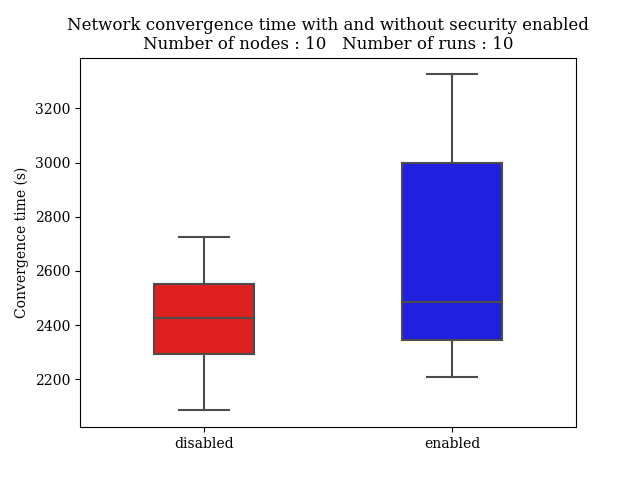
\includegraphics[width=0.7\linewidth]{results/secjoin/boxesTimeConvergence10.png}
	\caption{Temps de convergence d'un réseau de 10 noeuds, mesuré sur 10 runs}
	\label{fig:convergence}
	\end{figure}

\vspace{0.1cm}
On observe le phénomène attendu : l'usage de la sécurité dans le join rallonge le temps de convergence du réseau. En moyenne sur les 10 runs (donnée par la ligne pointillée), sans la sécurité le réseau converge en 40 minutes, tandis ce qu'avec il converge en 45 minutes. Cependant, l'écart-type est deux fois plus élevé avec la sécurité : 414 secondes contre 202 secondes sans. Cela est explicable par le fait que le Join Exchange CoJP doit traverser l'entièreté du réseau et opérer plusieurs sauts où des retransmissions peuvent être nécessaires.

\newpage


\subsubsection{Temps de join individuel}

La \wordlink{Figure}{fig:join_times} illustre l'impact de l'usage de la sécurité au niveau individuel, pour chaque noeud du réseau excepté le noeud Root qui a déjà rejoint à l'initialisation de la simulation. Ces mesures sont prises sur les mêmes runs que pour le temps de convergence. 

 \vspace{0.2cm}
	\begin{figure}[!h]
	\centering
	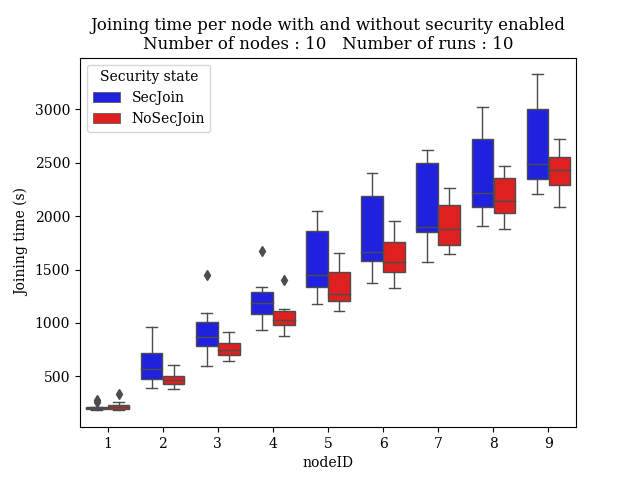
\includegraphics[width=0.7\linewidth]{results/secjoin/boxesJoiningTimePerNode10.png}
	\caption{Temps de join pour 10 noeuds composant le réseau, mesuré sur 10 runs}
	\label{fig:join_times}
	\end{figure}

Le même phénomène qu'au niveau global est observable : l'usage de la sécurité ralentit le join, et ce pour chaque noeud du réseau.

\subsection{Discussion globale des résultats} 

De par les résultats obtenus, la sécurisation du réseau a un impact non négligeable sur le temps nécessaire à sa formation. Pour rappel, le simulateur ne prend pas en compte les opérations cryptographiques en tant que tels : seul le Join Exchange est simulé. Dans un déploiement réel, l'usage de la sécurité implique des coûts additionnels. D'une part, le chiffrement utilisé dans 802.15.4 pour sécuriser les frames a un coût non négligeable qui peut aller jusqu'à nécéssiter une augmentation de la durée des timeslots. Cela dépend du chiffrement utilisé, de l'utilisation d'hardware dédié, etc. : un travail qui cible cette problématique a été réalisé par Sciancalepore \textit{et al.} \cite{link-layer-sec-impact}. D'autre part, la sécurité au niveau applicatif (OSCORE) n'est pas prise en compte et impacte potentiellement la joining phase. Très peu de données peuvent être trouvées à ce propos : Durand \textit{et al.} \cite{OSCOREtimes} mesurent le temps nécessaire pour le chiffrement/déchiffrement d'un paquet de 6 bytes à $\approx 1.3$ secondes sur un microcontrôleur SAML11 ARM Cortex-M23. Gündoğan \textit{et al.} \cite{OSCOREvsNDN} établissent une comparaison entre OSCORE et d'autres solutions de chiffrement applicatif mais ne rentrent pas en détail dans les performances d'OSCORE.

\newpage

\section{Amélioration des performances par la méthode NPEB}
\label{eval_NPEB}


\subsection{Sélection des métriques}

\subsubsection{Temps cumulé lors des étapes du join}
\label{metric_times}

Afin de détailler les variations induites par la méthode NPEB, la joining phase est découpée en trois étapes successives :
\begin{enumerate}
\item la synchronisation : désigne le moment où un pledge décide de lancer la suite du processus de join avec un de ses voisins connus (appris au travers de (NP)EBs)
\item l'intégration sécurisée au réseau : désigne le moment où un pledge reçoit sa Join Response et qu'il installe les informations qu'elle contient
\item l'intégration à la topologie : désigne le moment où un pledge reçoit le premier DIO qu'il peut déchiffrer après avoir rejoint le réseau, lui permettant de se greffer à la topologie RPL
\end{enumerate}
\vspace{0.2cm}
À chaque run, pour chaque noeud, l'instant à laquelle ce dernier passe une étape est journalisé. Ces mesures sont prises en temps absolu depuis l'initialisation du réseau (ASN 0) et sont converties en secondes.

\subsubsection{Charge consommée cumulée lors des étapes du join}
\label{metric_charges}

Comme discuté dans la \wordlink{Section}{intuition_NPEB}, la méthode NPEB permet intuitivement à un pledge de sauvegarder de l'énergie. Cependant, cela ne devrait pas se faire au prix d'une consommation d'énergie accrue par les noeuds du réseau qui annoncent les NPEBs. Pour illustrer cela, la charge consommée par chaque noeud est récupérée à chaque étape du join process, telles que décrites précédemment dans la \wordlink{Section}{metric_times}. De plus, une étape supplémentaire est considérée une fois le join process terminé. On considère une attente de \texttt{DELAY\_LOG\_AFTER\_EB} secondes après que le désormais joined node soit autorisé à émettre des (NP)EBs (dans l'implémentation, après avoir envoyé un DAO de sorte que le Root aprenne la route vers le noeud). Après ce délai, une mesure de la charge est prise : elle a pour objectif de donner une indication de la consommation énergétique que l'annonce de (NP)EBs entraîne. À noter que l'application génère du trafic pendant cette durée, mais elle le fait de la même façon dans le cas des EBs et NPEBs. les étapes auxquelles sont prises les mesures de charge sont donc les suivantes :

\begin{enumerate}
\item la synchronisation
\item l'intégration sécurisée au réseau
\item l'intégration à la topologie 
\item \texttt{DELAY\_LOG\_AFTER\_EB} secondes après ``l'autorisation" d'émission de (NP)EBs
\end{enumerate}
\vspace{0.2cm}
À chaque run, pour chaque noeud, la charge consommée jusqu'à ce que ce dernier passe une étape est journalisée. Ces mesures sont prises en coulombs, de manière absolue depuis l'initialisation du réseau (ASN 0).

\subsubsection{Première position dans la topologie}
\label{metric_hops}

La \wordlink{Section}{intuition_NPEB} mettait en avant un autre bénéfice intuitivement attribuable à la méthode NPEB : la position avantageuse dans la topologie du voisin sélectionné. Afin de l'illustrer, le nombre de sauts effectués par le premier paquet applicatif de chaque noeud (destiné au Root) est journalisé. Les simulations sont configurées de sorte que chaque noeud ait le temps d'émettre un tel paquet après avoir rejoint le réseau. À noter que le voisin avec lequel un pledge décide de lancer son processus de join n'est pas systématiquement celui qui sera son preferred parent au moment de transmettre son premier paquet applicatif. Cette métrique est donc légèrement biaisée.

\subsubsection{Latence sur le trafic}

La latence correspond à l'interval de temps nécessaire à un paquet pour arriver à sa destination. Intuitivement, si le nombre de sauts est globalement réduit avec la méthode NPEB, la latence devrait être impactée positivement. Cette métrique permet également de vérifier que la méthode NPEB n'impacte pas négativement les échanges applicatifs. Il s'agit d'une métrique disponible de base dans le simulateur 6TiSCH.

\subsubsection{Longévité du réseau}
\label{metric_lifetime}

L'estimation de la longévité d'un noeud est une autre métrique proposée par le simulateur 6TiSCH. La consommation moyenne de courant du noeud \textit{avg\_current\_uA} est d'abord estimée en se basant sur la charge totale consommée à la fin de la simulation et du temps écoulé depuis la synchronisation du noeud. En faisant l'hypothèse que le noeud est alimenté par une pile AA (2821.5 \textit{mAh}), la métrique estime le nombre d'années d'activité du noeud de la sorte :
\[
\text{\textit{lifetime\_AA\_years}} = \frac{2821.5 \times 1000}{\text{\textit{avg\_current\_uA}}}
\frac{1}{24 \times 365}
\]

Cette estimation permet de vérifier que la méthode NPEB n'impacte pas négativement la consommation énergétique des noeuds.

\subsection{Présentation et discussion des résultats}

\subsubsection{Temps cumulé lors des étapes du join}
\label{results_times}

Les \wordlink{Figures}{fig:EBtimes} et \ref{fig:NPEBtimes} illustrent respectivement les temps cumulés pour le déploiement standard et la méthode NPEB. Il s'agit, pour chaque étape, des temps récupérés sur toutes les runs pour tous les noeuds du réseau (aucune distinction n'est faite entre eux). Le trait pointillé représente la moyenne de chaque distribution. La ligne verticale bleue représente le temps moyen de convergence du réseau sur toutes les runs. La \wordlink{Table}{table_times} détaille les distributions des temps pour chaque étape numériquement, pour le cas standard et avec la méthode NPEB.


\begin{figure}[!ht]
	\begin{minipage}{0.49\textwidth}
		\centering
		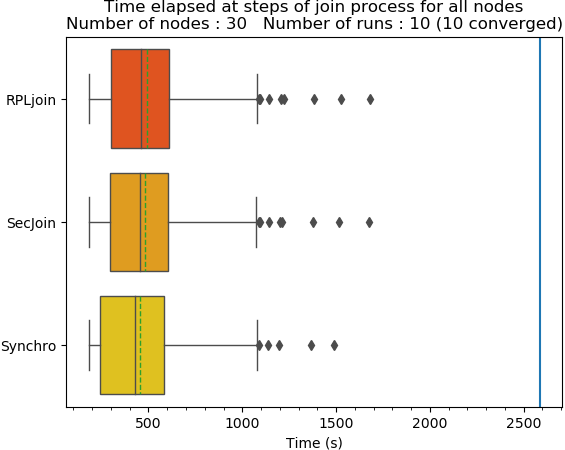
\includegraphics[width=\textwidth]{results/EB/phase_times}
		\caption{EBs - temps cumulé par\\ \noindent étapes du join}
		\label{fig:EBtimes}
	\end{minipage}\hfill
	\begin{minipage}{0.5\textwidth}
		\centering
		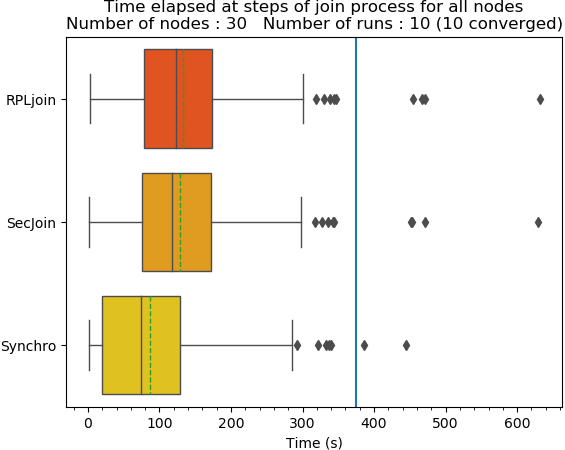
\includegraphics[width=\textwidth]{results/NPEB/phase_times}
		\caption{NPEBs - temps cumulé par\\ étapes du join}
		\label{fig:NPEBtimes}
	\end{minipage}	
\end{figure}

À première vue, la méthode NPEB a un impact non négligables sur la rapidité avec laquelle les noeuds complètent leur processus de join. Les noeuds ont pour la très grande majorité terminé leur join après 8 minutes avec la méthode NPEB, tandis ce qu'à peine environ la moitié l'ont réalisé dans un déploiement standard. Cependant, on observe qu'en moyenne le temps de convergence n'est que légèrement amélioré avec la méthode NPEB (ligne bleue). Cependant, seulement 10 runs sont considérées ici. Le fait que les temps de convergence soient si éloignés est justifiable : l'intégralité des noeuds doivent avoir rejoint. Si un seul noeud très mal disposé est mis en difficulté pour rejoindre le réseau, il impacte directement le temps de convergence. Quand il n'y a pas de tel noeud, la convergence est beaucoup plus rapide : dans ces 10 runs, le minimum pour le déploiement standard est de 26 minutes (1565 secondes) et de 16 minutes (949 secondes) pour la méthode NPEB.

\newpage

\begin{table}[h]
\centering
\begin{tabular}{|l|c|c|c|c|c|c|c|}
	\hline
    \textbf{\textbf{Étape}} & moyenne & écart-type & minimum & Q1 & Q2 & Q3 & maximum\\
    \hline
    \multicolumn{8}{|l|}{\textit{Déploiement standard (EBs)}}\\  
    \hline
    Synchronisation & 543.5 & 227.7 & 181.0 & 244.0 & 428.0 & 580.0 & 1489.7 \\
    \hline
    Join sécurisé & 482.9 & 243.6 & 181.8 & 292.1 & 452.9 & 605.9 & 1677.3 \\
    \hline
    Join topologie RPL & 490.2 & 243.7 & 183.8 & 298.2 & 460.3 & 610.3 & 1680.4 \\
    \hline
    \multicolumn{8}{|l|}{\textit{Déploiement avec la méthode NPEB}}\\    
    \hline
    Synchronisation & 86.9 & 79.1 & 1.0 & 19.7 & 73.7 & 128.0 & 444.4 \\
    \hline
    Join sécurisé & 128.9 & 87.1 & 2.0 & 76.0 & 118.0 & 172.1 & 629.2 \\
    \hline
    Join topologie RPL & 132.6 & 86.6 & 3.0 & 79.0 & 123.5 & 173.2 & 631.2 \\
    \hline
\end{tabular}
\caption{Statistiques des temps mesurés aux différentes étapes du join avec et sans la méthode NPEB (\textit{s})}
\label{table_times}
\end{table}

La \wordlink{Table}{table_times} décrit plus précisément les performances de la méthode NPEB par rapport au déploiement standard. On observe que 75\% des noeuds ont déjà achevé leur join complet (en 173 secondes) quand, pour le déploiement standard, aucun noeud n'a encore lancé sa synchronisation avec un voisin (on observe le délai \texttt{MAX\_EB\_DELAY} de 180 secondes présenté dans la \wordlink{Section}{prob_joining_phase}).



\subsubsection{Charge consommée cumulée lors des étapes du join}
\label{results_charges}

Les \wordlink{Figures}{fig:EBcharges} et \ref{fig:NPEBcharges} représentent la charge totale consommée par tous les noeuds aux différentes étapes considérées, toutes runs confondues. Le délai laissé passé après l'autorisation d'émettre des (NP)EBs (décrit à la \wordlink{Section}{metric_charges}) est de 200 secondes, ce qui correspond à à peu près 200 cycles de slotframe. Les \wordlink{Figures}{fig:EBchargesjoined} et \ref{fig:NPEBchargesjoined} détaillent les distributions de la charge consommée jusqu'à l'accomplissement du join sécurisé, respectivement pour le déploiement standard et la méthode NPEB. La \wordlink{Table}{table_charges} donne les valeurs numériques pour chaque étape considérée.

\vspace{0.2cm}

\begin{figure}[!ht]
	\begin{minipage}{0.49\textwidth}
		\centering
		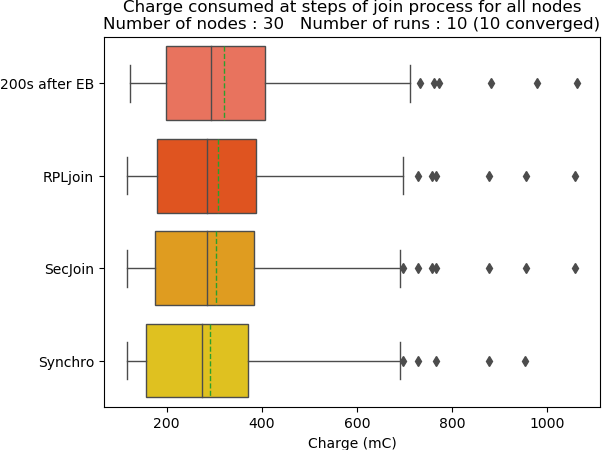
\includegraphics[width=\textwidth]{results/EB/phase_charges}
		\caption{EBs - charges cumulées par étapes du join et par la suite}
		\label{fig:EBcharges}
	\end{minipage}\hfill
	\begin{minipage}{0.5\textwidth}
		\centering
		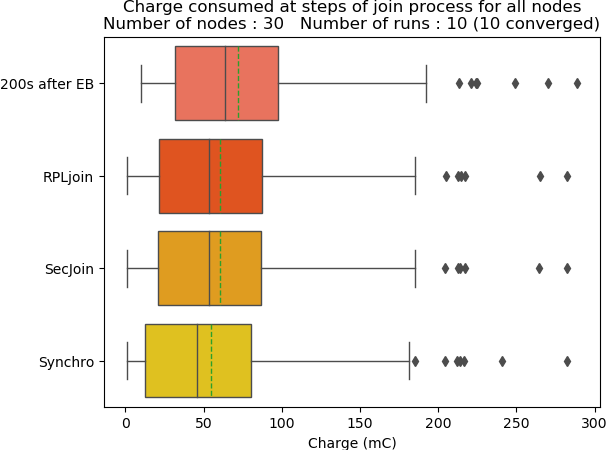
\includegraphics[width=\textwidth]{results/NPEB/phase_charges}
		\caption{NPEBs - charges cumulées par étapes du join et par la suite}
		\label{fig:NPEBcharges}
	\end{minipage}	
\end{figure}

\vspace{0.2cm}


Les \wordlink{Figures}{fig:EBcharges} et \ref{fig:NPEBcharges} mettent en avant un gain de performances pour la méthode NPEB. Pour compléter leur join, 75 \% des noeuds ont consommé une charge inférieur à $100 mC$ en utilisant la méthode NPEB, ce qui n'est le cas que de moins de 25\% des noeuds en déploiement standard. La consommation induite par l'émission de NPEB est relativement minime (détaillée plus loin). La \wordlink{Figure}{fig:NPEBchargesjoined} donne la distribution détaillée jusqu'à l'étape de fin du join sécurisé, qui est bien plus avantageuse que ce qui est obtenu avec le déploiement standard (\wordlink{Figure}{fig:EBchargesjoined}).

\newpage

\begin{figure}[!ht]
	\begin{minipage}{0.49\textwidth}
		\centering
		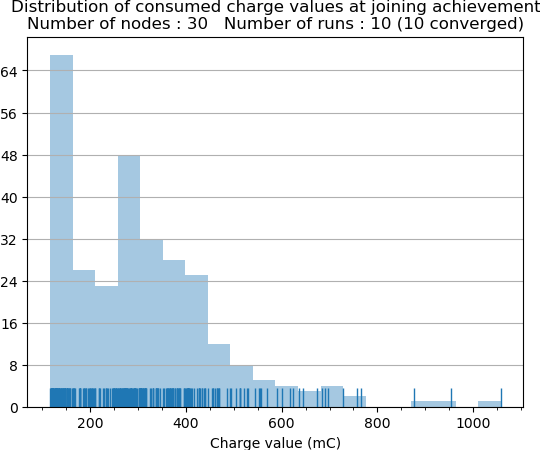
\includegraphics[width=\textwidth]{results/EB/chargejoined.hist}
		\caption{EBs - distribution des charges consommées à la fin du Join Exchange CoJP}
		\label{fig:EBchargesjoined}
	\end{minipage}\hfill
	\begin{minipage}{0.5\textwidth}
		\centering
		\includegraphics[width=\textwidth]{results/NPEB/chargejoined.hist}
		\caption{NPEBs - distribution des charges consommées à la fin du Join Exchange CoJP}
		\label{fig:NPEBchargesjoined}
	\end{minipage}	
\end{figure}

La \wordlink{Table}{table_charges} permet d'avancer qu'en moyenne, un pledge consomme de l'ordre de 5 fois moins d'énergie pour compléter son join en utilisant la méthode NPEB. En moyenne, on observe également que l'énergie consommée 200 secondes après le début d'émission de (NP)EBs est du même ordre entre le déploiement standard et la méthode NPEB. L'impact énergétique induit par l'écoute active est clairement visible en se focalisant sur les valeurs du premier quartile. La méthode NPEB, qui permet de se passer en grande partie de ces phases d'écoute, permet à 25\% des noeuds le rejoindre le réseau en consommant moins de $13 mC$, ce qui représente un facteur supérieur à 10 par rapport au déploiement standard.

\begin{table}[h]
\centering
\begin{tabular}{|l|c|c|c|c|c|c|c|}
	\hline
    \textbf{\textbf{Étape}} & moyenne & écart-type & minimum & Q1 & Q2 & Q3 & maximum\\
    \hline
    \multicolumn{8}{|l|}{\textit{Déploiement standard (EBs)}}\\  
    \hline
    Synchronisation & 290.4 & 145.8 & 115.8 & 156.2 & 274.2 & 371.9 & 953.6\\
    \hline
    Join sécurisé & 304.1 & 155.2 & 115.9 & 176.1 & 285.0 & 383.2 & 1058.1 \\
    \hline
    Join topologie RPL & 307.2 & 155.3 & 116.1 & 179.3 & 285.8 & 386.9 & 1058.3 \\
    \hline
    200s après autorisation EB & 320.2 & 158.0 & 122.9 & 198.3 & 293.1 & 406.0 & 1063.1 \\
    \hline
    \multicolumn{8}{|l|}{\textit{Déploiement avec la méthode NPEB}}\\    
    \hline
    Synchronisation & 54.5 & 49.9 & 0.6 & 12.64 & 45.8 & 80.1 & 282.1 \\
    \hline
    Join sécurisé & 60.2 & 49.8 & 0.7 & 20.9 & 53.2 & 86.9 & 282.3 \\
    \hline
    Join topologie RPL & 60.6 & 49.6 & 0.8 & 21.2 & 53.6 & 87.0 & 282.4 \\
    \hline
    200s après autorisation EB & 71.7 & 50.5 & 9.6 & 31.5 & 63.9 & 97.84 & 289.0 \\
    \hline
\end{tabular}
\caption{Statistiques des charges mesurées pour les étapes considérées avec et sans la méthode NPEB (\textit{mC})}
\label{table_charges}
\end{table}

\subsubsection{Première position dans la topologie}
\label{results_hops}

Les \wordlink{Figures}{fig:EBfirsthop} et \ref{fig:NPEBfirsthop} donnent, respectivement pour le déploiement standard et la méthode NPEB, les distributions du nombre de sauts effectués par le premier envoyé par chaque noeud, toutes runs confondues. Il s'agit donc de la première position effective dans la topologie au niveau applicatif pour chaque noeud, qui peut être amené à sélectionner un autre preferred parent par la suite (non repris ici).

\newpage

\begin{figure}[!ht]
	\begin{minipage}{0.49\textwidth}
		\centering
		\includegraphics[width=\textwidth]{results/EB/firsthop.hist}
		\caption{EBs - distribution du nombre sauts effectués par le 1$^{er}$ paquet des joined nodes}
		\label{fig:EBfirsthop}
	\end{minipage}\hfill
	\begin{minipage}{0.5\textwidth}
		\centering
		\includegraphics[width=\textwidth]{results/NPEB/firsthop.hist}
		\caption{NPEBs - distribution du nombre sauts effectués par le 1$^{er}$ paquet des joined nodes}
		\label{fig:NPEBfirsthop}
	\end{minipage}	
\end{figure}

\vspace{0.2cm}

Les deux distributions sont relativement similaires. La méthode NPEB ne semble par apporté les améliorations attendues, qui se seraient manifesté par une distribution plus lourde pour les petits nombres de sauts. 

\subsubsection{Latence sur le trafic}
\label{results_latence}

Les \wordlink{Figures}{fig:EBlatence} et \ref{fig:NPEBlatence} décrivent les latences moyennes calculées pour chaque noeud, toutes runs confondues. Il s'agit de la latence sur les paquets applicatifs, donc dans ce cas uniquement de trafic upstream dirigé vers le Root (de par la configuration de l'application). Un noeud commence à générer des paquets applicatifs une fois la topologie rejointe et son premier DAO envoyé, le trafic est donc suffisamment conséquent pour être représentatif : les runs tournent pendant 55 minutes et la majorité (75\%) des noeuds ont rejoint après 10 minutes (voir \wordlink{Section}{result_times}).

\begin{figure}[!ht]
	\begin{minipage}{0.49\textwidth}
		\centering
		\includegraphics[width=\textwidth]{results/EB/latency_avg_s}
		\caption{EBs - latences moyennes}
		\label{fig:EBlatence}
	\end{minipage}\hfill
	\begin{minipage}{0.5\textwidth}
		\centering
		\includegraphics[width=\textwidth]{results/NPEB/latency_avg_s}
		\caption{NPEBs - latences moyennes}
		\label{fig:NPEBlatence}
	\end{minipage}	
\end{figure}

Les données obtenues sont similaires pour le déploiement standard et la méthode NPEB. On en déduit que la méthode NPEB n'impacte pas significativement la latence liée aux paquets applicatifs.

\newpage

\subsubsection{Longévité du réseau}
\label{results_lifetime}

Les \wordlink{Figures}{fig:EBlatence} et \ref{fig:NPEBlatence} donnent,  respectivement pour le déploiement standard et la méthode NPEB, les CDFs relatives aux durées de vie estimées pour chaque noeud, toutes runs confondues. La durée de vie est exprimée en années et est estimée selon la procédure décrite dans la \wordlink{Section}{metric_lifetime}.

\vspace{0.2cm}

\begin{figure}[!ht]
	\begin{minipage}{0.49\textwidth}
		\centering
		\includegraphics[width=\textwidth]{results/EB/lifetime_AA_years.cdf}
		\caption{EBs - CDF des durées de vie estimées pour les noeuds du réseau}
		\label{fig:EBlifetime}
	\end{minipage}\hfill
	\begin{minipage}{0.5\textwidth}
		\centering
		\includegraphics[width=\textwidth]{results/NPEB/lifetime_AA_years.cdf}
		\caption{NPEBs - CDF des durées de vie estimées pour les noeuds du réseau}
		\label{fig:NPEBlifetime}
	\end{minipage}	
\end{figure}

\vspace{0.2cm}

Selon cette méthode d'estimation, un noeud alimenté par une pile AA dans un déploiement standard aura une durée de vie de 5 ans maximum (\wordlink{Figure}{fig:EBlifetime}). Considérant l'usage de la méthode NPEB, cette durée de vie est atteinte par plus de 60\% des noeuds (\wordlink{Figure}{fig:NPEBlifetime}). Ces estimations sont cohérentes avec les résultats des mesures sur les charges consommées présentés par la \wordlink{Section}{results_charges}. On peut en conclure que l'usage de la méthode NPEB permet de rallonger la durée de vie du réseau, sous réserve qu'il s'agit d'estimations sur une période de 55 minutes d'activité. Dans un déploiement réel, une fois le réseau ayant convergé, il est attendu qu'il vive plusieurs années durant lesquelles il n'y a pas de nouveau noeud introduit. Les (NP)EBs ont donc une utilité plus relative à la re-synchronisation. Dans cette optique, les fréquences d'émission de NPEB devraient diminuer une fois la réseau ayant convergé, ceux-ci étant  moins pertinents pour un réseau qui a déjà convergé.

\newpage

\subsection{Discussion globale des résultats} 

La méthode NPEB a été élaborée avec un objectif double qui était le suivant :
\begin{itemize}[label=$\bullet$]
\item accélerer et optimiser en terme d'énergie (du point de vue du pledge) le processus de join
\item permettre au pledge de sélectionner le meilleur voisin possible avec lequel initier le processus de join
\end{itemize}

\vspace{0.3cm}

Selon les résultats présentés dans les \wordlink{Sections}{results_times} et \ref{results_charges}, le premier sous-objectif est atteint. En revanche, la \wordlink{Section}{results_hops} indique que le second objectif n'est pas atteint. Cependant, comme mentionné par la \wordlink{Section}{metric_hops} qui présente la métrique, son interprétation est légèrement biaisée si on la prend pour quantifier le fait que le meilleur voisin soit choisi pour le processus de join spécifiquement. Dans les faits, la finalité reste qu'il est souhaitable que les paquets effectuent le moins de sauts possibles, se baser sur ce trafic pour quantifier l'effet de la méthode NPEB fait donc sens. La \wordlink{Section}{results_latence} établit que la méthode NPEB ne génère pas de latence supplémentaire significative dans le réseau. Finalement, la \wordlink{Section}{results_lifetime} donne une estimation de la viabilité de la méthode NPEB sur des plus longues périodes que celles considérées pour les simulations. Les résultats sont positifs en considérant qu'une estimation sur des durées de 55 minutes est représentative.\\

Dans l'ensemble, selon les métriques considérées, la méthode NPEB a montré des gains de performances ou au pire ne provoque aucune perte. Cependant, ces résultats restent intrinsèquement liés à deux choses : la configuration du réseau et les paramètres de la méthode NPEB fixés pour toutes les expérimentations.\\

La configuration du réseau comprend notamment la disposition de la topologie et la densité du réseau en terme de noeuds. Pour les expérimentations décrites dans ce chapitre, la disposition des noeuds était aléatoire, sous des contraintes sur les voisins de chaque noeud imposées au simulateur. En considérant une topologie dite linéaire (les noeuds forment une chaîne depuis le Root), la méthode NPEB a intuitivement moins d'utilité : chaque noeud a peu de voisins et ceux-ci sont vraisembablement trop éloignés pour un pledge (de par la disposition particulière ``en ligne"). La densité du réseau, qui est de fait liée à la disposition de la topologie, a également un impact sur le comportement de la méthode NPEB. Un réseau plus dense augmente le nombre de voisins de chaque noeud. Un noeud émettant des NPEBs pourra alors faire une discrimination pertinente et proposer les meilleurs voisins parmi tous ceux connus. Un pledge sera à même de sélectionner efficacement un bon voisin parmi l'ensemble fourni à sa disposition, ce qu'avec un déploiement standard il ne ferait pas (arrêt de l'écoute active après \texttt{NUM\_NEIGHBORS\_TO\_WAIT}=2 voisins entendus).\\

La méthode NPEB possède de nombreux paramètres et processus décisionnels qui impactent directement son comportement, fixés pour les expérimentations tel que décrit dans la \wordlink{Section}{exp_custom}. Il n'a pas été établi quelles seraient les valeurs optimales de ces paramètres, celles-ci variant vraisembablement en fonction de la configuration du réseau. Les processus décisionnels décrits dans la \wordlink{Section}{decisional} se veulent aussi basiques que possibles afin de servir de base comparative. Les résultats de la méthode NPEB sont donc grandement dépendants de ces éléments configurables.\\

D'autres métriques pourraient être considérer pour quantifier le gain de performances de la méthode NPEB. Par exemple, le duty cycle d'un pledge avant qu'il ne synchronise avec un voisin sélectionné pourrait être comparé avec un déploiement standard. À noter que la \wordlink{Section}{results_charges} permet d'observer directement le résultat qu'aurait un duty cycle peu élevé, entraînant une diminution de la charge consommée.\\

En conclusion, la méthode NPEB apporte de bons résultats par rapport au déploiement standard, en utilisant une configuration basique de la méthode dans un réseau où chaque noeud possède au moins 3 voisins dont les liens sont caractérisés par un PDR supérieur à 50\%. Les expérimentations compilent les résultats obtenus sur 10 runs indépendantes, validant que les gains de performances observés ne sont pas les fruits du hasard.

\chapter*{Conclusion et recommandations}



\bibliographystyle{plain}
\bibliography{biblio}

\end{document}